\documentclass[a4paper,aps,secnumarabic,balancelastpage,amsmath,amssymb,nofootinbib,floatfix]{report}

\usepackage[utf8]{inputenc}
\usepackage{gensymb}
\usepackage{SIunits}
\usepackage{physics}
\usepackage{gensymb}
\usepackage[italian]{babel}
\usepackage{graphicx} 
\usepackage{geometry}
\usepackage{hyperref}
\usepackage{makeidx}
\usepackage{bm}
\usepackage{fullpage}
\usepackage{subfigure}
\usepackage{graphicx}
\usepackage{subcaption}
\usepackage[export]{adjustbox}
\usepackage{wrapfig}
\usepackage{amsmath}
\usepackage{listings}
\hypersetup{
    colorlinks=true,
    linkcolor=blue,
    filecolor=magenta,      
    urlcolor=cyan,
}
\urlstyle{same}



\makeindex
\selectlanguage{italian}

\begin{document}
\title{\textbf{Process mining}}
\author{\textbf{Daniele Gelmini}}
\date{}
\maketitle
\tableofcontents


    A \textit{probabilistic model} is a mathematical framework used to describe the outcomes of random phenomena. In such models, the outcome of an experiment is uncertain, and we cannot predict it deterministically. To build a probabilistic model, we need three fundamental components: 
    \begin{itemize}
        \item The \textit{sample space} $\Omega$: the set of all possible outcomes.
        \item A \textit{sigma field} $\mathcal{A}$: the collection of events (subsets of $\Omega$) on which we can define probabilities.
        \item A \textit{probability function} $P$: a function that assigns a probability to each event in $\mathcal{A}$.
    \end{itemize}
    
    \section{Sample Space}
    The first step in building a probabilistic model is to define the set of all possible outcomes of an experiment. This set is called the \textit{sample space}, denoted by $\Omega$. Each element in $\Omega$ represents a possible outcome of the random experiment.
    \newline
    For example:
    \begin{itemize}
        \item In the case of a coin flip, $\Omega = \{H, T\}$, where $H$ represents heads and $T$ represents tails.
        \item In the case of rolling a standard six-sided die, $\Omega = \{1, 2, 3, 4, 5, 6\}$.
    \end{itemize}
    
    \section{Events}
    An event is any subset of the sample space $\Omega$. For example, if we consider the experiment of rolling a die, an event could be getting an even number, which can be described as $A = \{2, 4, 6\}$.\newline
    Events are central to probabilistic models because they allow us to describe the occurrence of specific outcomes. For example, the event $A$ occurs if the outcome of the experiment is in the set $\{2, 4, 6\}$. There is no order inside a set, i.e. {1,2} = {2,1}. \newline
    If $\Omega$ is finite, the set of the events will be $2^{\Omega} = P(\Omega) = \text{\{set of all the subset of $\Omega$}\}$. \newline
    If $\Omega$=\{H,T\}, then 
    \begin{equation}
        2^{\Omega} = \{\emptyset,\{H\},\{T\},\{H,T\}\}.
    \end{equation}
    Therefore $\Omega$ is in $\Omega$.\newline
    Any subset can be constructed by eliminating any element of $\Omega$, therefore the number of possible subset is $|2^{\Omega}| = 2^{|\Omega|}$. The operator $|\cdot|$ represents its cardinality. 
    
    \paragraph{Operations on Events}
    We can perform various operations on events:
    \begin{itemize}
        \item \textbf{Union}: The event $A \cup B$ occurs if either event $A$ or event $B$ occurs.
        \item \textbf{Intersection}: The event $A \cap B$ occurs if both events $A$ and $B$ occur.
        \item \textbf{Complement}: The event $A^c$ occurs if event $A$ does not occur.
        \item \textbf{Subtraction}: The event $A \ B$ occurs if A occurs but $A \cap B$ doesn't.
    \end{itemize}
    For example, if $A = \{2, 4, 6\}$ and $B = \{1, 2\}$ in the case of rolling a die:
    \begin{itemize}
        \item $A \cup B = \{1, 2, 4, 6\}$ represents rolling an even number or rolling a number less than or equal to 2.
        \item $A \cap B = \{2\}$ represents rolling a number that is both even and less than or equal to 2.
        \item $A^c = \{1, 3, 5\}$ represents rolling an odd number.
    \end{itemize}

    \section{Sigma Field}
    The \textit{sigma field} (or \textit{sigma algebra}) is a crucial concept in probability theory. It represents the collection of events (subsets of the sample space) for which we can assign probabilities. \newline
    Given a sample space $\Omega$, with a set of events $2^\Omega$, any $\mathcal{A}$ that is a subset of $2^\Omega$ (i.e., $\mathcal{A} \subseteq 2^\Omega$) is called a $\sigma$-field. We cannot define a probability space by taking any possible family of subsets, but we must ensure that certain properties are satisfied. \newline
    A sigma field $\mathcal{A}$ must satisfy the following properties:
    \begin{enumerate}
        \item \textbf{Non-emptiness}: The entire sample space $\Omega$ must belong to the sigma field, i.e., $\Omega \in \mathcal{A}$.
        \item \textbf{Closed under complements}: If an event $A \in \mathcal{A}$, then its complement $A^c = \Omega \setminus A$ must also belong to $\mathcal{A}$.
        \item \textbf{Closed under countable unions}: If $A_1, A_2, \dots, A_n$ are events in $\mathcal{A}$, then their union $\bigcup_{n=1}^{\infty} A_n$ must also belong to $\mathcal{A}$.
    \end{enumerate}

    
    \paragraph{Example 1: Tossing a Coin}
    Consider a simple experiment of tossing a coin. The sample space is $\Omega = \{H, T\}$, where $H$ represents heads and $T$ represents tails. The sigma field $\mathcal{A}$ for this experiment can be defined as the collection of all subsets of $\Omega$, i.e.,
    \[
    \mathcal{A} = \{ \emptyset, \{H\}, \{T\}, \Omega \}.
    \]
    This is the \textit{power set} of $\Omega$, which contains all possible events, including the empty set (no outcome), individual outcomes (heads or tails), and the entire sample space. \newline
    Or if $\mathcal{A}$ = \{$\emptyset$, $\Omega$\} any of his subset are a $\sigma-field$ since all of the properties are respected. There are no other possibilities.
    
    \paragraph{Example 2: Rolling a Die}
    For a die roll, the sample space is $\Omega = \{1, 2, 3, 4, 5, 6\}$. The sigma field $\mathcal{A}$ would include all possible subsets of $\Omega$, such as:
    \[
    \mathcal{A} = \{ \emptyset, \{1\}, \{2\}, \dots, \{6\}, \{1, 2\}, \{1, 3\}, \dots, \Omega \}.
    \]
    In this case, the sigma field contains $2^6 = 64$ elements, since the total number of subsets of a set with $n$ elements is $2^n$.
    
    \paragraph{Example 3: Sigma Fields for Infinite Sample Spaces}
    In more complex cases, particularly when dealing with infinite sample spaces, we do not include every subset of $\Omega$ in the sigma field. Instead, we define a sigma field $\mathcal{A}$ that includes a limited number of subsets that satisfy the properties listed above. This ensures that we can still define probabilities on these subsets.
    
    \section{Constructing a Probability Measure}
    Once we have the sample space $\Omega$ and the sigma field $\mathcal{A}$, we define a \textit{probability measure} $P$ on the events in $\mathcal{A}$:
    \begin{equation}
        P: \mathcal{A} \rightarrow [0,1]
    \end{equation}
    The probability measure must satisfy the following conditions:
    \begin{enumerate}
        \item \textbf{Non-negativity}: For any event $A \in \mathcal{A}$, $P(A) \geq 0$.
        \item \textbf{Normalization}: The probability of the entire sample space is 1, i.e., $P(\Omega) = 1$.
        \item \textbf{Countable additivity}: For any sequence of disjoint events $A_1, A_2, \dots \in \mathcal{A}$, i.e. $A_n \in \mathcal{A}$ $\forall n$, $A_n \cap A_m = \emptyset$,$\forall n \neq m$, the probability of their union is the sum of their probabilities:
        \[
        P\left( \bigcup_{n=1}^{\infty} A_n \right) = \sum_{n=1}^{\infty} P(A_n).
        \]
    \end{enumerate}
    The triple ($\Omega$,$\mathcal{A}$, P) will be called \textit{probability space}.
    
    \paragraph{Example: Coin Flip}
    Consider the experiment of flipping a coin. The sample space is $\Omega = \{H, T\}$, $\mathcal{A} = \{ \emptyset, \{H\}, \{T\}, \Omega \}$.
    We define the probability function $P$ as follows:
    \[
    P(H) = p \quad \text{and} \quad P(T) = 1 - p
    \]
    where $0 \leq p \leq 1$. Here, $p$ represents the probability of obtaining heads, and $1 - p$ represents the probability of obtaining tails. P($\Omega$) = 1 and P($\emptyset$) = 0. The latter comes from the property
    \[
    P(A^c) = 1 - P(A)
    \]
    and the fact that $\emptyset = \Omega^c$.
\chapter{What's a process}
    \section{What is a Process?}
    
    A process is a sequence of steps designed to achieve a specific goal, such as approving a loan, obtaining a degree, or booking a flight. Processes are typically standardized, meaning that all executions of the process follow similar patterns. However, processes are flexible and may include certain activities or tasks that can be:
    \begin{itemize}
        \item \textbf{Skipped:} Some steps may not be necessary every time.
        \item \textbf{Repeated:} Certain actions may occur more than once.
        \item \textbf{Optional:} Some activities might not always be performed.
        \item \textbf{Mutually Exclusive:} Only one of a set of tasks may be performed, not both.
        \item \textbf{Executed in Parallel:} Multiple tasks can be carried out simultaneously (e.g., while pre-assessing documents, additional documents might be requested).
    \end{itemize}
    
    Processes are often analyzed through the use of \textbf{event logs}, which capture data on how a process is executed. Each row in an event log table represents an individual event, and events are grouped by \textbf{case IDs} or \textbf{customer IDs}, which identify specific instances of the process. A key characteristic of event logs is that they are ordered by time, with each event associated with a \textbf{time-stamp} to indicate when the action took place. 
    
    The time aspect in Process Mining is crucial, as opposed to Data Mining where time is often treated as a secondary factor. Time can reveal significant insights into how a process evolves, and detecting changes over time is essential for understanding the performance and efficiency of processes. In addition to the time-stamp, each event is linked to an \textbf{activity}, which describes the action that occurred during the event. Other data such as resources or costs can also be recorded but are not always necessary.
    
    \section{The Discovery of Process Models}
    
    One of the primary tasks in Process Mining is to discover a process model from event logs. A \textbf{process model} is a formal representation of the process flow, often visualized as a directed graph. The goal is to translate raw event data into a meaningful model that reflects how the process operates in practice.
    
    A basic algorithm used in the discovery of process models is the \textbf{Dependency Graph}, which is used to visualize the relations between different activities in a process. In a dependency graph:
    \begin{itemize}
        \item We have a starting point and an endpoint for the process.
        \item Each box represents an activity, and arrows between the boxes indicate that one activity is followed by another.
        \item The number of times a particular path is taken can be annotated next to the arrows.
    \end{itemize}
    
    This graphical representation is based on the \textbf{directly-follow relation}, denoted as $x > y$. This means that in at least one case, activity $x$ is immediately followed by activity $y$. These relationships can be documented in tables or through notation using parentheses and exponents to indicate how frequently paths are taken. For example, the exponent indicates how many instances followed that particular path.
    
    \begin{figure}[htbp]
        \centering
        % Prima immagine
        \begin{subfigure}{\textwidth}
            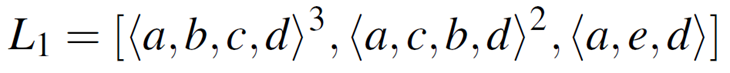
\includegraphics[scale=0.8]{capitolo 2/formula1.png}
        \end{subfigure}
        % Seconda immagine
        \begin{subfigure}{\textwidth}
            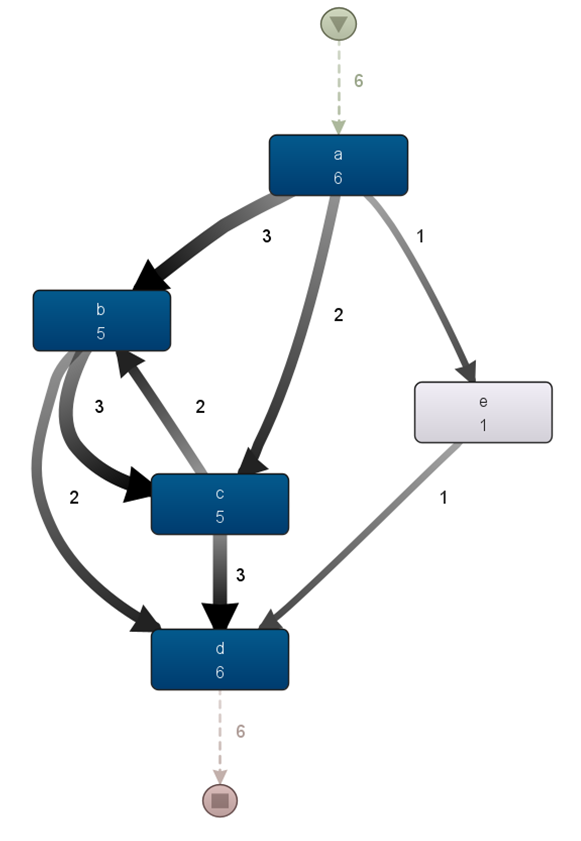
\includegraphics[scale=0.8]{capitolo 2/grafico1.png}
        \end{subfigure}
        % Terza immagine
        \begin{subfigure}{\textwidth}
            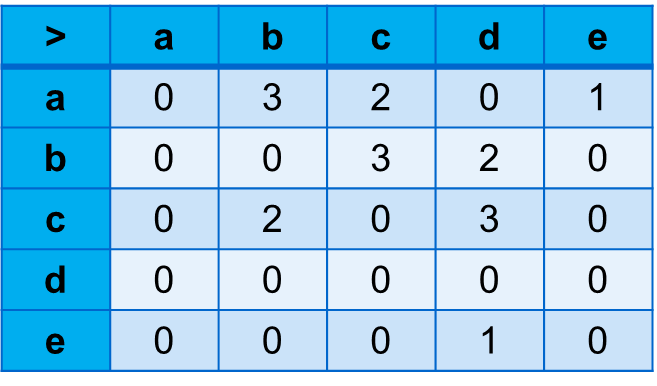
\includegraphics[scale=0.8]{capitolo 2/tabella1.png}
        \end{subfigure}
    \end{figure}
    
    \section{Handling Complexity in Discovery Algorithms}
    
    While the Dependency Graph is a useful way to visualize process flows, it can become unintuitive when certain activities can occur in any order. This is where advanced modeling techniques, such as \textbf{Petri Nets}, come into play. Petri Nets provide a more flexible framework for representing processes where activities may be performed in parallel or in various sequences.
    
    Moreover, processes often include rare or exceptional paths, known as \textbf{infrequent paths}, which may distort the overall representation of the process. These outliers can be filtered out to focus on the \textbf{main stream of behavior}, which represents the most common sequences of activities. By concentrating on the main flow, we gain a clearer picture of the general behavior of the process, while still being able to acknowledge deviations when necessary.

\section{Conditional Probability}
    Given a probability space $(\Omega, \mathcal{A}, {P})$ and two events $A$ and $B$ such that ${P}(B) > 0$ and A,B $\in \mathcal{A}$, the conditional probability of $A$ given $B$ is defined as:
    \[
    {P}(A | B) = \frac{{P}(A \cap B)}{{P}(B)}.
    \]
    This represents the probability of event $A$ occurring under the assumption that event $B$ has already occurred. \newline
    The formula ${P}(A | B)$ quantifies the likelihood of $A$ occurring given that we know $B$ has occurred. If $B$ happens, the sample space effectively shrinks to $B$, and we are interested in the probability that $A$ occurs within this smaller space.
    
    \paragraph{Example 1: Rolling Two Dice}
    Consider two fair dice. Let $A$ be the event that the first die shows a value less than or equal to 2, and let $B$ be the event that the sum of the two dice is 4. We compute ${P}(A | B)$.\newline
    The sample space $\Omega$ consists of all possible pairs $(i,j)$ where $i,j \in \{1, 2, 3, 4, 5, 6\}$, giving us $|\Omega| = 36$. The event $B$, the sum of two dice being 4, consists of the outcomes: 
    \[
    B = \{(1,3), (2,2), (3,1)\},
    \]
    so ${P}(B) = \frac{3}{36} = \frac{1}{12}$.
    The event $A$ consists of the outcomes:
    \[
    A = \{(1,j) | j = 1,2,3,4,5,6\} \cup \{(2,j) | j = 1,2,3,4,5,6\},
    \]
    so ${P}(A) = \frac{12}{36} = \frac{1}{3}$.\newline
    Now, we compute the intersection $A \cap B = \{(1,3), (2,2)\}$, giving ${P}(A \cap B) = \frac{2}{36} = \frac{1}{18}$. Hence, the conditional probability is:
    \[
    {P}(A | B) = \frac{\frac{1}{18}}{\frac{1}{12}} = \frac{2}{3}.
    \]
    This shows that knowing the sum is 4 increases the likelihood of the first die showing a number less than or equal to 2.
    
    \paragraph{Example: Conditional Probability with Balls in a Box}
    We have a box containing 2 white balls and 3 black balls. We withdraw two balls without replacement. Define the following events:
    \begin{itemize}
        \item $B_1$: The first ball is black.
        \item $B_2$: The second ball is black.
    \end{itemize}
    We aim to compute the probability of both $B_1$ and $B_2$ occurring, i.e., $P(B_1 \cap B_2)$. Using the definition of conditional probability, we know:
    \[
    P(B_1 \cap B_2) = P(B_1) \cdot P(B_2 \mid B_1)
    \]
    Computing the Probabilities:
    \begin{itemize}
        \item The probability of drawing a black ball first is:
        \[
        P(B_1) = \frac{3}{5}
        \]
        \item Given that the first ball is black, there are now 2 black balls and 2 white balls left. Thus, the probability of drawing a second black ball is:
        \[
        P(B_2 \mid B_1) = \frac{2}{4} = \frac{1}{2}
        \]
        \item Therefore, the probability of both events occurring is:
        \[
        P(B_1 \cap B_2) = \frac{3}{5} \cdot \frac{1}{2} = \frac{3}{10}
        \]
    \end{itemize}
    Generalizing to $n$ Events: suppose we want to generalize the concept to $n$ events, say $A_1, A_2, \dots, A_n$. The probability of the intersection of these events can be written as:
    \[
    P(A_1 \cap A_2 \cap \dots \cap A_n) = P(A_1) \cdot P(A_2 \mid A_1) \cdot P(A_3 \mid A_1 \cap A_2) \cdot \dots \cdot P(A_n \mid A_1 \cap A_2 \cap \dots \cap A_{n-1})
    \]
    This formula is particularly useful when dealing with sequential events, where each event may depend on the outcomes of the preceding ones. \newline
    We use the law of total probability to express $P(B_2)$:
    \[
    P(B_2) = P(B_1\cap B_2) + P(B_1^c \cap B_2) = P(B_2 \mid B_1) \cdot P(B_1) + P(B_2 \mid B_1^c) \cdot P(B_1^c)
    \]
    Where:
    \begin{itemize}
        \item $P(B_1) = \frac{3}{5}$
        \item $P(B_2 \mid B_1) = \frac{1}{2}$
        \item $P(B_1^c) = \frac{2}{5}$
        \item $P(B_2 \mid B_1^c) = \frac{3}{4}$
    \end{itemize}
    Thus:
    \[
    P(B_2) = \left(\frac{3}{5} \cdot \frac{1}{2}\right) + \left(\frac{2}{5} \cdot \frac{3}{4}\right) = \frac{3}{10} + \frac{6}{20} = \frac{6}{10} = \frac{3}{5}
    \]
    For the case of three elements, we can extend the formula using the law of total probability. The idea is to split the event space in such a way that event \( B_3 \) is expressed in terms of \( B_1 \) and \( B_2 \), as follows:
    \[
    P(B_3) = P((B_1 \cap B_2 \cap B_3)) + P((B_1 \cap B_2^c \cap B_3)) + P((B_1^c \cap B_2 \cap B_3)) + P((B_1^c \cap B_2^c \cap B_3))
    \]
    Now, we can express each term using conditional probabilities. \newline
    The general formula becomes:
    \[
    P(B_3) = P(B_3 \mid B_1 \cap B_2) \cdot P(B_1 \cap B_2) + P(B_3 \mid B_1 \cap B_2^c) \cdot P(B_1 \cap B_2^c)
    \]
    \[
    + P(B_3 \mid B_1^c \cap B_2) \cdot P(B_1^c \cap B_2) + P(B_3 \mid B_1^c \cap B_2^c) \cdot P(B_1^c \cap B_2^c)
    \]
    We can compute each partial probability using the law of total probability, as done in the case of two elements.\newline
    In a more compact form, the formula can be written as:
    \[
    P(B_3) = P(B_3 \mid B_1 \cap B_2) \cdot P(B_2 \mid B_1) \cdot P(B_1) + P(B_3 \mid B_1 \cap B_2^c) \cdot P(B_2^c \mid B_1) \cdot P(B_1)
    \]
    \[
    + P(B_3 \mid B_1^c \cap B_2) \cdot P(B_2 \mid B_1^c) \cdot P(B_1^c) + P(B_3 \mid B_1^c \cap B_2^c) \cdot P(B_2^c \mid B_1^c) \cdot P(B_1^c)
    \]
    It results that P($B_3$) = $\frac{3}{5}$.

    \section{Independence of Two Events}
    Let $A$ and $B$ be two events. Assume ${P}(B) > 0$. We say that $A$ and $B$ are independent if:
    \[
    {P}(A \mid B) = {P}(A)
    \]
    This definition is intuitive: even after learning that $B$ has occurred, the probability of $A$ does not change. Therefore, the occurrence of $B$ does not provide any additional information about $A$. Mathematicians prefer a more rigorous definition, which avoids the assumption that ${P}(B) > 0$. The mathematical definition is:
    \[
    {P}(A \cap B) = {P}(A) \cdot {P}(B)
    \]
    This definition is equivalent to the conditional probability definition when ${P}(B) > 0$, but it applies more generally.
    
    \paragraph{Remark: Probability Zero Events}
    If ${P}(B) = 0$, then $B$ is independent of any other event. This is because:
    \[
    {P}(A \cap B) \leq {P}(B) = 0
    \]
    Hence, ${P}(A \cap B) = 0$, and thus the independence condition is trivially satisfied. Therefore, the concept of independence is only meaningful for non-trivial events.
    
    \paragraph{Disjoint vs. Independent Events}
    The concepts of disjoint and independent events are related but distinct. Two events $A$ and $B$ are disjoint if $A \cap B = \emptyset$, meaning:
    \[
    {P}(A \cap B) = 0
    \]
    Two disjoint events can only be independent if one of them has probability zero. This is because, for independent events with positive probabilities, ${P}(A \cap B)$ must be the product of their probabilities, therefore two disjoint event are independent if and only if at least one of the two events has probability equals to zero.
    
    \paragraph{Example: Tossing Two Dice}
    Consider two independent dice. Define events $A$ and $B$ as follows:
    \begin{itemize}
        \item $A$: The first die shows a 1.
        \item $B$: The second die shows a 6.
    \end{itemize}
    Intuitively, these events are independent since the outcome of one die does not affect the other. \newline
    To check this formally:
    \[
    {P}(A) = \frac{1}{6}, \quad {P}(B) = \frac{1}{6}, \quad {P}(A \cap B) = \frac{1}{36}
    \]
    Since:
    \[
    {P}(A \cap B) = {P}(A) \cdot {P}(B) = \frac{1}{6} \cdot \frac{1}{6} = \frac{1}{36}
    \]
    $A$ and $B$ are independent.
    \paragraph{A Third Event}
    Now, define a third event $C$: the sum of the two dice equals 7. We can represent $C$ as:
    \[
    C = \{(1,6), (2,5), (3,4), (4,3), (5,2), (6,1)\}
    \]
    The probability of $C$ is:
    \[
    {P}(C) = \frac{6}{36} = \frac{1}{6}
    \]
    To check if $A$ and $C$ are independent, compute the intersection:
    \[
    A \cap C = \{(1,6)\}
    \]
    Thus:
    \[
    {P}(A \cap C) = \frac{1}{36}
    \]
    Since:
    \[
    {P}(A) \cdot {P}(C) = \frac{1}{6} \cdot \frac{1}{6} = \frac{1}{36}
    \]
    $A$ and $C$ are independent.
    
    \paragraph{A Fourth Event: Sum Equals 6}
    Now, consider a new event $D$: the sum of the two dice equals 6. We represent $D$ as:
    \[
    D = \{(1,5), (2,4), (3,3), (4,2), (5,1)\}
    \]
    The probability of $D$ is:
    \[
    {P}(D) = \frac{5}{36}
    \]
    Check if $A$ and $D$ are independent. The intersection is:
    \[
    A \cap D = \{(1,5)\}
    \]
    Thus:
    \[
    {P}(A \cap D) = \frac{1}{36}
    \]
    However:
    \[
    {P}(A) \cdot {P}(D) = \frac{1}{6} \cdot \frac{5}{36} = \frac{5}{216}
    \]
    Since ${P}(A \cap D) \neq {P}(A) \cdot {P}(D)$, $A$ and $D$ are \textbf{not} independent.
    
    \paragraph{Independence of Three Events}
    Events $A$, $B$, and $C$ are independent if:
    \[
    {P}(A \cap B \cap C) = {P}(A) \cdot {P}(B) \cdot {P}(C)
    \]
    In our example:
    \[
    {P}(A \cap B \cap C) = \frac{1}{36}, \quad {P}(A) \cdot {P}(B) \cdot {P}(C) = \frac{1}{6} \cdot \frac{1}{6} \cdot \frac{1}{6} = \frac{1}{216}
    \]
    Since these are not equal, $A$, $B$, and $C$ are \textbf{not} independent as a trio, even though they are pairwise independent.

    \section{General case: Independence Between Events}
    We say that two events, \( A \) and \( B \), are independent if and only if:
    \[
    P(A \cap B) = P(A)P(B)
    \]
    This means that the occurrence of one event does not affect the probability of the other. When extending this to a finite number of events \( A_1, A_2, \dots, A_n \), we define independence as follows:
    For any subset \( J \subseteq \{1, 2, \dots, n\} \), the events are independent if:
    \[
    P\left(\bigcap_{j \in J} A_j \right) = \prod_{j \in J} P(A_j)
    \]
    This definition ensures that for every possible subset of events, the probability of their intersection is the product of their individual probabilities. \newline
    We can further extend the definition of independence to an infinite sequence of events \( \{A_t\}_{t \in T} \), where \( T \) can be a countable or uncountable index set. The events \( \{A_t\} \) are independent if for events of every \textbf{finite} subset of these events \( T_0 \subseteq T \), the events \( \{A_t\}_{t \in T_0} \) are independent. This means that the independence property holds for any finite subset of events from the infinite collection.
    
    \section{Independence of Complement Events}
    A notable result is that if \( A \) and \( B \) are independent, then their complements \( A^c \) and \( B \) are also independent. To prove this, we start by assuming \( A \) and \( B \) are independent. We need to show that:
    \[
    P(A^c \cap B) = P(A^c)P(B)
    \]
    Using the definition of complement and basic properties of probability, we proceed by expressing the probability of the intersection of complements as:
    \[
    P(A^c \cap B) = P(B) - P(A \cap B)
    \]
    Since \( A \) and \( B \) are independent, we can substitute \( P(A \cap B) = P(A)P(B) \) into this equation, which leads us to the desired result:
    \[
    P(A^c \cap B) = (1 - P(A))(P(B)) = P(A^c)P(B)
    \]
    
    \section{Sigma Fields and Independence}
    Given a sigma field \( \sigma(A) \), the smallest sigma field containing \( A \) (i.e. the intersection of all the sigma field containing A)
    \[
    \sigma_A = \{\emptyset, \Omega, A, A^c\},
    \]
    we define the independence between sigma fields similarly to events. If \( \sigma(A) \) and \( \sigma(B) \) are two sigma fields on $\Omega$, they are independent if every event in \( \sigma(A) \) is independent of every event in \( \sigma(B) \). Formally, for any \( C \in \sigma(A) \) and \( D \in \sigma(B) \), we have:
    \[
    P(C \cap D) = P(C)P(D)
    \]

    \paragraph{Reverse Conditional Probability}
    Let's return to the concept of conditional probability. To illustrate this, consider the following experiment: we have a box containing two white balls and three black balls. Define:
    \begin{itemize}
        \item \( B_1 \) as the event where the first ball drawn is black.
        \item \( B_2 \) as the event where the second ball drawn is black.
    \end{itemize}
    We aim to compute the probability of \( B_2 \), the second ball being black, but we will do so by conditioning on what happened in the first extraction. Using conditional probability, we express this as:
    \[
    P(B_2) = P(B_2 | B_1) P(B_1) + P(B_2 | B_1^c) P(B_1^c)
    \]
    where \( B_1^c \) represents the complement of \( B_1 \), i.e., the event that the first ball is white. This formula tells us that the best way to compute an event happening at time 2 is to condition on the past, i.e., what happened at time 1.\newline
    Now, let's explore a less intuitive concept: starting from the probability of \( B_1 \), what is the probability of \( B_1 \) given \( B_2 \)? Mathematically, this can be written as \( P(B_1 | B_2) \). \newline
    At first glance, this might seem counterintuitive because we are conditioning on an event that occurs in the future. This method is sometimes used in statistical trials, where you ask, "What is the probability of an earlier event, knowing something that happened later?"  \newline
    To compute this, we use the definition of conditional probability:
    \[
    P(B_1 \cap B_2) = P(B_1 | B_2) P(B_2) = P(B_2 | B_1) P(B_1)
    \]
    Rearranging, we get:
    \[
    P(B_1 | B_2) = \frac{P(B_2 | B_1) P(B_1)}{P(B_2)}
    \]
    Thus, we condition on \( B_1 \) or \( B_2 \), depending on the context. 
    
    \section{Bayes' Theorem}
    The result above is known as Bayes' Theorem:
    \[
    P(B_1 | B_2) = \frac{P(B_2 | B_1) P(B_1)}{P(B_2)}
    \]
    This theorem is central to the field of Bayesian statistics, where it is used to update probabilities based on new information. 
    
    \paragraph{Example: Two Black Balls in a Box}
    Consider again the box with two white balls and three black balls. Suppose we know that the probability of the first ball being black is \( \frac{3}{5} \). Now, what is the probability that the first ball was black, given that the second ball is black? Using Bayes' Theorem, we calculate:
    \[
    P(B_1 | B_2) = \frac{P(B_2 | B_1) P(B_1)}{P(B_2 | B_1) P(B_1) + P(B_2 | B_1^c) P(B_1^c)}
    \]
    Substituting the values:
    \[
    P(B_2 | B_1) = \frac{1}{2}, \quad P(B_1) = \frac{3}{5}, \quad P(B_2 | B_1^c) = \frac{3}{5}
    \]
    This yields:
    \[
    P(B_1 | B_2) = \frac{\frac{1}{2} \times \frac{3}{5}}{\frac{1}{2} \times \frac{3}{5} + \frac{3}{5} \times \frac{2}{5}} = \frac{1}{2}
    \]
    Thus, the probability of the first ball being black, given that the second ball is black, decreases from \( \frac{3}{5} \) to \( \frac{1}{2} \).
    
    \subsection{Generalizing Bayes' Theorem}
    We can extend Bayes' Theorem to more general cases. Suppose we have a partition of the sample space \( \Omega \) into disjoint events \( B_1, B_2, \dots, B_n \) such that \( B_i \cap B_j = \emptyset \) for \( i \neq j \) and \( \cup_{i=1}^n B_i = \Omega \). For any event \( A \), the probability of \( B_i \) given \( A \) is:
    \[
    P(B_i | A) = \frac{P(A | B_i) P(B_i)}{\sum_{j=1}^n P(A | B_j) P(B_j)}
    \]
    This is the general form of Bayes' Theorem. The \( P(B_i) \) terms are known as \emph{prior probabilities}, while \( P(A | B_i) \) is referred to as the \emph{likelihood}, and the resulting \( P(B_i | A) \) is called the \emph{posterior probability}.
    
    
    \section{Conditional Probability and Bayes' Theorem}
    Conditional probability allows us to compute the probability of an event given the occurrence of another event. For two events \( A \) and \( B \), the conditional probability of \( A \) given \( B \) is defined as:
    \[
    P(A | B) = \frac{P(A \cap B)}{P(B)}, \quad \text{provided } P(B) > 0
    \]
    An important application of conditional probability is Bayes' Theorem, which provides a method to update probabilities based on new information. Bayes' Theorem is expressed as:
    \[
    P(A | B) = \frac{P(B | A) P(A)}{P(B)}
    \]
    where \( P(B) = P(B | A) P(A) + P(B | A^c) P(A^c) \).
        
    \subsection{Example: Medical Testing}
    An interesting application of Bayes' Theorem can be found in medical testing, particularly in the context of HIV testing using the ELISA test. Though this example uses older data, the concepts remain relevant today. \newline
    Let's define two key states for an individual:
    \begin{itemize}
        \item \( M \): the person is ill (HIV positive),
        \item \( S \): the person is healthy (HIV negative).
    \end{itemize}
    In terms of test outcomes, we also define:
    \begin{itemize}
        \item HIV positive: the test result is positive,
        \item HIV negative: the test result is negative.
    \end{itemize}
    One of the main issues with medical tests, especially when the disease is rare, is that even if a test has high sensitivity and specificity, the probability of actually being ill, given a positive test result, might still be low. This is particularly relevant when the prevalence of the disease is very low in the population. \newline
    We want to compute two important probabilities:
    \begin{enumerate}
        \item \( P(M | \text{positive}) \): the probability of being ill given a positive test result.
        \item \( P(S | \text{negative}) \): the probability of being healthy given a negative test result.
    \end{enumerate}
    
    \paragraph{Application of Bayes' Theorem}
    To calculate these probabilities, we use Bayes' Theorem. For example, to compute the probability of being ill given a positive test result, we have:
    \[
    P(M | \text{positive}) = \frac{P(\text{positive} | M) P(M)}{P(\text{positive} | M) P(M) + P(\text{positive} | S) P(S)}
    \]
    Assume the following data from epidemiological studies:
    \[
    P(M) = 0.000025, \quad P(S) = 0.999975
    \]
    Additionally, we have estimates of the test's performance:
    \begin{itemize}
        \item Sensitivity: \( P(\text{positive} | M) = 0.993 \)
        \item Specificity: \( P(\text{negative} | S) = 0.9999 \)
    \end{itemize}
    Thus, the probability of a false positive is:
    \[
    P(\text{positive} | S) = 1 - 0.9999 = 0.0001
    \]
    Now we can substitute these values into Bayes' Theorem:
    \[
    P(M | \text{positive}) = \frac{0.993 \times 0.000025}{0.993 \times 0.000025 + 0.0001 \times 0.999975}
    \]
    \[
    P(M | \text{positive}) \approx 0.1988
    \]
    This means that even with a positive result, the probability of actually having HIV is only about 20\%. Despite the high sensitivity and specificity of the test, the low prevalence of the disease in the population drastically reduces the probability of being ill after receiving a positive test result.
    
    \paragraph{Probability of Being Healthy Given a Negative Test Result}
    Similarly, we can compute the probability of being healthy given a negative test result:
    \[
    P(S | \text{negative}) = \frac{P(\text{negative} | S) P(S)}{P(\text{negative} | S) P(S) + P(\text{negative} | M) P(M)}
    \]
    Substituting the known values:
    \[
    P(S | \text{negative}) = \frac{0.9999 \times 0.999975}{0.9999 \times 0.999975 + 0.007 \times 0.000025}
    \]
    \[
    P(S | \text{negative}) \approx 0.999999
    \]
    This result shows that if the test is negative, it is almost certain (99.9999\%) that the person is healthy.
    
    \paragraph{Interpretation of Results}
    Even though the test is highly sensitive and specific, the prior probability of being ill plays a crucial role. When the prevalence of the disease is very low, as in this case, the probability of actually being ill after receiving a positive result remains relatively low (20\%), though still significantly higher than the prior probability (0.0025\%). \newline
    In contrast, a negative test result provides strong assurance that the individual is healthy. This example highlights how Bayesian reasoning allows us to update our beliefs based on new evidence and is widely applied in diagnostic testing and other fields involving uncertainty.
    
    \section{Limit Superior and Limit Inferior of a Sequence of Events}
    Consider a sequence of events \( \{A_n\} \). We have already seen two cases:
    \begin{itemize}
        \item \textbf{Increasing sequence:} In this case, if \( A_n \subseteq A_{n+1} \) for all \( n \), we define the limit of the sequence as the union of all events:
        \[
        \lim_{n \to \infty} A_n = \bigcup_{n=1}^{\infty} A_n
        \]
        \item \textbf{Decreasing sequence:} If \( A_{n+1} \subseteq A_n \) for all \( n \), we define the limit as the intersection:
        \[
        \lim_{n \to \infty} A_n = \bigcap_{n=1}^{\infty} A_n
        \]
    \end{itemize}
    However, this approach defines the limit differently for increasing and decreasing sequences, which is not ideal. To generalize this and provide a unified definition, we introduce the concepts of \emph{lim sup} and \emph{lim inf}.
    
    \paragraph{Limit Superior and Limit Inferior}
    Given a sequence of events \( \{A_n\} \), we define the \emph{lim sup} and \emph{lim inf} as follows:
    \begin{itemize}
        \item \textbf{Lim Sup:}
        \[
        \limsup_{n \to \infty} A_n = \lim_{n \to \infty} \bigcup_{m=n}^{\infty} A_m=\bigcap_{n=1}^{\infty} \bigcup_{m=n}^{\infty} A_m
        \]
        \item \textbf{Lim Inf:}
        \[
        \liminf_{n \to \infty} A_n = \lim_{n \to \infty} \bigcap_{m=n}^{\infty} A_m= \bigcup_{n=1}^{\infty} \bigcap_{m=n}^{\infty} A_m
        \]
    \end{itemize}
    The \emph{lim sup} represents the event that occurs infinitely often, while the \emph{lim inf} represents the event that eventually always occurs. These definitions are based on the sequence of intersections and unions of the events.
    
    \paragraph{Properties of Lim Sup and Lim Inf}
    Both the \emph{lim sup} and \emph{lim inf} of a sequence of events are themselves events, i.e. they both belongs to $\mathcal{A}$. This is important because only events are measurable, and we need to ensure that we can compute their probabilities. \newline
    One crucial property is that:
    \[
    \liminf_{n \to \infty} A_n \subseteq \limsup_{n \to \infty} A_n
    \]
    This holds because the \emph{lim inf} requires the events to occur after a certain point onwards, while the \emph{lim sup} only requires the events to occur infinitely often, even if not consecutively.\newline
    Given a family of events $A_n$ we say that A = $\lim_{n \to \infty} A_n$, where $A \in \mathcal{A}$ (i.e. A is an event), if and only if $A = \liminf_n A_n = \limsup_n A_n$.
    
    \paragraph{Intuition Behind Lim Sup and Lim Inf}
    To better understand the difference between \emph{lim sup} and \emph{lim inf}, consider a random game where \( A_n \) represents the event that you win the \( n \)-th game. The \emph{lim sup} of \( \{A_n\} \) represents the event that you win infinitely often (my wins are not finite but I win i.o., i.e. I can win and lose, but my wins occurs i.o.), while the \emph{lim inf} represents the event that, after a certain point, you win every game.

    \subsection{Example: Alternating Events}
    Let us consider two events $A$ and $B$. Define a sequence $\{A_n\}$ where:
    \[
    A_1 = A, A_2 = B, A_3 = A, A_4 = B, \dots
    \]
    Thus, the sequence alternates between $A$ and $B$ for all $n$. Specifically:
    \[
    A_n = \begin{cases}
    A & \text{if } n \text{ is odd}, \\
    B & \text{if } n \text{ is even}.
    \end{cases}
    \]
    In this case:
    \begin{itemize}
        \item The \textit{lim sup} is the union of $A$ and $B$, since both events repeat infinitely:
        \[
        \limsup A_n = A \cup B
        \]
        \item The \textit{lim inf} is the empty set, as no outcome can belong to both $A$ and $B$ infinitely often:
        \[
        \liminf A_n = \emptyset
        \]
    \end{itemize}
    This means that outcomes can alternate between $A$ and $B$, but no outcome belongs to both $A$ and $B$ from some point onward.
    
    \paragraph{Interpretation: Occurrence Infinitely Often}
    The set $\limsup A_n$ can also be interpreted as the set of outcomes that belong to infinitely many events in the sequence. This is an alternative way to define the \textit{lim sup}. For example, consider an outcome $\omega \in A$. If $\omega$ belongs to $A_1$, $A_3$, $A_5$, and so on (all odd-indexed events), then it belongs to infinitely many events, and thus $\omega \in \limsup A_n$. \newline
    Similarly, if an outcome $\omega \in B$ belongs to $A_2$, $A_4$, $A_6$, and so on (all even-indexed events), then $\omega$ also belongs to infinitely many events. The union of these two sets is the \textit{lim sup}, $A \cup B$. \newline
    On the other hand, the \textit{lim inf} is empty because no outcome belongs to both $A$ and $B$ from some point onward. \newline
    This process assumed that $A \cap B = \emptyset$. If the intersection isn't empty than the \emph{lim inf} = $A \cap B$.
    
    \subsection{Exercise: Indicator Functions and Sequences}
    In this exercise, we are asked to prove the following result for a family of events $\{A_n\}$:
    \[
    \limsup_{n \to \infty} \mathbf{1}_{A_n} - \liminf_{n \to \infty} \mathbf{1}_{A_n} = \mathbf{1}_{\limsup A_n / \liminf A_n }
    \]
    Here, $\mathbf{1}_{A_n}$ denotes the indicator function of the event $A_n$, which takes the value 1 if $\omega \in A_n$ and 0 otherwise.
    
    \paragraph{Indicator Functions}
    The indicator function $\mathbf{1}_A$ for an event $A$ is defined as:
    \[
    \mathbf{1}_A(\omega) = \begin{cases} 
    1 & \text{if } \omega \in A, \\
    0 & \text{if } \omega \notin A.
    \end{cases}
    \]
    In this exercise, we will work with the indicator functions of $\{A_n\}$, the sequence of events, and aim to show that the difference between the \textit{lim sup} and \textit{lim inf} of the sequence of indicator functions coincides with the difference between the indicator functions of the \textit{lim sup} and \textit{lim inf} of the events. To prove this equality, we must first recognize that it is an equality between two functions. Specifically, if $F$ and $G$ are two functions, then $F = G$ means that for every $\omega$, $F(\omega) = G(\omega)$. \newline
    Thus, we need to show that for every $\omega \in \Omega$, the value of $\limsup \mathbf{1}_{A_n}(\omega) - \liminf \mathbf{1}_{A_n}(\omega)$ is the same as $\mathbf{1}_{\limsup A_n / \liminf A_n}(\omega)$. That means that if $\omega$ belongs to the limsup but not the liminf than the indicator function on the right will be one, zero otherwise. This means that there are infinitely many n such that $\omega \in A_n$. Therefore $\mathbf{1}_{A_n}(\omega) = 1$. 
    \newline
    Let us analyze the values taken by these functions.
    
    \subsubsection{Case 1: $\mathbf{1}_{\limsup A_n} = 1$}
    This happens if and only if $\omega \in \limsup A_n$, which means that $\omega$ belongs to infinitely many of the events $A_n$. This implies that:
    \[
    \limsup \mathbf{1}_{A_n}(\omega) = 1
    \]
    and
    \[
    \liminf \mathbf{1}_{A_n}(\omega) = 0
    \]
    since $\omega$ does not belong to all $A_n$ from a certain point onward. \newline
    Therefore, in this case, the difference $\limsup \mathbf{1}_{A_n} - \liminf \mathbf{1}_{A_n}$ is equal to $1 - 0 = 1$. This matches the value of $\mathbf{1}_{\limsup A_n} - \mathbf{1}_{\liminf A_n}$, which is also $1 - 0 = 1$.
    
    \subsubsection{Case 2: $\mathbf{1}_{\liminf A_n} = 1$}
    This happens if and only if $\omega \in \liminf A_n$, meaning that $\omega$ belongs to all events from some index onward. In this case:
    \[
    \limsup \mathbf{1}_{A_n}(\omega) = 1
    \]
    and
    \[
    \liminf \mathbf{1}_{A_n}(\omega) = 1.
    \]
    Thus, the difference $\limsup \mathbf{1}_{A_n} - \liminf \mathbf{1}_{A_n}$ is equal to $1 - 1 = 0$, which matches the value of $\mathbf{1}_{\limsup A_n} - \mathbf{1}_{\liminf A_n} = 1 - 1 = 0$.
    
    \subsubsection{Case 3: $\mathbf{1}_{\limsup A_n} = 0$ and $\mathbf{1}_{\liminf A_n} = 0$}
    In this case, $\omega$ does not belong to any event $A_n$ infinitely often, nor does it belong to all $A_n$ from a certain point onward. Therefore, both the \textit{lim sup} and \textit{lim inf} of the indicator functions are zero:
    \[
    \limsup \mathbf{1}_{A_n}(\omega) = 0
    \]
    and
    \[
    \liminf \mathbf{1}_{A_n}(\omega) = 0.
    \]
    Thus, the difference is $0 - 0 = 0$, which matches $\mathbf{1}_{\limsup A_n} - \mathbf{1}_{\liminf A_n} = 0 - 0 = 0$.
    
    \section{Borel-Cantelli Lemmas}
    Consider a sequence of values that can take either 1 or 0. If the value is 0 infinitely often, this is sufficient to conclude that the \textit{lim sup} of the sequence of numbers is 0. Similarly, if the value is 1 infinitely often, the \textit{lim sup} of the sequence of numbers will be 1. This property is what we aim to prove.
    
    \subsection{The First Borel-Cantelli Lemma}
    Let $\{A_n\}$ be a family of events. The first Borel-Cantelli lemma, which is the more important of the two, states the following: \newline
    Let $\{A_n\}$ be a sequence of events such that:
    \[
    \sum_{n=1}^{\infty} P(A_n) < \infty
    \]
    This is a series of non-negative numbers (the probabilities), which increases as we sum more terms. If this sum is finite, then:
    \[
    P(\limsup_{n \to \infty} A_n) = 0
    \]
    This means that the probability of events $A_n$ occurring infinitely often is 0. In other words, the \textit{lim sup} of this sequence of events has probability 0, and it is impossible for an infinite number of events in the sequence to occur.
    
    \paragraph{Remark}
    If the sum of probabilities $\sum_{n=1}^{\infty} P(A_n)$ is finite, then the probability $P(A_n)$ must approach 0 as $n$ increases. However, it is not sufficient for the probabilities to approach 0; they must decrease fast enough for the sum to remain finite. For example, the sum $\sum_{n=1}^{\infty} \frac{1}{\mathbb{N}}$ diverges to infinity, even though each individual term $\frac{1}{\mathbb{N}}$ approaches 0.
    
    \subsection{The Second Borel-Cantelli Lemma}
    The second Borel-Cantelli lemma provides a converse result, but requires the assumption of independence between the event. \newline
    Let $\{A_n\}$ be a sequence of independent events. If:
    \[
    \sum_{n=1}^{\infty} P(A_n) = \infty
    \]
    (i.e., the sum diverges to infinity), then:
    \[
    P(\limsup_{n \to \infty} A_n) = 1
    \]
    This means that if the events $A_n$ are independent and the sum of their probabilities diverges, then the probability that events occur infinitely often is 1.
    
    \subsection{Examples}
    The Borel-Cantelli lemmas are general results in probability theory that deal with sequences of independent events. These lemmas establish the 0-1 law, which states that if an event depends on an infinite number of trials, its probability can only be 0 or 1.
    
    \paragraph{Example: Sequence of Trials}
    Consider a sequence of trials where the probability of success in the $n$th trial is given by $p_n$, where $0 < p_n < 1$. Define $A_n$ to be the event that the $n$th trial is a success. In this case, the events $\{A_n\}$ are independent by definition. \newline
    We are interested in finding the probability that successes occur infinitely often. In other words, we want to know:
    \[
    P\left( \limsup_{n \to \infty} A_n \right)
    \]
    According to the Borel-Cantelli lemmas:
    \begin{itemize}
        \item If $\sum_{n=1}^{\infty} p_n < \infty$, then the probability of having infinitely many successes is 0. In this case, the probability of success decreases to 0 fast enough that we only expect a finite number of successes.
        \item If $\sum_{n=1}^{\infty} p_n = \infty$, then the probability of having infinitely many successes is 1. This means that if the probabilities do not decrease too quickly, we can expect infinitely many successes.
    \end{itemize}
    
    \paragraph{Example: Coin Tosses}
    Consider an infinite sequence of coin tosses where the probability of heads in each trial is a constant $p$. This is equivalent to flipping the same coin infinitely many times. In this case, $p_n = p$ for all $n$, and the sum of probabilities is:
    \[
    \sum_{n=1}^{\infty} p = \infty
    \]
    Since the sum diverges, by the second Borel-Cantelli lemma, the probability that heads appear infinitely often is 1. Even if $p$ is very small, flipping the coin infinitely often guarantees that heads will appear an infinite number of times.
    
    \paragraph{Remark: Paradox of the Monkey Typing the Bible}
    This type of result leads to well-known paradoxes, such as the "monkey typing the Bible" scenario. If a monkey randomly presses keys on a keyboard for an infinite amount of time, the probability that it will eventually type the entire Bible is 1. Although the probability of typing the Bible in any finite number of keystrokes is extremely small, summing this probability infinitely results in a probability of 1. The paradox arises because the time required is infinite, making it practically impossible in human terms.

    \paragraph{Example: Infinite Sequence of Coin Flips}
    Consider the simple case of flipping a coin infinitely often. The sample space $\Omega$ consists of infinite sequences of outcomes from each coin flip. Specifically, the sample space can be written as:
    \[
    \Omega = \{\omega_1, \omega_2, \dots \}
    \]
    where each $\omega_n$ takes the value $H$ (heads) or $T$ (tails). Thus, each element of the sample space is an infinite sequence of heads and tails.
    
    \paragraph{Size of the Sample Space}
    How large is this sample space? Is it finite? No. Is it countable? No. The sample space is uncountably infinite, similar to the set of real numbers. This space is analogous to the real numbers because, just as any real number between 0 and 1 can be expressed as an infinite binary expansion (with digits 0 or 1), an infinite sequence of heads or tails can be thought of as a sequence of binary digits.
    
    \paragraph{Sigma Fields and Borel Sets}
    In defining a probability model for this infinite sequence of coin flips, we cannot take all possible subsets of the sample space, as this would be too large. Instead, we construct a sigma field that is more manageable. \newline
    For example, when dealing with the real numbers, we define the Borel sigma field, which is the smallest sigma field containing all open sets (or intervals) in $\mathbb{R}$. Similarly, for our infinite sequence of coin flips, we will define a sigma field generated by certain sets, known as cylinder sets.
    
    \section{Cylinder Sets}
    A cylinder set is a set that is determined by fixing a finite number of coordinates (or trials) and allowing the remaining coordinates to take any value. Formally, a cylinder set is constructed by fixing the outcomes for the first $n$ coin flips, and allowing all subsequent flips to vary freely. This is analogous to defining a set in $\mathbb{R}^n$ by fixing some coordinates and allowing the others to take any possible value.
    
    \paragraph{Example: Cylinder Sets in Infinite Sequences}
    Consider the first three trials of an infinite sequence of coin flips. A cylinder set could be defined as the event where the first coin flip is heads, the second coin flip is tails, and the third coin flip is heads, with all subsequent flips being free to take any value. This set is represented as:
    \[
    \{H, T, H, \dots\}
    \]
    The probability of this event is the product of the probabilities of the individual outcomes:
    \[
    P(\{H, T, H, \dots\}) = p \times (1 - p) \times p
    \]
    where $p$ is the probability of heads, and $(1 - p)$ is the probability of tails. This cylinder set is an event in the sigma field generated by such sets.
    
    \section{Constructing the Probability Space}
    The probability space for this infinite sequence of coin flips is constructed as follows:
    \begin{itemize}
        \item The sample space $\Omega$ consists of infinite sequences of heads and tails.
        \item The sigma field is generated by cylinder sets, which are defined by fixing a finite number of outcomes and allowing the remaining outcomes to vary.
        \item The probability of each event is computed as the product of the probabilities of the individual outcomes in the fixed positions.
    \end{itemize}
    This construction allows us to define a well-behaved probability measure on the infinite sequence of coin flips.
    
    \section{Random Variables and Probability Spaces}
    In probability theory, random variables take center stage once we have defined the probability space. A random variable is a function from the sample space to the real numbers. In the context of our infinite sequence of coin flips, random variables are used to model quantities of interest, such as the number of heads in the first $n$ trials. \newline
    The beauty of random variables lies in their ability to characterize probability distributions on $\mathbb{R}$ using the Borel sigma field. This approach extends to random vectors and more complex spaces.
    A \textbf{random variable} is defined as a function \( X \) that maps from a probability space \( (\Omega, \mathcal{A}, P) \) to a measurable space \( (E, \mathcal{E}) \). In other words, it is a function:
    \[
    X : \Omega \to E.
    \]
    However, for \( X \) to be a random variable, it is not enough to be a simple function; it must satisfy additional properties. Specifically, for any \( A \in \mathcal{E} \) (where \( \mathcal{E} \) is a $\sigma$-algebra on \( E \)), the \textbf{preimage} of \( A \) under \( X \), defined as:
    \[
    X^{-1}(A) = \{ \omega \in \Omega : X(\omega) \in A \} = \{X \in A\} \subseteq \Omega,
    \]
    must be an element of \( \mathcal{A} \). This ensures that the preimage is measurable, allowing us to evaluate probabilities.
    
    \paragraph{Understanding the Preimage Concept}
    
    If we have a subset \( A \subseteq E \), the preimage \( X^{-1}(A) \) is a subset of \( \Omega \), and it consists of all elements \( \omega \) such that \( X(\omega) \in A \). This backward mapping allows us to determine the probability of events associated with \( X \). \newline
    For example, suppose \( X: \Omega \to \mathbb{R} \) is a real-valued random variable. We can ask what the probability is that \( X \) takes values greater than 1. This can be expressed as:
    \[
    P(X > 1) = P(\{\omega \in \Omega : X(\omega) > 1\}) = P(X^{-1}([1, +\infty))).
    \]
    
    \paragraph{Sigma-Field on the Target Space}
    
    To define a random variable X rigorously, we need to specify a $\sigma$-field \( \mathcal{E} \) on the target space \( E \). This allows us to determine which subsets of \( E \) we can meaningfully talk about in terms of probabilities. Thus, a random variable is a function:
    \[
    X : (\Omega, \mathcal{A}) \to (E, \mathcal{E}),
    \]
    such that for every \( A \in \mathcal{E} \), the preimage \( X^{-1}(A) \in \mathcal{A} \). Given this I can define a function called the \textit{distribution} on the \textit{law} of \textit{X}
    \[
    \mu_{X}: \mathcal{E} \rightarrow [0,1]
    \]
    such that 
    \[
    \mathcal{E} \ni A \rightarrow \mu_{X}(A) = P[X^{-1}(A)]
    \]
    
    \paragraph{Theorem}
    If $X:(\Omega,\mathcal{A},P) \rightarrow (E,\mathcal{E})$ is a random variable than $(E,\mathcal{E},\mu_X)$ is a probability space. The most important cases are the one with $E = \mathbb{R}$, $\mathcal{E} = \mathcal{B}(\mathbb{R})$ and the one with $E = \mathbb{R}^d$, $\mathcal{E} = \mathcal{B}(\mathbb{R}^d)$. The first one represents real random variable, the second one random vectors.
    
    \section{Discrete Random Variables}
    A random variable \( X \) taking values in a set \( E \) is called \textbf{discrete} if there exists a countable subset \( N \subseteq \mathcal{E} \), at most countable, such that:
    \[
    P(X \in N) = \mu_X[N] =  1.
    \]
    This means that \( X \) takes values in a discrete (finite or countable) subset of \( E \) with probability 1. The set \( N \) is referred to as the \textbf{support} of the distribution of \( X \), although this support is not necessarily unique.
    
    \subsection{Probability Mass Function (PMF)}
    
    For discrete random variables, we can define a \textbf{probability mass function} (PMF):
    \[
    p_X(x) = P(X = x), \quad x \in E.
    \]
    The PMF assigns probabilities to each value that the random variable can take. For any subset \( A \subseteq E \), the probability that \( X \) falls within \( A \) can be determined as:
    \[
    P(X \in A) = \sum_{x \in A} p_X(x).
    \]
    
    \paragraph{Conditions for a Valid PMF}
    
    A function \( p: E \to [0, 1] \) can serve as the PMF of a discrete random variable if:
    \begin{enumerate}
        \item There exists a countable set \( N \subseteq E \) such that \( p(x) = 0 \) for all \( x \notin N \).
        \item \( p(x) \geq 0 \) for all \( x \in N \).
        \item \(\sum_{x \in N} p(x) = 1\).
    \end{enumerate}
    If these conditions are satisfied, \( p \) can be used to define a discrete random variable.

    \paragraph{Constructing a Discrete Random Variable}
    If we know the values \( \{p_X(x)\} \) for \( x \in \mathbb{N} \), we can determine the distribution of \( X \). Conversely, if we have a function \( p \) that satisfies the properties above, we can construct a random variable \( X \) whose law is defined by \( p \).
    
    \paragraph{Distribution and Measures Induced by Random Variables}
    Given a random variable \( X: \Omega \to E \), we can define a measure \( \mu_X \) on \( (E, \mathcal{E}) \), called the \textbf{distribution} of \( X \), by:
    \[
    \mu_X(A) = P(X^{-1}(A)), \quad A \in \mathcal{E}.
    \]
    This measure describes how the probability mass or density is distributed across the target space \( E \). 

    \paragraph{Applications and Extensions}
    The concept of random variables extends to more complex cases, such as:
    \begin{itemize}
        \item \textbf{Random vectors:} Where \( E = \mathbb{R}^d \) and \( \mathcal{E} \) is the Borel $\sigma$-algebra.
        \item \textbf{Stochastic processes:} These can be seen as sequences of random variables, often indexed by time.
    \end{itemize}
    For instance, a \textbf{discrete-time stochastic process} can be thought of as a sequence of random variables \( \{X_n\}_{n \in \mathbb{N}} \), where each \( X_n \) maps \( \Omega \) to \( \mathbb{R} \).
    
    \section{Examples of Discrete Probability Distributions:Binomial Distribution}
    One common discrete random variable is the \textbf{binomial random variable}, which models the number of successes in \( n \) independent Bernoulli trials. If each trial has a success probability \( p \), then the PMF of a binomial random variable \( X \) is:
    \[
    p_X(k) = \binom{{N}}{k} p^k (1-p)^{n-k}, \quad k = 0, 1, \ldots, n,
    \]
    where \( \binom{{N}}{k} \) is the binomial coefficient:
    \[
    \binom{{N}}{k} = \frac{n!}{k!(n-k)!}.
    \]
    This distribution is defined for \( p \in [0, 1] \) and \( n \in \mathbb{N} \). The sum over all possible values \( k \) should equal 1:
    \[
    \sum_{k=0}^{N} \binom{{N}}{k} p^k (1-p)^{n-k} = 1,
    \]
    which can be verified using the \textbf{binomial theorem}.
    
    \subsection{The Binomial Theorem and Its Application}
    The binomial theorem states:
    \[
    (a + b)^n = \sum_{k=0}^{N} \binom{N}{k} a^k b^{n-k}.
    \]
    By setting \( a = p \) and \( b = 1 - p \), we can see that the sum of the binomial distribution's PMF over all possible values equals 1:
    \[
    (p + (1-p))^n = 1^n = 1.
    \]
    The \textbf{binomial theorem} is a fundamental concept in combinatorics. It states that for any two numbers \( a \) and \( b \) and a positive integer \( n \), the expression \( (a + b)^n \) can be expanded as:
    \[
    (a + b)^n = \sum_{k=0}^{N} \binom{N}{k} a^k b^{n-k},
    \]
    where \( \binom{N}{k} \) is the \textbf{binomial coefficient}, defined as:
    \[
    \binom{N}{k} = \frac{n!}{k!(n-k)!}.
    \]
  
    \section{Discrete Random Variables and Their Laws}   
    A \textbf{random variable} \( X \) can be discrete or continuous. Discrete random variables take on countable values, and their probability distribution is described by a probability mass function (PMF). \newline
    The \textbf{law} of a random variable is a function defined over a sigma field, assigning probabilities to different outcomes. However, working directly with the law can be challenging due to the abstract nature of sigma fields and their lack of simple analytical properties.
    
    \paragraph{Monotonicity and Continuity}
    For a probability function \( P \), two fundamental properties are:
    \begin{enumerate}
        \item \textbf{Monotonicity}: If \( A \subseteq B \), then \( P(A) \leq P(B) \).
        \item \textbf{Continuity}: If \( A_n \) is a sequence of events with \( A_n \to A \), then $lim_{n \to \infty} P(A_n) = P(A)$.
    \end{enumerate}
    These properties ensure that the behavior of probabilities over sequences of events is well-defined, although practical computation might still be complex. 
    
    \section{Introduction to Distribution Functions}
    
    In the study of \textbf{real-valued random variables}, we often define a function that is crucial for understanding the behavior of these variables. This function is known as the \textbf{cumulative distribution function} (CDF), and it provides a way to evaluate the probability that a random variable \( X \) takes on values less than or equal to a given \( x \in \mathbb{R} \). Formally, the CDF \( F_X \) of a random variable \( X \) is defined as:
    \[
    F_X(x) = P(X \leq x) = P(X \in (-\infty, x]).
    \]
    
    \paragraph{Construction of the CDF}
    
    Given a random variable \( X \) mapping from a probability space \( (\Omega, \mathcal{A}, P) \) to the real line \( \mathbb{R} \), the CDF \( F_X \) can be described as:
    \[
    F_X(x) = P(X \leq x) = \mu_X((- \infty, x]),
    \]
    where \( \mu_X \) represents the probability measure induced by \( X \). For each real number \( x \), \( F_X(x) \) gives the probability that \( X \) will assume a value less than or equal to \( x \).
    
    \subsection{Properties of the CDF}
    
    The CDF \( F_X(x) \) is a fundamental tool for understanding the behavior of a random variable, and it satisfies several key properties, which we will now describe. These properties help to characterize \( F_X \) and establish its usefulness in probability theory.
    
    \paragraph{Monotonicity}
    
    The first property of \( F_X(x) \) is that it is \textbf{non-decreasing}. If \( x \leq y \) for \( x, y \in \mathbb{R} \), then:
    \[
    F_X(x) \leq F_X(y).
    \]
    This property can be understood because the event \( \{X \leq x\} \) is a subset of the event \( \{X \leq y\} \) whenever \( x \leq y \). Since probabilities are monotone with respect to set inclusion, it follows that:
    \[
    P(X \leq x) \leq P(X \leq y).
    \]
    
    \paragraph{Right-Continuity}
    
    The CDF \( F_X(x) \) is \textbf{right-continuous}, which means:
    \[
    \lim_{y \to x^+} F_X(y) = F_X(x).
    \]
    In other words, if \( y \) approaches \( x \) from the right (from larger values), then the CDF converges to \( F_X(x) \). This property arises because probabilities are defined as measures on events, and events that "shrink" to a point from the right side will maintain the probability defined at that point.
    
    \paragraph{Proof of Right-Continuity}
    
    To prove right-continuity, consider a sequence \( \{x_n\} \) such that \( x_n \geq x \) and \( x_n \to x \) as \( n \to \infty \). By the definition of \( F_X \), we have:
    \[
    F_X(x_n) = P(X \leq x_n).
    \]
    Since \( \{x_n\} \) is a non-increasing sequence converging to \( x \), the events \( \{X \leq x_n\} \) form a decreasing sequence of sets, whose limit is \( \{X \leq x\} \). By the continuity properties of measures:
    \[
    \lim_{n \to \infty} P(X \leq x_n) = P(X \leq x).
    \]
    Thus, \( \lim_{y \to x^+} F_X(y) = F_X(x) \), proving right-continuity.
    
    \paragraph{Limits at Infinity}
    
    The CDF \( F_X(x) \) has well-defined limits as \( x \) approaches \(-\infty\) and \( +\infty\):
    \begin{align*}
    \lim_{x \to -\infty} F_X(x) &= 0, \\
    \lim_{x \to +\infty} F_X(x) &= 1.
    \end{align*}
    These limits make intuitive sense because, as \( x \to -\infty \), the probability that \( X \) is less than or equal to \( x \) should approach zero, and as \( x \to +\infty \), the probability should approach one.
    
    \paragraph{Example: Evaluating the CDF}
    Let's illustrate the use of the CDF with a concrete example. Suppose \( X \) is a random variable, and we want to determine the probability that \( X \leq 1 \). This can be calculated as:
    \[
    F_X(1) = P(X \leq 1).
    \]
    Similarly, \( F_X(-3) \) would represent the probability that \( X \) takes values less than or equal to \(-3\). 
    
    \subsection{Why Use the CDF Instead of the Law?}
    
    The CDF provides a simpler, more manageable function compared to the complete probability law of a random variable. While the law may be defined over an abstract sigma field and can be complex, the CDF is a real-valued function that is easier to analyze and use for practical calculations. \newline
    Moreover, the CDF captures all the essential information about the distribution of a random variable and is sufficient for many purposes, such as calculating probabilities of intervals, determining quantiles, and understanding the general behavior of the distribution.
    
    \section{Properties of CDFs}
    A function \( F: \mathbb{R} \to [0, 1] \) can be a CDF of some random variable if and only if it satisfies the following three properties:
    \begin{enumerate}
        \item \( F \) is \textbf{non-decreasing}.
        \item \( F \) is \textbf{right-continuous}.
        \item \(\lim_{x \to -\infty} F(x) = 0\) and \(\lim_{x \to +\infty} F(x) = 1\).
    \end{enumerate}
    These properties ensure that the CDF is well-defined and corresponds to the behavior of a genuine random variable.
    
    \section{Characterization of Random Variables via Distribution Functions}
    
    In probability theory, there are two fundamental theorems that highlight the importance of the \textbf{cumulative distribution function} (CDF) in characterizing random variables. These theorems show how the CDF can fully determine the distribution of a random variable and what conditions are necessary for a function to serve as a CDF.
    
    \subsection{Theorem 1: Distribution Function Characterizes the Law}
    
    The first theorem states that the \textbf{distribution function} \( F_X \) fully characterizes the \textbf{law} \( \mu_X \) of a random variable \( X \). This means that if two random variables \( X \) and \( Y \) have the same distribution function, they have the same law:
    \[
    F_X = F_Y \implies \mu_X = \mu_Y.
    \]
    Therefore, if \( X \) and \( Y \) are two random variables such that:
    \[
    F_X(x) = F_Y(x) \text{ for all } x \in \mathbb{R},
    \]
    then the distribution \( \mu_X \) of \( X \) is the same as the distribution \( \mu_Y \) of \( Y \). \newline
    This theorem implies that, to define a class of distributions, it suffices to characterize their distribution functions. For instance, the \textbf{normal distribution} can be defined solely by its CDF rather than specifying a more complex measure over the Borel sets. The CDF simplifies the process as it is a real function that takes values in \([0,1]\).
    
    \subsection{Theorem 2: Conditions for a Function to be a Distribution Function}
    
    The second fundamental theorem states that a function \( F \) can be a distribution function of some random variable \( X \) if and only if it satisfies three properties:
    \begin{enumerate}
        \item \( F \) is \textbf{non-decreasing}.
        \item \( F \) is \textbf{right-continuous}.
        \item \(\lim_{x \to -\infty} F(x) = 0\) and \(\lim_{x \to +\infty} F(x) = 1\).
    \end{enumerate}
    Any function \( F \) satisfying these conditions can serve as the CDF for a unique random variable.
    
    \section{Discrete Distribution Function of the Binomial Random Variable: The Case of \( \text{Bin}(1, p) \)}
    Consider a \textbf{Bernoulli random variable} \( X \) with parameter \( p \). This is a special case of the binomial distribution with \( n = 1 \). The support of \( X \) is \( \{0, 1\} \), and its \textbf{probability mass function} (PMF) is:
    \[
    P(X = 0) = 1 - p, \quad P(X = 1) = p, \quad P(X = x) = 0 \text{ for } x \neq 0, 1.
    \]
    
    \paragraph{Constructing the CDF}
    The CDF \( F_X(x) = P(X \leq x) \) for this Bernoulli distribution can be described as follows:
    \begin{itemize}
        \item For \( x < 0 \), \( F_X(x) = 0 \). The probability that \( X \leq x \) when \( x < 0 \) is zero because \( X \) cannot take negative values.
        \item For \( 0 \leq x < 1 \), \( F_X(x) = 1 - p \). The probability that \( X \leq x \) is the same as the probability that \( X = 0 \), which is \( 1 - p \).
        \item For \( x \geq 1 \), \( F_X(x) = 1 \). This is because \( P(X \leq 1) = P(X = 0) + P(X = 1) = 1 \).
    \end{itemize}
    Thus, the CDF of \( X \) can be summarized as:
    \[
    F_X(x) =
    \begin{cases}
    0 & \text{if } x < 0, \\
    1 - p & \text{if } 0 \leq x < 1, \\
    1 & \text{if } x \geq 1.
    \end{cases}
    \]
    
    \paragraph{Properties of the CDF for Discrete Random Variables}
    
    A discrete random variable has a CDF that exhibits \textbf{jump discontinuities} at points where the variable has positive probability. For the Bernoulli random variable \( X \), there is a jump from \( 0 \) to \( 1 - p \) at \( x = 0 \), and another jump from \( 1 - p \) to \( 1 \) at \( x = 1 \). 
    
    \section{Classifying Random Variables}
    
    \paragraph{Constant Random Variables}
    
    A \textbf{constant random variable} \( X \) takes a single value \( c \) with probability \( 1 \). Its CDF is characterized by:
    \[
    F_X(x) =
    \begin{cases}
    0 & \text{if } x < c, \\
    1 & \text{if } x \geq c.
    \end{cases}
    \]
    This function has a single jump from \( 0 \) to \( 1 \) at \( x = c \), reflecting that all the probability is concentrated at \( c \).
    
    \paragraph{Absolutely Continuous Random Variables}
    
    An \textbf{absolutely continuous random variable} \( X \) has a CDF \( F_X \) that can be expressed as:
    \[
    F_X(x) = \int_{-\infty}^{x} f_X(t) dt,
    \]
    where \( f_X \) is the \textbf{probability density function} (PDF). For such variables, the CDF is smooth and continuous, without jumps, and the PDF \( f_X \) provides a way to compute probabilities over intervals:
    \[
    P(a \leq X \leq b) = \int_{a}^{b} f_X(x) dx.
    \]
    
    \paragraph{Singular Random Variables}
    
    Between discrete and absolutely continuous random variables, there are \textbf{singular random variables}. These variables are neither entirely discrete nor absolutely continuous. They have a CDF that is continuous but not absolutely continuous. Singular distributions are more complex and less common in practice.
    
\chapter{Process Discovery and Alpha Algorithm}
    
    One of the main challenges with process discovery is that the model derived from event logs may not capture the entire behavior of the underlying real process. This is because the real process is hidden from us, and we only observe the cases recorded in the event log—typically only the successful cases. As a result, we need to apply some abstraction techniques to generalize the model beyond the observed cases.
    
    In Petri nets, we aim to impose restrictions, for example, on the order of events. To achieve this, we introduce \textit{places} that control the firing of transitions. However, this can lead to \textbf{overfitting}, if we add too many places, or \textbf{underfitting}, if we add too few places. The addition of even a single place can eliminate some transitions from the net, leading to the exclusion of potential behaviors.
    
    \section{Alpha Algorithm}
    The Alpha Algorithm provides a systematic way to discover a process model from event logs by leveraging the relationships between activities. To understand these relationships, we define the following operators:
    \begin{itemize}
        \item \textbf{Direct succession (\(>\)):} Activity \(x > y\) if \(x\) is directly followed by \(y\) in some case.
        \item \textbf{Causality (\(\rightarrow\)):} Activity \(x \rightarrow y\) if \(x > y\) and not \(y > x\).
        \item \textbf{Parallel (\(||\)):} Activity \(x || y\) if \(x > y\) and \(y > x\), indicating that they can occur in parallel.
        \item \textbf{Choice (\(\#\)):} Activity \(x \# y\) if neither \(x > y\) nor \(y > x\), indicating a choice between the two. If $x\#y$ then $y\#x$.
    \end{itemize}
    
    With these operators, we can construct basic patterns in process models:
    
    \subsection{Sequence Pattern}
    The sequence pattern is represented as \(a \rightarrow b\), meaning that activity \(b\) always occurs after activity \(a\).
    
    \begin{center}
        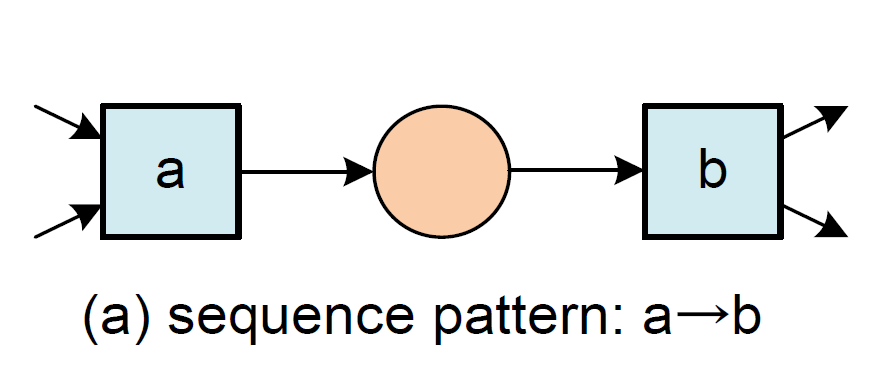
\includegraphics[width=0.5\textwidth]{capitolo 5/5 sequence pattern.png}
    \end{center}
    
    \subsection{XOR-Split Pattern}
    The XOR-split pattern is represented as \(a \rightarrow b\), \(a \rightarrow c\), and \(b \# c\), indicating that after activity \(a\), either \(b\) or \(c\) will follow, but not both.
    
    \begin{center}
        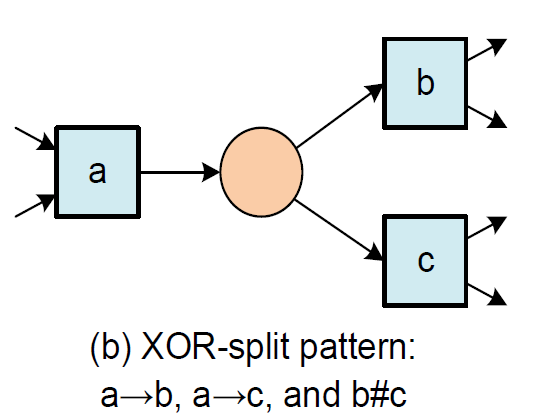
\includegraphics[width=0.5\textwidth]{capitolo 5/5 xor split.png}
    \end{center}
    
    \subsection{XOR-Join Pattern}
    The XOR-join pattern is represented as \(a \rightarrow c\), \(b \rightarrow c\), and \(a \# b\), meaning that activity \(c\) can be reached from either \(a\) or \(b\), but \(a\) and \(b\) are mutually exclusive.
    
    \begin{center}
        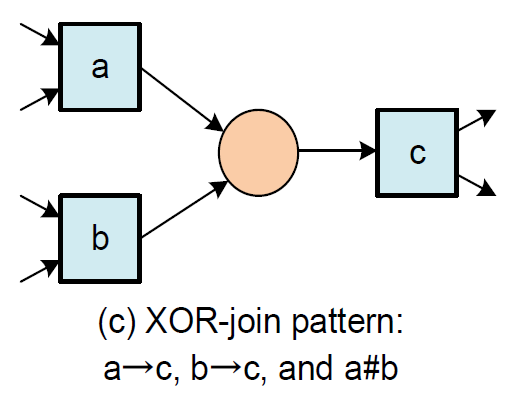
\includegraphics[width=0.5\textwidth]{capitolo 5/5 xor join.png}
    \end{center}
    
    \subsection{AND-Split Pattern}
    The AND-split pattern is represented as \(a \rightarrow b\), \(a \rightarrow c\), and \(b || c\), indicating that after activity \(a\), both \(b\) and \(c\) will occur in parallel.
    
    \begin{center}
        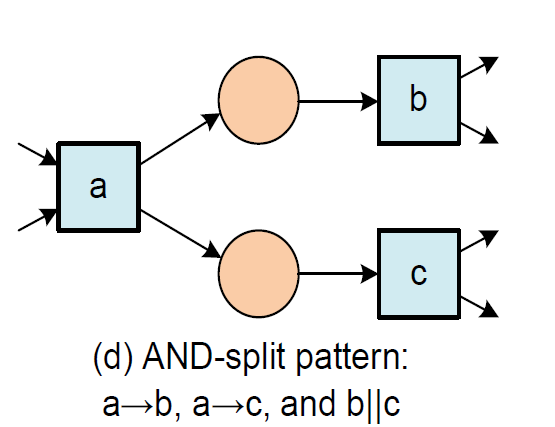
\includegraphics[width=0.5\textwidth]{capitolo 5/5 and split pattern.png}
    \end{center}
    
    \subsection{AND-Join Pattern}
    The AND-join pattern is represented as \(a \rightarrow c\), \(b \rightarrow c\), and \(a || b\), meaning that activity \(c\) occurs after both \(a\) and \(b\) have completed.
    
    \begin{center}
        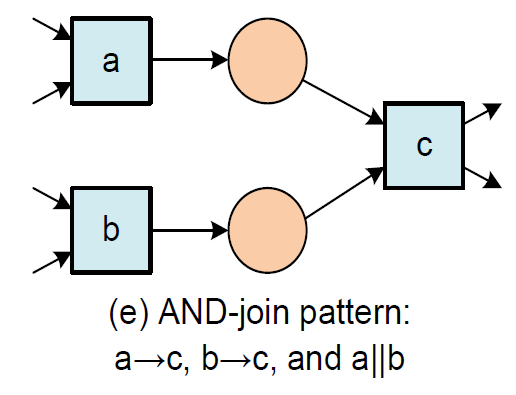
\includegraphics[width=0.5\textwidth]{capitolo 5/5 and join pattern.png}
    \end{center}
    
    \subsection{Summary of Patterns}
    The following image summarizes all the patterns described above:
    
    \begin{center}
        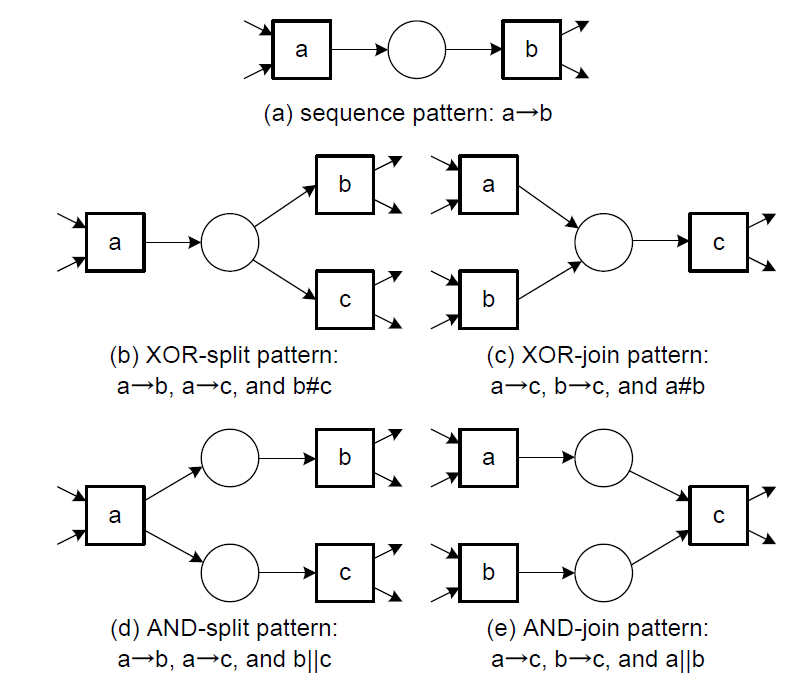
\includegraphics[width=\textwidth]{capitolo 5/5 recap pattern.png}
    \end{center}
    
    \section{Steps of the Alpha Algorithm}
    
    Given an event log \(L\) over a set of transitions \(T\) and trace $\sigma$, the Alpha Algorithm, $\alpha(L)$, defines a workflow model in the following steps:
    
    \begin{enumerate}
        \item Define the set \(T_L\) as the set of all transitions in \(L\): \[
        T_L = \{ t \in T \mid \exists \sigma \in L \text{ such that } t \in \sigma \}.
        \]
        \item Define the set of initial transitions \(T_I\) as those that are the first in some trace: \[
        T_I = \{ t \in T \mid \exists \sigma \in L \text{ such that } t = \text{first}(\sigma) \}.
        \]
        \item Define the set of final transitions \(T_O\) as those that are the last in some trace: \[
        T_O = \{ t \in T \mid \exists \sigma \in L \text{ such that } t = \text{last}(\sigma) \}.
        \]
        \item Calculate all pairs of transitions \( (A, B) \), where \(A\) and \(B\) are subsets of \(T_L\), such that every element of \(A\) is causally related to every element of \(B\), and the elements within \(A\) and \(B\) are independent of each other.
        \item Delete all non-maximal pairs from the set of pairs \( (A, B) \).
        \item For each remaining pair \( (A, B) \), define a place \(p(A, B)\) and connect it to the transitions in \(A\) and \(B\).
        \item Add an initial place connected to all start transitions in \(T_I\) and a final place connected to all end transitions in \(T_O\).
        \item Output the resulting Petri net, denoted as \( \alpha(L) = (P_L, T_L, F_L) \), where \(P_L\) is the set of places and \(F_L\) is the flow relation.
    \end{enumerate}
    
    \section{Limitations of the Alpha Algorithm}
    
    The Alpha Algorithm has several limitations:
    \begin{itemize}
        \item \textbf{Implicit places:} The algorithm may introduce places that do not correspond to meaningful behavior in the process. 
        \begin{center}
            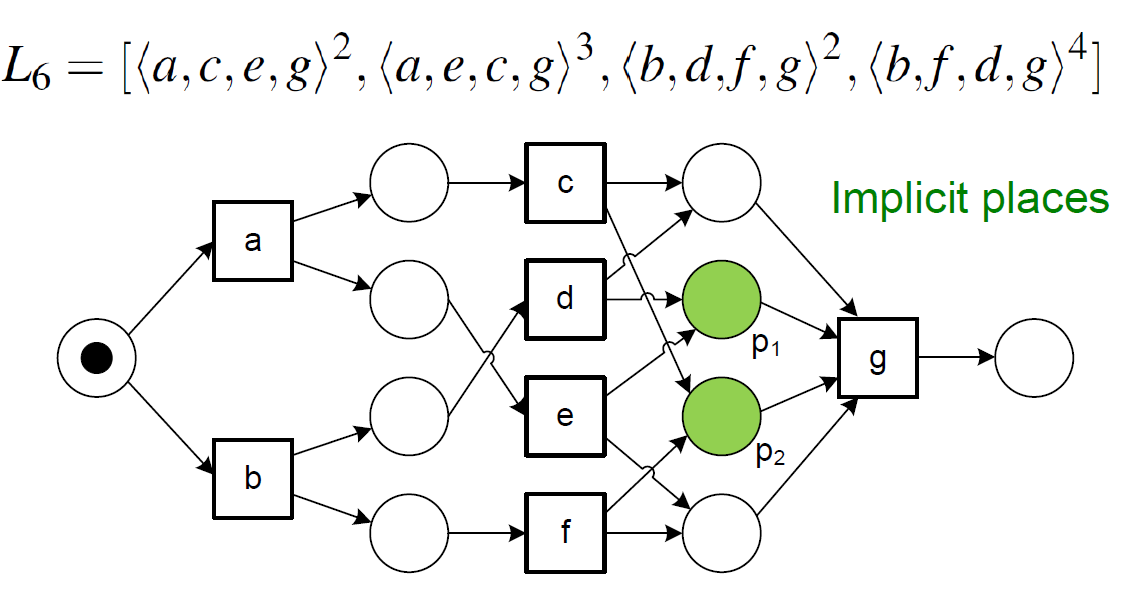
\includegraphics[width=\textwidth]{capitolo 5/5 limit 1 .png}
        \end{center}
        \item \textbf{Loops of length 1:} The algorithm struggles with loops of length 1, where a transition can fire multiple times in succession.
        \begin{center}
            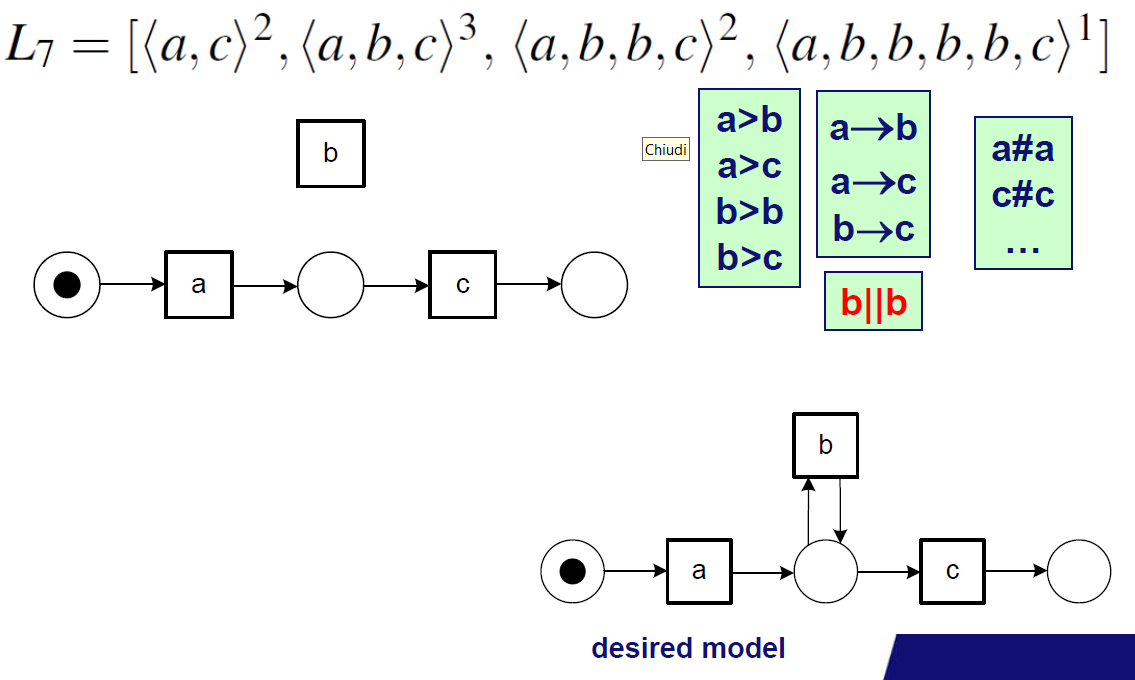
\includegraphics[width=\textwidth]{capitolo 5/5 limit 2.png}
        \end{center}
        \item \textbf{Loops of length 2:} Similarly, the algorithm has difficulty handling loops of length 2, where two transitions alternate repeatedly.
        \begin{center}
            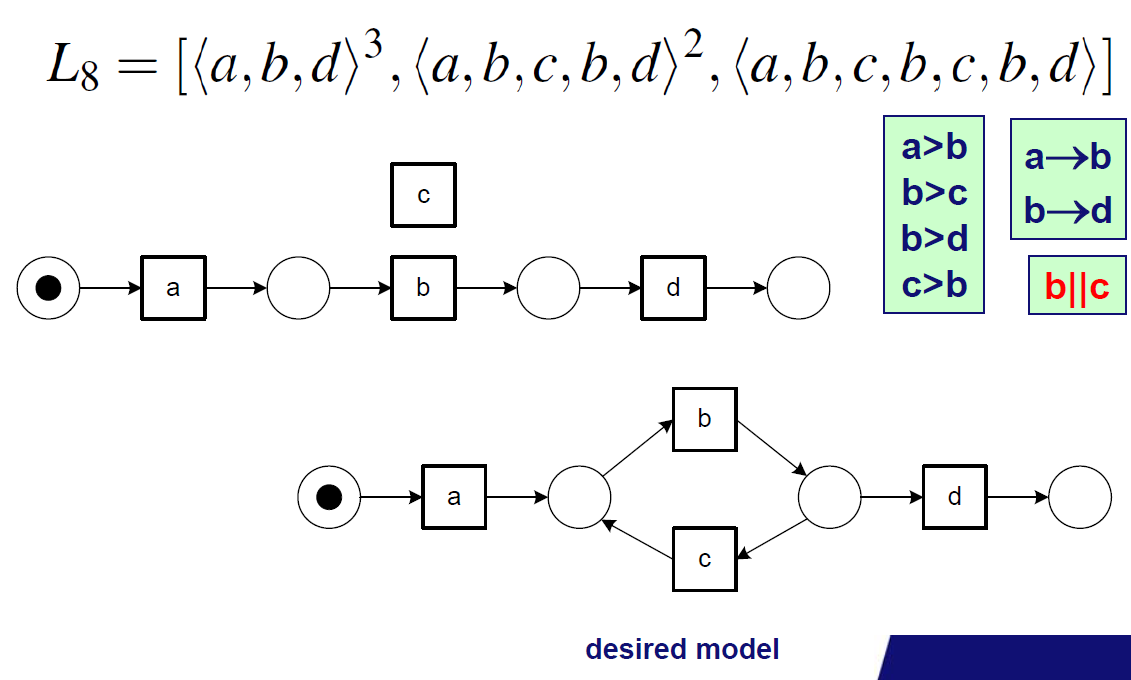
\includegraphics[width=\textwidth]{capitolo 5/5 limit 3.png}
        \end{center}
        \item \textbf{Non-local dependencies:} The algorithm cannot discover non-local dependencies, where the behavior of a transition depends on events that occurred much earlier in the process.
        \begin{center}
            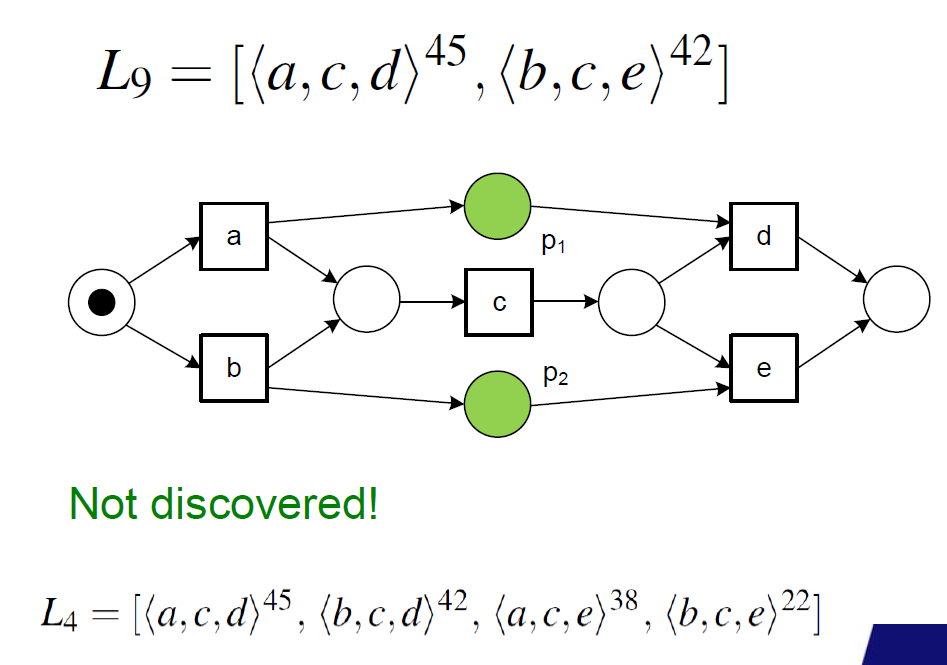
\includegraphics[width=\textwidth]{capitolo 5/5 limit 4.png}
        \end{center}
        \item Some bias is needed because we have to exclude some behaviour such as two equal transitions firing one after the other. 
        \begin{center}
            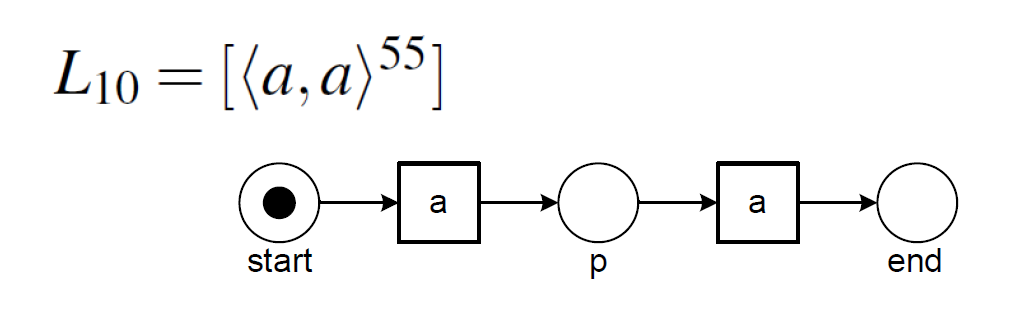
\includegraphics[width=\textwidth]{capitolo 5/5 limit 5.png}
        \end{center}
        \item \textbf{Noise and incompleteness:} Event logs may contain noise, or rare, unrepresentative behavior. Moreover, incomplete logs may not capture all the possible variations of the process. It has to be generalised. 
    \end{itemize}
       
    
    \section{Flower Model}
    
    The \textbf{Flower Model} is an extreme example of an over-generalized process model. It allows any activity to occur at any time, in any order, and still result in a valid process execution. While this model has perfect fitness (i.e., it can replay all the observed traces), it lacks precision and generalization.
    
    \begin{center}
        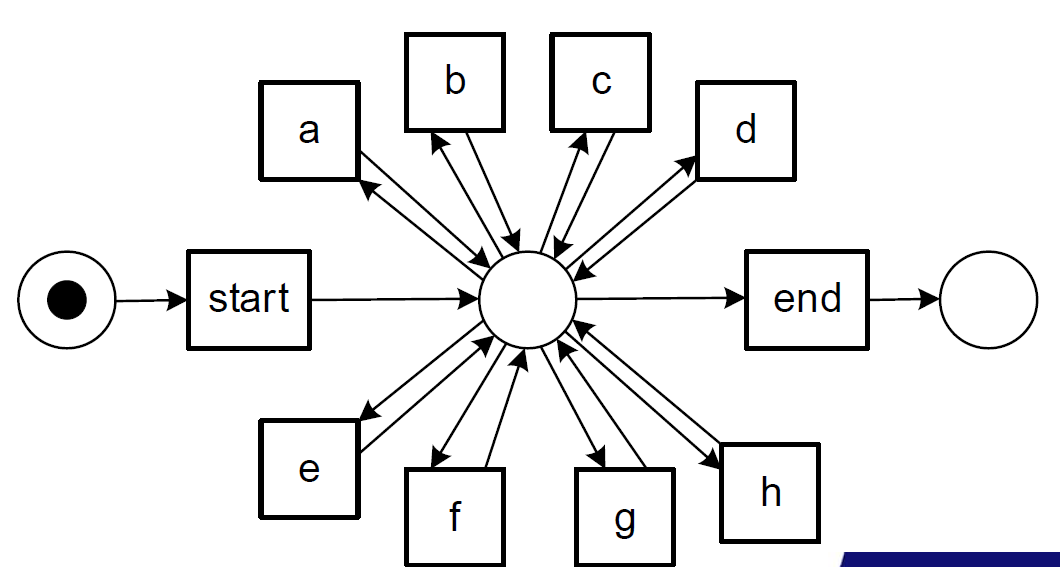
\includegraphics[width=0.5\textwidth]{capitolo 5/5 flower model.png} % Insert image of Flower Model
    \end{center}
    
    \section{Balancing Four Forces in Process Models}
    
    To create an optimal process model, four key forces must be balanced:
    \begin{itemize}
        \item \textbf{Fitness:} The ability of the model to explain the observed behavior in the event log.
        \item \textbf{Generalization:} The ability of the model to handle unobserved but possible behavior, avoiding overfitting.
        \item \textbf{Precision:} The model should not allow behavior that is not present in the log, avoiding underfitting.
        \item \textbf{Simplicity:} The model should be as simple as possible while still capturing the essential behavior of the process.
    \end{itemize}
    
    
    \section{Example: Model Comparison}
    
    Consider the following example of process discovery using a log with multiple traces. The four models below are evaluated based on their \textit{fitness}, \textit{generalization}, \textit{precision}, and \textit{simplicity}.
    
    
    \subsection{Model N1}
    Model N1 has high fitness, precision, generalization, and simplicity. It is an ideal model that balances all four forces well.
    \begin{center}
        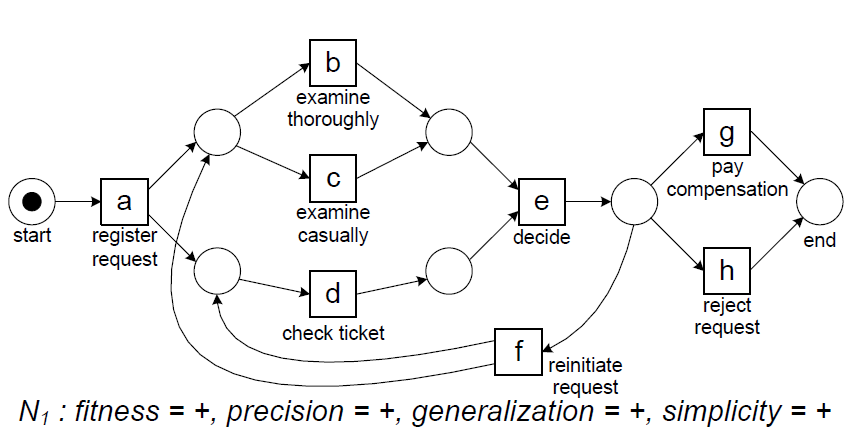
\includegraphics[width=0.5\textwidth]{capitolo 5/5 n1.png} % Insert image of model comparison
    \end{center}
    \subsection{Model N2}
    Model N2 has high precision and simplicity but lacks generalization and fitness. This model may overfit to the observed traces, excluding potential valid behaviors.
    \begin{center}
        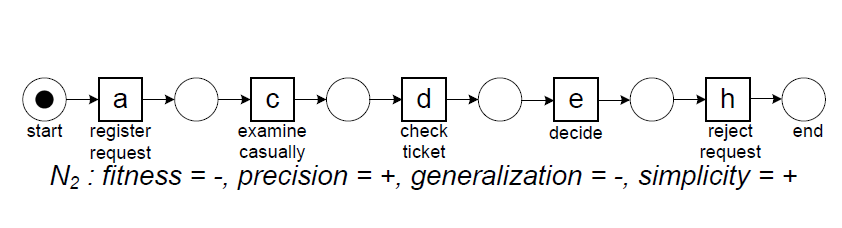
\includegraphics[width=0.5\textwidth]{capitolo 5/5 n2.png} % Insert image of model comparison
    \end{center}
    \subsection{Model N3}
    Model N3 has high fitness and generalization but low precision. This indicates that the model allows too much flexibility, potentially enabling behavior that is not observed in the event log.
    \begin{center}
        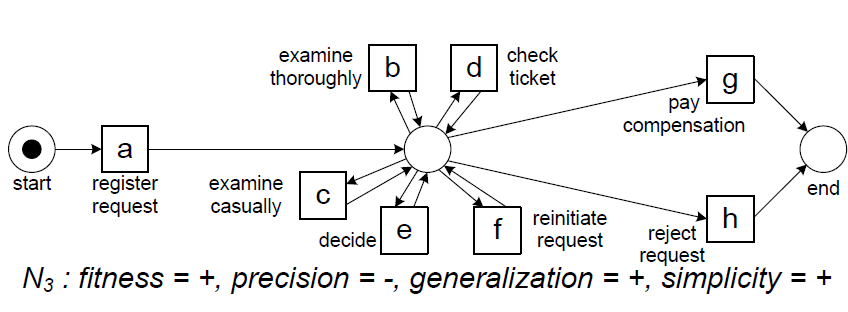
\includegraphics[width=0.5\textwidth]{capitolo 5/5 n3.png} % Insert image of model comparison
    \end{center}
    \subsection{Model N4}
    Model N4 has high fitness and precision but poor generalization. While it accurately reflects the observed traces, it may not handle new or unseen behaviors effectively.
    \begin{center}
        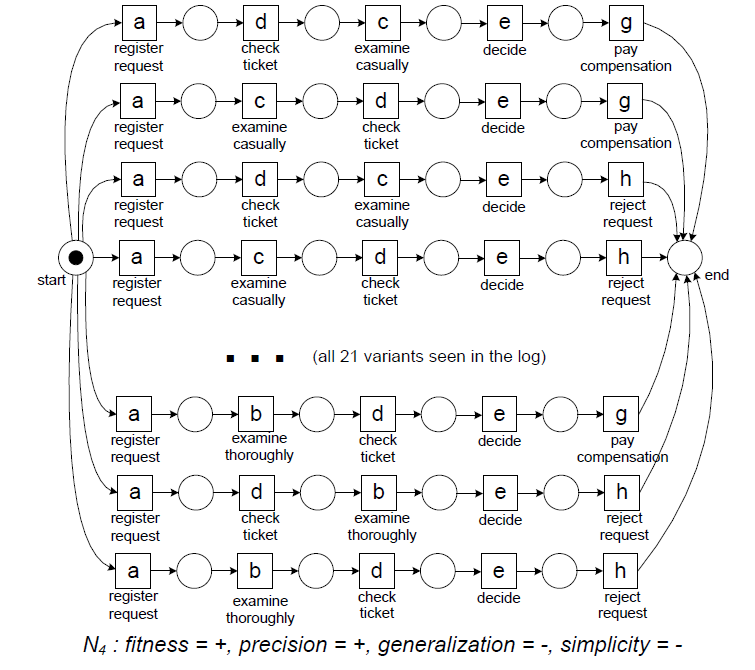
\includegraphics[width=0.5\textwidth]{capitolo 5/5 n4.png} % Insert image of model comparison
    \end{center}

\chapter{Advanced Process Discovery: Dependency Measure, Causal Nets, and Heuristic Miner}
To improve our Petri net models, we need to address certain limitations. Initially, we notice several problems:
\begin{itemize}
    \item The current notation does not capture the \textbf{frequency} of events, which means it treats rare events the same as frequent ones.
    \item There is no clear distinction between \textbf{causal relationships}, such as AND splits and XOR splits, in the coverability graph.
\end{itemize}
To address these issues, we introduce the \textbf{dependency measure}, which allows us to quantify the dependency between activities and account for noise.

\section{Dependency Measure}

The \textbf{dependency measure} quantifies the strength of the dependency between two activities \(a\) and \(b\). The formula is as follows:
\begin{equation}
    |a \Rightarrow_L b| =
\begin{cases}
\frac{|a >_L b| - |b >_L a|}{|a >_L b| + |b >_L a| + 1} \hspace{3mm} a \neq b \\
\frac{|a >_L a|}{|a >_L a|+1} \hspace{3mm} a = b
\end{cases}
\end{equation}

Where:
\begin{itemize}
    \item \(|a >_L b|\) represents the number of times \(a\) is directly followed by \(b\),
    \item \(|b >_L a|\) represents the number of times \(b\) is directly followed by \(a\),
    \item The addition of \(+1\) in the denominator prevents division by zero in cases where there is no relationship between \(a\) and \(b\).
\end{itemize}

This measure ranges from \(-1\) to \(1\), where:
\begin{itemize}
    \item If \(|a >_L b| \gg |b >_L a|\), then \(a \Rightarrow_L b \approx 1\), indicating a strong causal relationship.
    \item If \(|a >_L b| = |b >_L a|\), then \(a \Rightarrow_L b = 0\), meaning no clear dependency.
    \item If \(|b >_L a| \gg |a >_L b|\), then \(a \Rightarrow_L b \approx -1\), indicating reverse causality.
\end{itemize}

The dependency measure also filters out noise, as arcs with low dependency values are considered less relevant.

\section{Causal Nets (C-nets)}

To further address the limitations of Petri nets, we introduce \textbf{Causal nets (C-nets)}. C-nets are more expressive and allow us to explicitly model how transitions occur. In a C-net, every activity requires an \textbf{obligation} (similar to tokens) for activation. Once activated, the activity consumes its input obligations and produces new ones for subsequent activities.

\begin{center}
    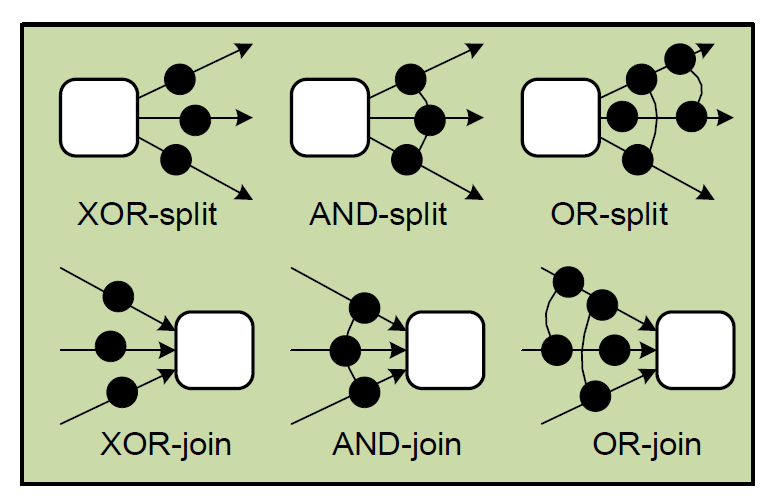
\includegraphics[width=0.5\textwidth]{capitolo 6/6 cnet notation.png} % Insert image of Causal Net patterns
\end{center}

\subsection{Binding Obligations}
In C-nets, obligations work similarly to tokens in Petri nets. When an activity is activated, it "burns" its input obligations and generates new output obligations, as shown below:

\begin{center}
    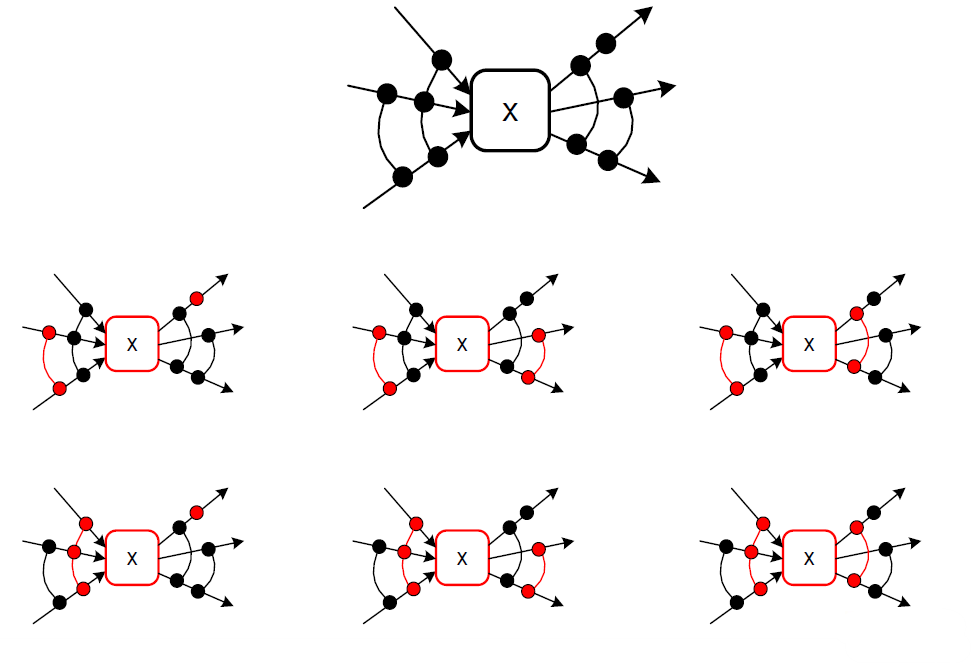
\includegraphics[width=0.5\textwidth]{capitolo 6/6 binding.png} % Insert image of binding example
\end{center}

From any Causal net, it is possible to derive a Petri net, and vice versa. Each \textbf{invisible transition} in the Petri net can be treated as a different binding in the C-net.

\begin{center}
    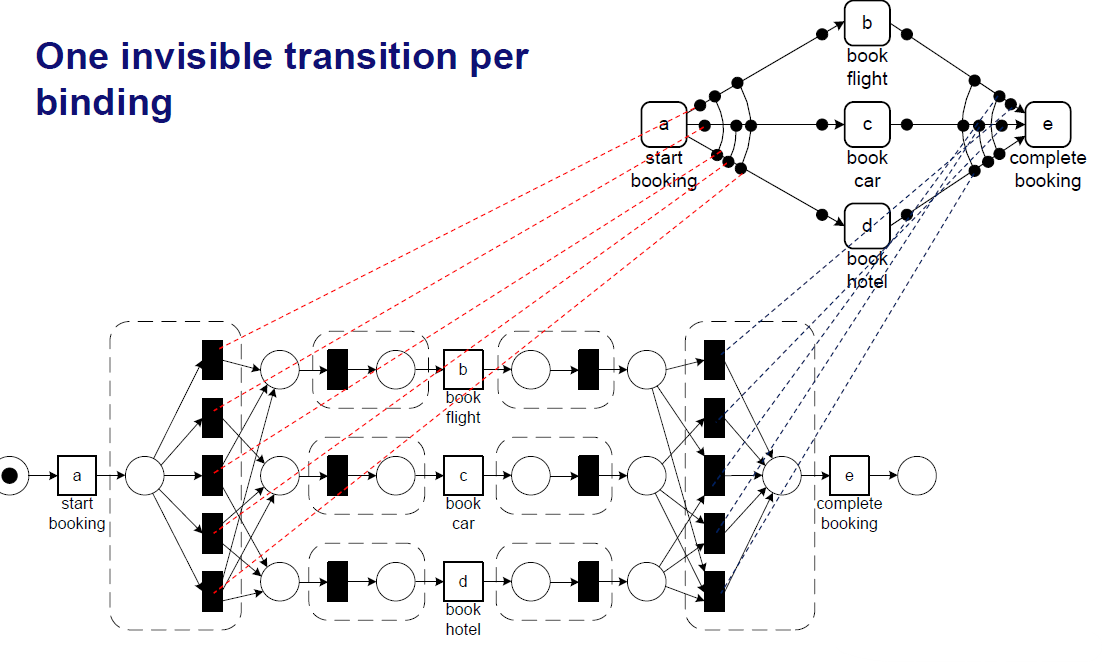
\includegraphics[width=0.8\textwidth]{capitolo 6/6 cnet to petri.png} % Insert image showing conversion from C-net to Petri net
\end{center}

However, the C-net model is not yet perfect and might not always be sound.

\section{Heuristic Miner}

The \textbf{Heuristic Miner} introduces a different approach. Instead of solely focusing on direct causality, it considers the frequency of activities. The steps are:
\begin{enumerate}
    \item Given an event log, build a \textbf{dependency graph}.
    \item Learn where the splits and joins are (AND/XOR).
    \item Visualize them and provide the graph to a tool.
    \item The tool counts how often certain sets of inputs and outputs appear, allowing it to calculate the frequency of bindings and select the most frequent ones.
\end{enumerate}

The \textbf{best guess} approach is used, meaning the miner does not analyze end-to-end traces but rather makes decisions based on local observations.

\subsection{Example: Infinite Window}
Let's explain the process of constructing initial and final bindings using the infinite window approach. In this example:
\begin{center}
    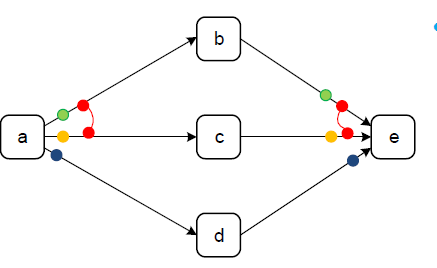
\includegraphics[width=0.5\textwidth]{capitolo 6/6 infinite window.png} % Insert image for Infinite Window example
\end{center}

\begin{itemize}
    \item Activity \(A\) is sometimes followed by \(B\) and \(C\) but not by \(D\). This occurs in the traces \(\langle a, b, c, e \rangle\) and \(\langle a, c, b, e \rangle\).
    \item Therefore, this suggests an \textbf{AND-split} of \(A\) with \(B\) and \(C\) (red dots).
    \item Activity \(A\) is sometimes followed by only \(E\), as seen in the trace \(\langle a, e \rangle\). However, this is ignored as there is no significant dependency. 
    \item Activity \(A\) is sometimes followed by \(B\) but not by \(C\) or \(D\), as shown in the trace \(\langle a, b, e \rangle\) (green dot).
    \item Activity \(A\) is sometimes followed by \(C\) but not by \(B\) or \(D\), as shown in the trace \(\langle a, c, e \rangle\) (yellow dot).
    \item Finally, \(A\) is sometimes followed by \(D\) but not by \(B\) or \(C\), in traces like \(\langle a, d, ..., d, e \rangle\) (blue dot).
\end{itemize}

This results in the following structure:
\[
A \rightarrow B, C, D
\]

In this example, we focus on how activity \(E\) behaves:
\begin{itemize}
    \item Activity \(E\) is sometimes preceded by \(B\) and \(C\) but not by \(D\), as in the traces \(\langle a, b, c, e \rangle\) and \(\langle a, c, d, e \rangle\), indicating an \textbf{OR-join} with \(B\) and \(C\) (red dots).
    \item Sometimes \(E\) is preceded only by \(A\), as in \(\langle a, e \rangle\), which is ignored due to lack of dependency.
    \item \(E\) is also preceded by \(B\) but not by \(C\) or \(D\), as seen in \(\langle a, b, e \rangle\) (green dot).
    \item Similarly, \(E\) is preceded by \(C\) but not by \(B\) or \(D\), as in \(\langle a, c, e \rangle\) (yellow dot).
    \item Finally, \(E\) is preceded by \(D\) but not by \(B\) or \(C\), in traces like \(\langle a, d, ..., d, e \rangle\) (blue dot).
\end{itemize}

This produces the structure:
\[
E \rightarrow B, C, D
\]



\section{Region Miner (use slides for better images)}

Another advanced model is the \textbf{Region Miner}. The goal is to learn a transition system from an event log using state abstraction, then transform it into a Petri net.

The \textbf{transition system} allows us to understand the past and future of a given state. We use a schema, represented by black dots, to abstract states.

\begin{center}
    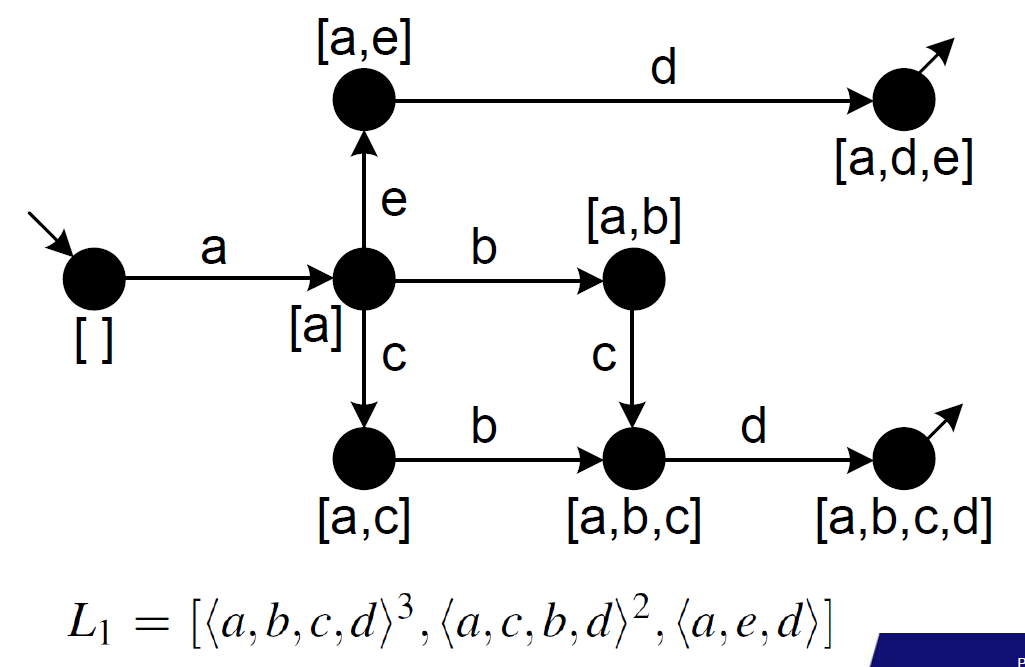
\includegraphics[width=0.5\textwidth]{capitolo 6/6 region miner scheme.png} % Insert image showing transition system abstraction
\end{center}

From the transition system, we can move to a Petri net by delimiting regions. A \textbf{region} corresponds to a place in the Petri net. A region is a set of states such that:
\begin{itemize}
    \item If a transition exits the region, then all transitions with the same label exit the region.
    \item If a transition enters the region, then all transitions with the same label enter the region.
    \item Events that do not enter or exit the region do not cross it.
\end{itemize}

\begin{center}
    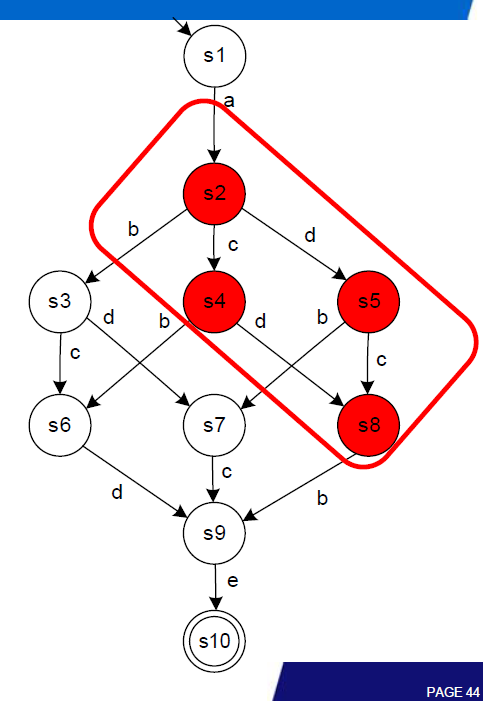
\includegraphics[width=0.5\textwidth]{capitolo 6/6 region 1.png} % Insert image showing region definition
\end{center}

\subsection{Minimal Regions}
We aim to extract the \textbf{minimal regions}, which are regions that do not contain other regions within them. Additionally:
\begin{itemize}
    \item The set \(S\) of all states and the empty set are \textbf{trivial regions}.
    \item If \(r\) is a region, then \(S \setminus r\) is also a region.
    \item If \(r_0\) and \(r_1\) are regions, and \(r_0 \subseteq r_1\), then \(r_1 \setminus r_0\) is a region.
\end{itemize}

\begin{center}
    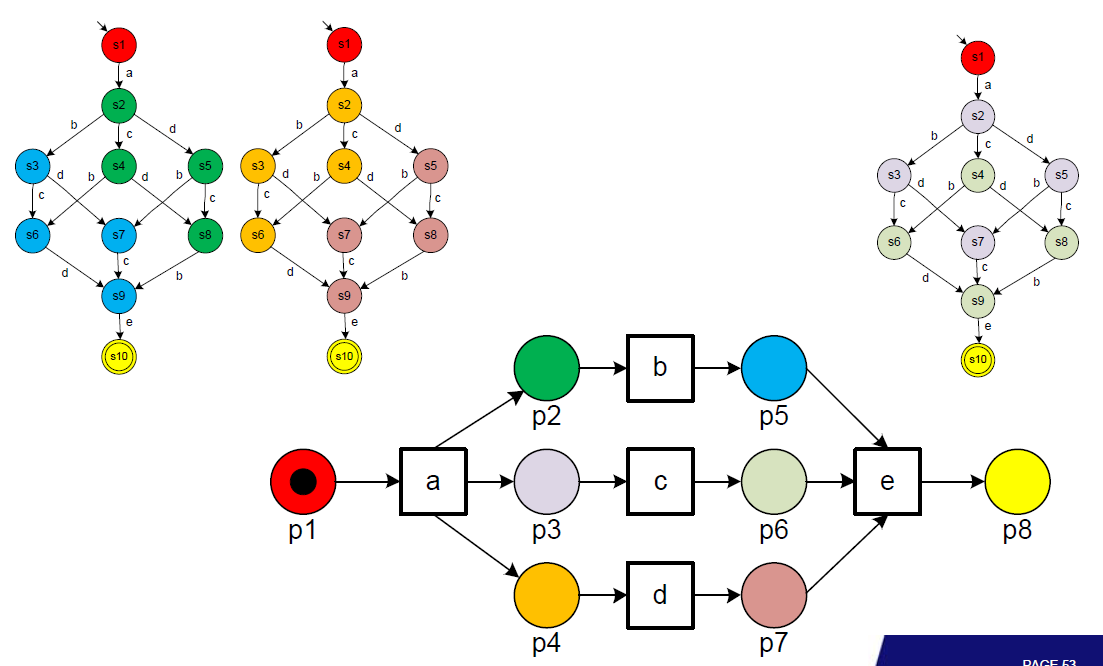
\includegraphics[width=0.8\textwidth]{capitolo 6/6 region 2.png} % Insert image showing minimal region example
\end{center}

\section{Algorithm for Constructing a Petri Net from a Transition System}

The algorithm to generate a Petri net from a transition system is as follows:
\begin{enumerate}
    \item For each event in the transition system, generate a transition in the Petri net.
    \item Compute the minimal non-trivial regions.
    \item For each minimal region, generate a place in the Petri net.
    \item Add corresponding arcs: post-regions as output places and pre-regions as input places.
    \item Add tokens to places that correspond to regions containing the initial state.
\end{enumerate}

\section{Conclusion}
Through advanced process discovery techniques like dependency measures, Causal nets, and region miners, we can construct more refined process models that account for frequency, noise, and complex dependencies. However, challenges like soundness and overfitting remain, and the selection of the appropriate discovery method depends on the specific use case.



\chapter{Strassen Matrix Multiplication}
    
    Before introducing Strassen's method, let's examine standard matrix multiplication, called \textbf{Square-Matrix-Multiplication (SMMR)}. Given two \(n \times n\) matrices \(A\) and \(B\), we want to compute their product \(C = A \times B\).
    
    \subsection{Standard Matrix Multiplication (SMMR)}
    1. Divide matrices \(A\) and \(B\) as follows:
       \[
       A = \begin{bmatrix} A_{11} & A_{12} \\ A_{21} & A_{22} \end{bmatrix}, \quad B = \begin{bmatrix} B_{11} & B_{12} \\ B_{21} & B_{22} \end{bmatrix}
       \]
       
    2. Each element of \(C\) is computed as:
       \[
       C = A \times B = \begin{bmatrix} C_{11} & C_{12} \\ C_{21} & C_{22} \end{bmatrix}
       \]
       where
       \[
       C_{11} = A_{11} B_{11} + A_{12} B_{21}, \quad C_{12} = A_{11} B_{12} + A_{12} B_{22}
       \]
       \[
       C_{21} = A_{21} B_{11} + A_{22} B_{21}, \quad C_{22} = A_{21} B_{12} + A_{22} B_{22}
       \]
    
    This method requires 8 recursive multiplications for each submatrix.
    
    \subsection{Recursive SMMR Algorithm}
    
    \begin{verbatim}
    def SMMR(A, B):
        n = len(A)  # Number of rows in A
        C = [[0] * n for _ in range(n)]  # Initialize nxn matrix C with zeros
        
        if n == 1:
            C[0][0] = A[0][0] * B[0][0]
        else:
            # Partition matrices A, B, and C as described
            C11 = SMMR(A11, B11) + SMMR(A12, B21)
            C12 = SMMR(A11, B12) + SMMR(A12, B22)
            C21 = SMMR(A21, B11) + SMMR(A22, B21)
            C22 = SMMR(A21, B12) + SMMR(A22, B22)
            
            # Combine results into matrix C (requires additional merging steps in practice)
        
        return C
    \end{verbatim}
    
    \subsection{Complexity Analysis of SMMR}
    
    Dividing each matrix into four \( \frac{n}{2} \times \frac{n}{2} \) submatrices requires 8 multiplications. Assuming each submatrix has \( \left(\frac{n}{2}\right)^2 = \frac{n^2}{4} \) entries, we derive the recurrence:
    \[
    T(n) = \begin{cases} 
          \Theta(1) & \text{if } n = 1 \\
          8T\left(\frac{n}{2}\right) + \Theta(n^2) & \text{if } n > 1 
       \end{cases}
    \]
    
    The height of the recursion tree is \(\log_2 n\), and the total number of leaves is \(n^{\log_2 8} = n^3\), leading to:
    
    
    \section{Strassen's Algorithm}
    
    Strassen's algorithm presents a clever approach to improve the efficiency of matrix multiplication, specifically for large matrices. Although it is challenging to apply this algorithm beyond the context of matrix multiplication, studying it is highly useful for understanding the principles of recursion and complexity analysis in algorithms. 
    
    \subsection{Standard Recursive Matrix Multiplication}
    As previously discussed, multiplying two matrices \(A\) and \(B\) can be formulated as a recursive problem. Each matrix is divided into four \( \frac{n}{2} \times \frac{n}{2} \) submatrices, and recursive calls are made until we reach matrices of size \(1 \times 1\), where the multiplications are performed directly. This standard approach yields a time complexity of \(\Theta(n^3)\).
    
    \subsection{Overview of Strassen's Algorithm}
    Strassen’s algorithm reduces the complexity of matrix multiplication by leveraging specific combinations of additions and multiplications. It consists of four main steps:
    \begin{enumerate}
        \item Divide matrices \(A\) and \(B\) into \( \frac{n}{2} \times \frac{n}{2} \) submatrices, similar to the standard approach.
        \item Construct 10 intermediate matrices \( S_1, S_2, \dots, S_{10} \) of size \( \frac{n}{2} \times \frac{n}{2} \), each representing specific sums or differences of the submatrices of \(A\) and \(B\). These combinations are carefully chosen to optimize the calculation process, as we will see shortly. This step has a complexity of \(\Theta(n^2)\).
        \item Using the submatrices from steps 1 and 2, compute 7 product matrices \( P_1, P_2, \dots, P_7 \), each of size \( \frac{n}{2} \times \frac{n}{2} \), by recursively applying the Strassen algorithm.
        \item Finally, construct the resulting submatrices \( C_{11}, C_{12}, C_{21}, C_{22} \) for the product matrix \(C\), using the product matrices \(P_i\). This step also has a complexity of \(\Theta(n^2)\).
    \end{enumerate}
    
    The key improvement in Strassen's algorithm lies in reducing the number of recursive multiplications from 8 to 7, which reduces the overall complexity.
    
    \subsection{Detailed Steps of Strassen’s Algorithm}
    \subsubsection*{Step 1: Divide Matrices}
    This step involves partitioning \(A\) and \(B\) as:
    \[
    A = \begin{bmatrix} A_{11} & A_{12} \\ A_{21} & A_{22} \end{bmatrix}, \quad B = \begin{bmatrix} B_{11} & B_{12} \\ B_{21} & B_{22} \end{bmatrix}
    \]
    
    \subsubsection*{Step 2: Construct Intermediate Sum Matrices}
    Define the following intermediate matrices:
    \[
    \begin{aligned}
        S_1 &= B_{12} - B_{22}, \\
        S_2 &= A_{11} + A_{12}, \\
        S_3 &= A_{21} + A_{22}, \\
        S_4 &= B_{21} - B_{11}, \\
        S_5 &= A_{11} + A_{22}, \\
        S_6 &= B_{11} + B_{22}, \\
        S_7 &= A_{12} - A_{22}, \\
        S_8 &= B_{21} + B_{22}, \\
        S_9 &= A_{11} - A_{21}, \\
        S_{10} &= B_{11} + B_{12}.
    \end{aligned}
    \]
    
    \subsubsection*{Step 3: Compute Product Matrices}
    Calculate the seven product matrices as follows:
    \[
    \begin{aligned}
        P_1 &= A_{11} \cdot S_1, \\
        P_2 &= S_2 \cdot B_{22}, \\
        P_3 &= S_3 \cdot B_{11}, \\
        P_4 &= A_{22} \cdot S_4, \\
        P_5 &= S_5 \cdot S_6, \\
        P_6 &= S_7 \cdot S_8, \\
        P_7 &= S_9 \cdot S_{10}.
    \end{aligned}
    \]
    
    \subsubsection*{Step 4: Construct Final Product Matrix \(C\)}
    Using the product matrices \(P_1, P_2, \dots, P_7\), construct the final submatrices of \(C\):
    \[
    \begin{aligned}
        C_{11} &= P_5 + P_4 - P_2 + P_6, \\
        C_{12} &= P_1 + P_2, \\
        C_{21} &= P_3 + P_4, \\
        C_{22} &= P_5 + P_1 - P_3 - P_7.
    \end{aligned}
    \]
    The final product matrix \(C\) is given by:
    \[
    C = \begin{bmatrix} C_{11} & C_{12} \\ C_{21} & C_{22} \end{bmatrix}
    \]
    
    \subsection{Complexity Analysis of Strassen's Algorithm}
    Despite the algorithm's complexity in terms of individual operations, it reduces the number of multiplications needed, which decreases the overall complexity. Strassen's algorithm achieves a time complexity of:
    \[
    \Theta(n^{\log_2 7}) \approx \Theta(n^{2.8073})
    \]
    This represents a significant improvement over the standard matrix multiplication complexity of \(\Theta(n^3)\).

\chapter{Mining additional perspectives}

\section{Introduction}

Until now, process mining has focused primarily on events recorded in an event log. However, significant insights can also be derived from examining \textbf{who} performs specific tasks or activities. This introduces new perspectives into the process mining, such as the resource, data, and time perspectives.

\subsection{Preprocessing and Filtering}
Before analyzing the event logs, it is essential to pre-process and filter the data to ensure its quality. This includes:
\begin{itemize}
    \item Removing irrelevant or noisy events,
    \item Organizing the data for visualization and analysis.
\end{itemize}

\section{Visualizing Data: Dotted Charts and Helicopter View}

\subsection{Dotted Chart}
A \textbf{dotted chart} is a graphical representation of event logs:
\begin{itemize}
    \item The \textbf{x-axis} represents timestamps,
    \item The \textbf{y-axis} represents trace numbers.
\end{itemize}

This chart helps to visualize how individual customers or cases progress over time. For example:
\begin{itemize}
    \item Denser lines indicate frequent activities,
    \item Sparse dots indicate rare or exceptional events.
\end{itemize}


\subsection{Helicopter View}
By varying symbols, colors and shapes in the dotted chart, a \textbf{helicopter view} can be created, providing insight into trends and variations in activities over time.
\begin{center}
    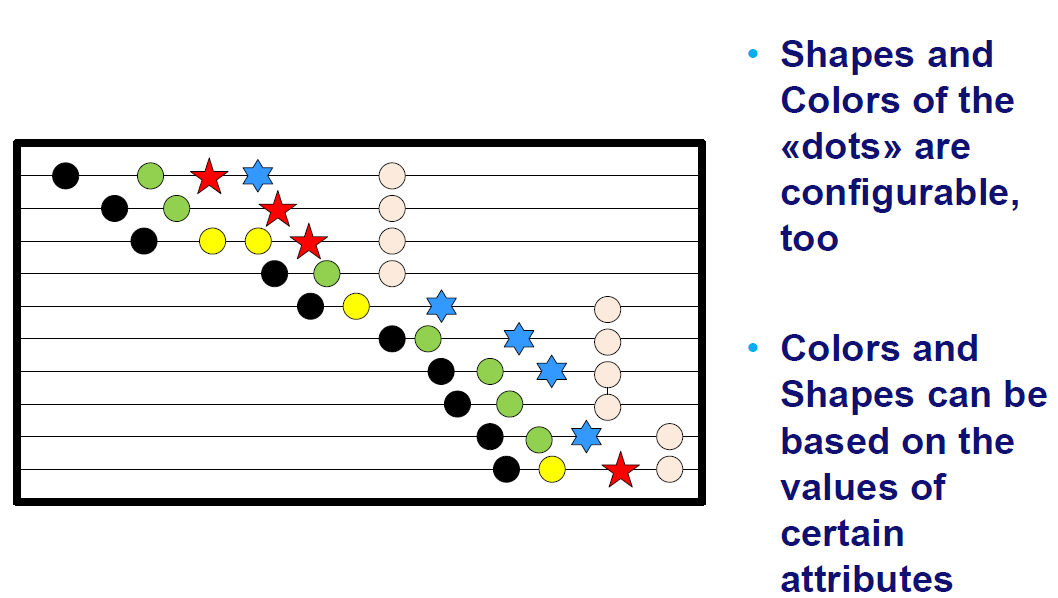
\includegraphics[width=0.7\textwidth]{capitolo 8/slide10.png}
\end{center}
For example:
\begin{itemize}
    \item Constant arrival rates,
    \item Patterns of grouped cancellations,
    \item Time-dependent changes in activity density,
    \item The amount of work each member do.
\end{itemize}
\begin{center}
    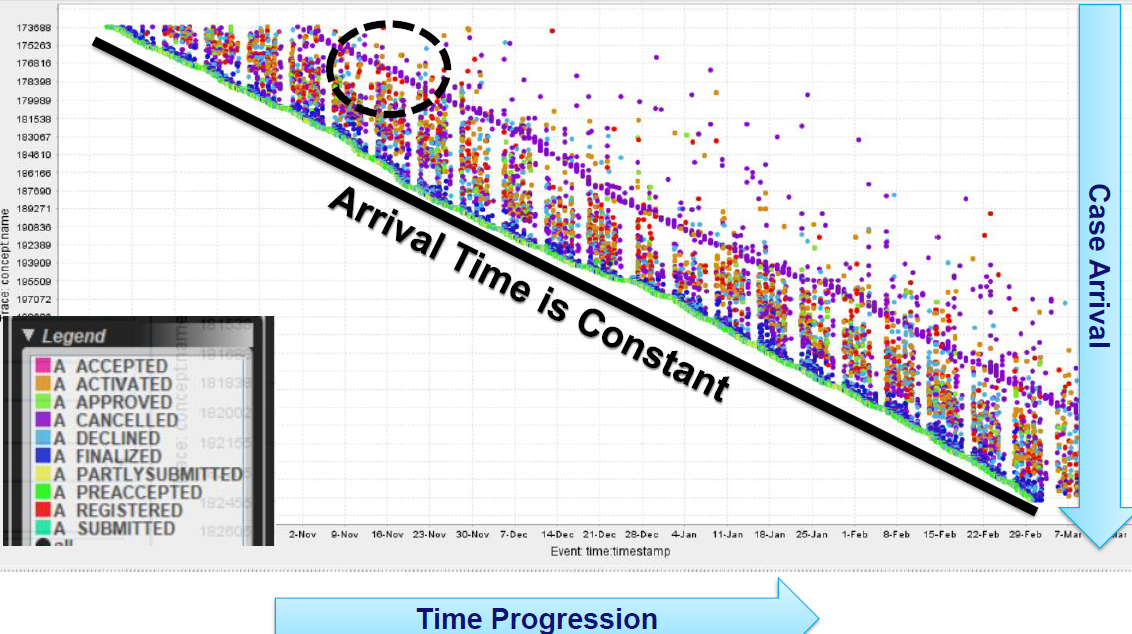
\includegraphics[width=0.7\textwidth]{capitolo 8/slide11.png}
\end{center}

\begin{center}
    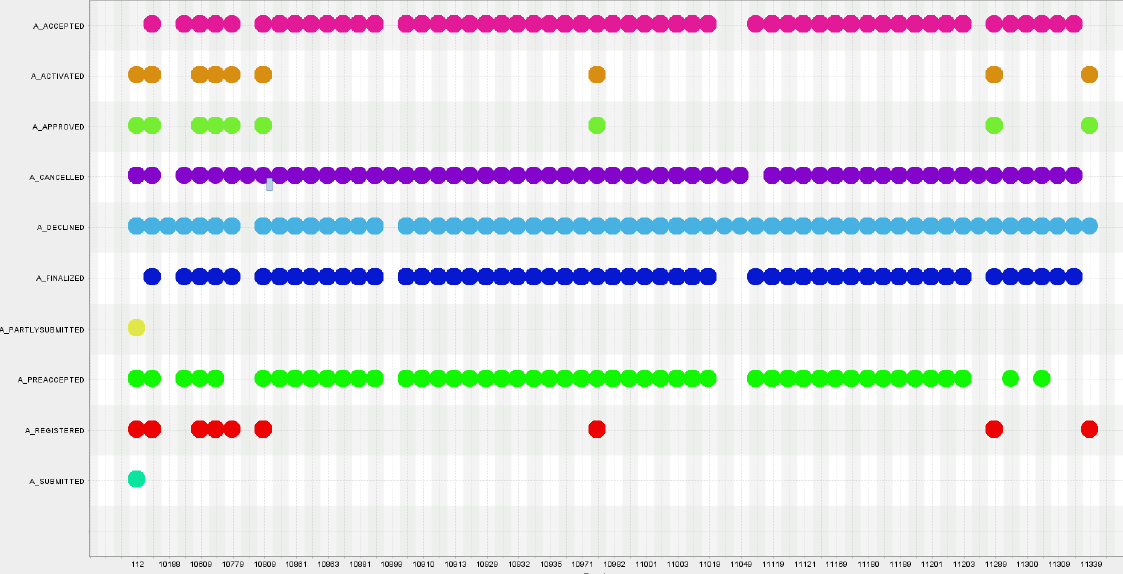
\includegraphics[width=0.7\textwidth]{capitolo 8/slide 14.png}
\end{center}

\section{Enhancing Petri Nets with Additional Perspectives}

\subsection{Resource Perspective: Organizational Mining}
The \textbf{organizational perspective} focuses on understanding people, machines, and organizational structures, such as:
\begin{itemize}
    \item Roles (e.g., manager, assistant),
    \item Departments,
    \item Work distribution among resources.
\end{itemize}

A \textbf{resource-activity matrix} records how often specific resources perform particular activities. For example:
\begin{itemize}
    \item Activity \(a\) is performed \(0.3\) times by Pete, \(0.5\) times by Mike, and \(0.2\) times by Ellen.
    \item Activities \(e\) and \(f\) are performed exclusively by Sara, often more than once per case.
\end{itemize}
\begin{center}
    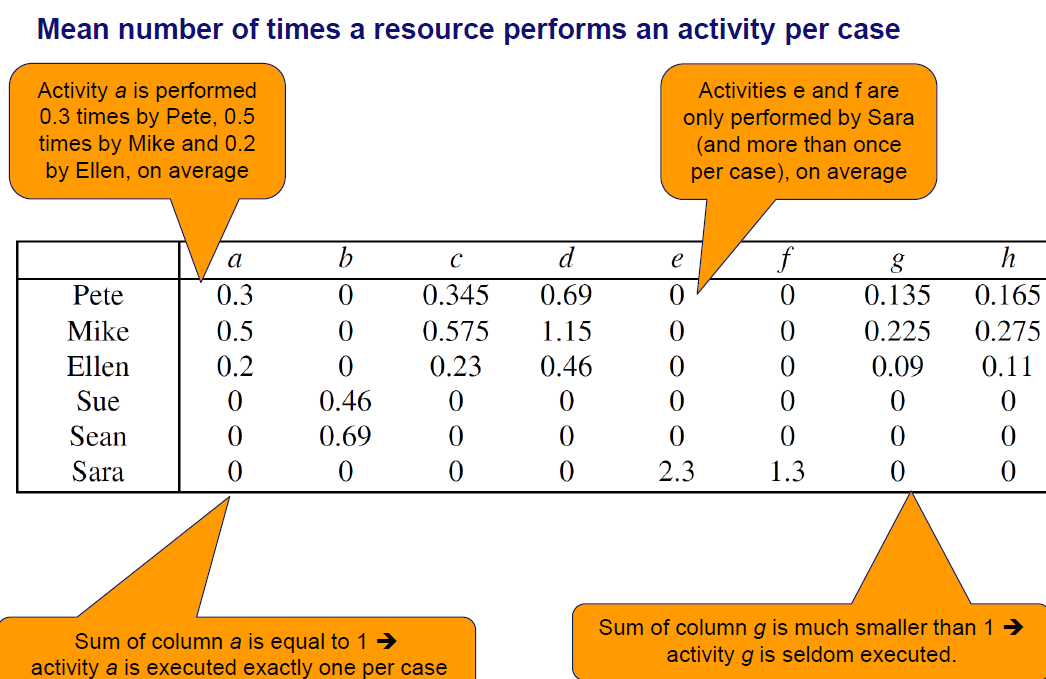
\includegraphics[width=0.7\textwidth]{capitolo 8/slide20.png}
\end{center}

Rows in the resource-activity matrix can be clustered to group resources with similar roles. Labels such as "manager," "expert," or "assistant" can be arbitrarily assigned to these clusters.

\subsection{Social Network Analysis}
Social networking techniques can visualize relationships between groups or individuals:
\begin{itemize}
    \item Nodes represent resources or roles,
    \item Arcs represent interactions (e.g., handover of work).
\end{itemize}
The size of nodes and the thickness of the arcs depend on the weight of entities and relationships, respectively.

\begin{center}
    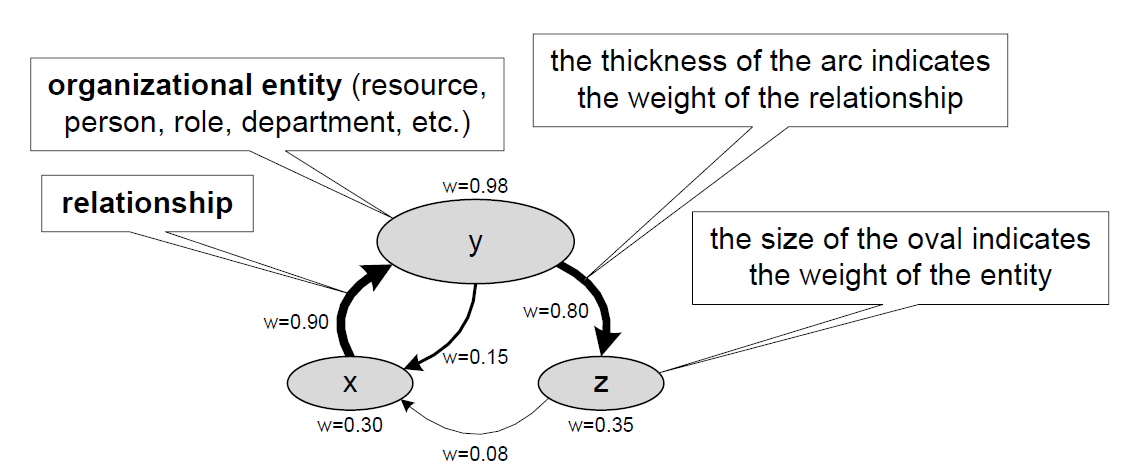
\includegraphics[width=0.7\textwidth]{capitolo 8/slide24.png}
\end{center}

\subsection{Handover of Work}
The \textbf{handover of work} represents the transfer of responsibility between resources. A direct or eventual dependency exists if:
\begin{itemize}
    \item Activity \(a_1\) is followed by \(a_2\),
    \item Or \(a_1\) indirectly influences \(a_2\) through intermediate activities.
\end{itemize}
\begin{center}
    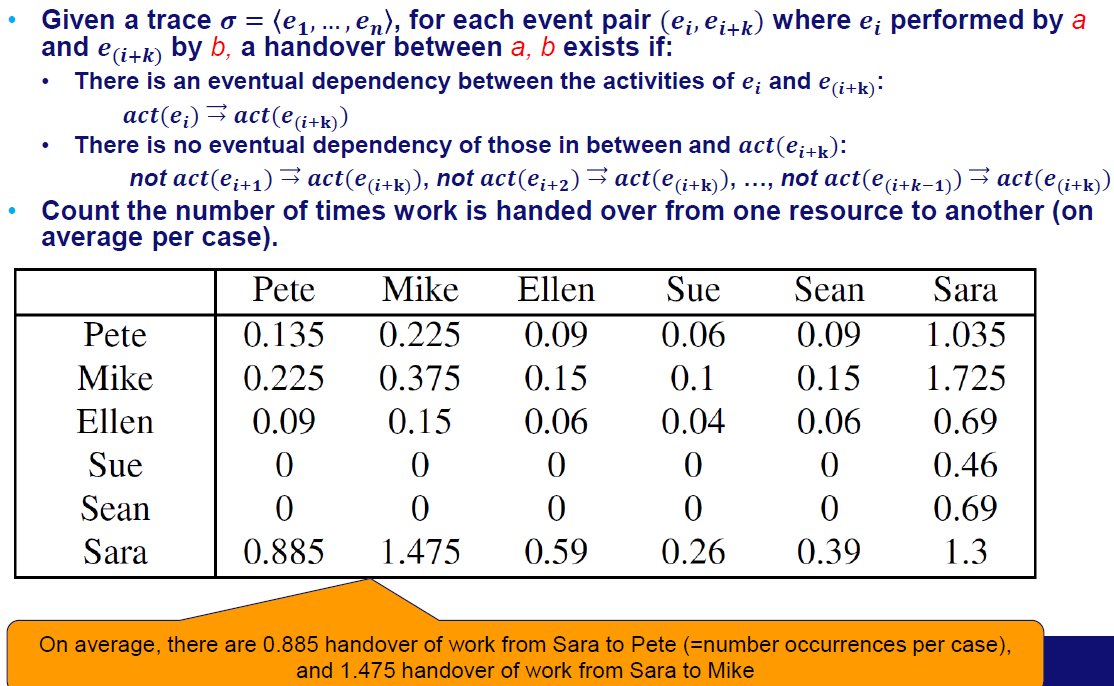
\includegraphics[width=0.7\textwidth]{capitolo 8/slide26.png}
\end{center}

\section{Data Perspective: Decision Mining}

The \textbf{data perspective} seeks to understand how choices are made between multiple paths in a process. For example:
\begin{itemize}
    \item Decision point: Choice between activities \(b\) and \(c\),
    \item Predictor variables: Resource, customer type, or monetary amount.
\end{itemize}

From the event log, patterns of decisions can be extracted. Probabilities of taking one path over another can be inferred, enabling the addition of \textbf{guards}, which specify conditions for decisions:
\[
\text{If Customer = Silver, take path \(b\); otherwise, take path \(c\)}.
\]
\begin{center}
    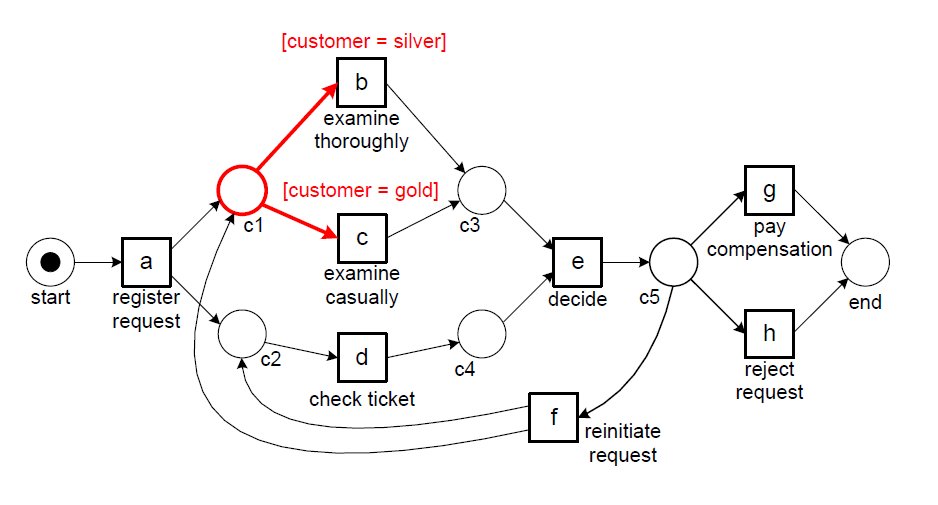
\includegraphics[width=0.7\textwidth]{capitolo 8/slide40.png}
\end{center}
We call the response variable when there is a choice, in this case between b and c. The predictor variables are attributes that are needed for the decision.

\section{Time Perspective}

The \textbf{time perspective} analyzes how long processes take:
\begin{itemize}
    \item Measure time between transitions,
    \item Identify bottlenecks where delays occur.
\end{itemize}

For example:
\begin{itemize}
    \item Long durations may indicate process blocks,
    \item Short durations suggest efficient execution.
\end{itemize}

\begin{center}
    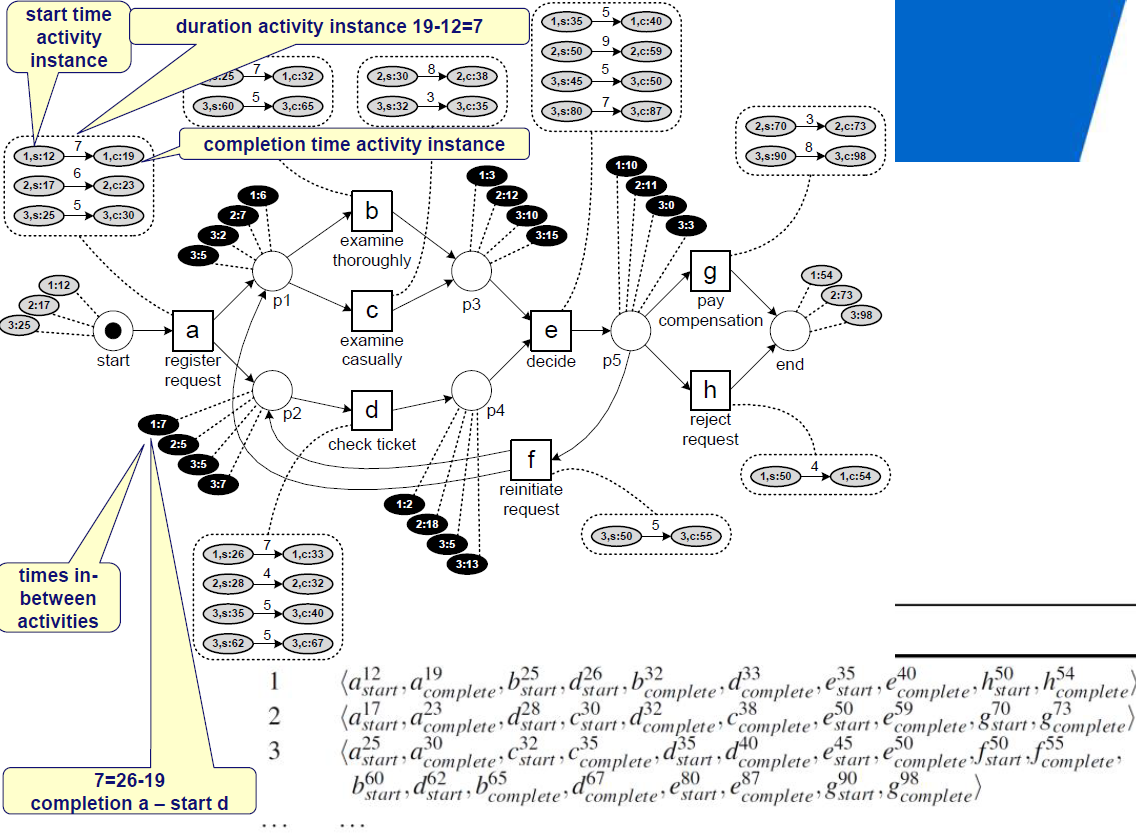
\includegraphics[width=0.7\textwidth]{capitolo 8/slide48.png}
    
\end{center}

\section{Alignments in Process Mining}

In real-world scenarios, traces may not perfectly fit the model due to:
\begin{itemize}
    \item Missing or incorrect data,
    \item Rare or exceptional cases.
\end{itemize}

\textbf{Alignments} fix traces by matching them to the "closest" path in the model, enabling:
\begin{itemize}
    \item Detection of deviations,
    \item Preservation of as much data as possible.
\end{itemize}

\section{Conclusion}

Exploring additional perspectives enriches our understanding of processes by incorporating aspects of organizational, decision, and time. This holistic approach enables more accurate and insightful process analysis, supporting better decision making and optimization.

\section{Convergence in Probability Theory}  
We aim to explore the meaning of convergence for sequences of random variables. Recall that a random variable, despite its name, can be viewed as a function. This allows us to draw parallels between convergence for sequences of functions and sequences of random variables.  

\subsection{Pointwise Convergence of Numbers and Functions}  
Consider a sequence of real numbers \(X_n\). We say that \(X_n\) converges to \(X\) as \(n \to \infty\) if, for any \(\epsilon > 0\):  
\[
\exists \, N \in \mathbb{N} \text{ such that } \forall n \geq N, \, |X_n - X| < \epsilon.
\]
This definition implies that for sufficiently large \(n\), all values of \(X_n\) fall within an \(\epsilon\)-neighborhood of \(X\). \newline
Similarly, for a sequence of functions \(f_n(x)\), we say \(f_n(x)\) converges pointwise to \(f(x)\) if:
\[
\lim_{n \to \infty} f_n(x) = f(x) \quad \forall x \in \text{Domain}(f).
\]
This is termed pointwise convergence. While widely used, mathematicians often prefer stronger notions such as uniform convergence due to its desirable properties, such as the preservation of continuity.  

\subsection{Almost Sure Convergence of Random Variables}  
Let \(\{X_n\}_{n=1}^\infty\) be a sequence of random variables defined on the same probability space \((\Omega, \mathcal{F}, \mathbb{P})\), and let \(X\) be another random variable. We say \(X_n\) converges to \(X\) \textbf{almost surely} (a.s.) as \(n \to \infty\) if:  
\[
\mathbb{P} \left( \omega \in \Omega : \lim_{n \to \infty} X_n(\omega) = X(\omega) \right) = 1.
\]
We write:
\[
X_n \xrightarrow{\text{a.s.}} X.
\]
This means that the sequence \(X_n(\omega)\) converges to \(X(\omega)\) for almost every \(\omega \in \Omega\), except possibly on a set of probability zero.  

\subsection{Convergence in Probability}  
Another notion of convergence for random variables is convergence in probability. Let \(\{X_n\}_{n=1}^\infty\) be a sequence of random variables and \(X\) another random variable on the same probability space. We say that \(X_n\) converges to \(X\) in probability, written as:
\[
X_n \xrightarrow{\mathbb{P}} X,
\]
if, for any \(\epsilon > 0\):
\[
\lim_{n \to \infty} \mathbb{P}(|X_n - X| \geq \epsilon) = 0.
\]
This definition implies that for large \(n\), the probability of \(X_n\) being farther than \(\epsilon\) from \(X\) becomes arbitrarily small.  

\subsubsection{Understanding the Probability Event}  
The event \(|X_n - X| \geq \epsilon\) can be expressed as:
\[
\{\omega \in \Omega : |X_n(\omega) - X(\omega)| \geq \epsilon\}.
\]
This is equivalent to:
\[
\{\omega \in \Omega : X_n(\omega) \not\in [X(\omega) - \epsilon, X(\omega) + \epsilon]\}.
\]
Thus, for convergence in probability, we require that the probability of \(X_n\) falling outside the \(\epsilon\)-neighborhood of \(X\) decreases to zero as \(n \to \infty\).  

\paragraph{Comparison of Convergence Types}  
\begin{itemize}  
    \item Almost Sure Convergence: Guarantees that \(X_n(\omega) \to X(\omega)\) for almost all \(\omega\). This is a strong form of convergence.  
    \item Convergence in Probability: Weaker than almost sure convergence. It ensures that the sequence of random variables is "close" to \(X\) with high probability, but this closeness may vary for different subsets of \(\Omega\) as \(n\) changes.  
\end{itemize}  

\subsection{Theorem: Convergence Almost Surely Implies Convergence in Probability}  
If \( X_n \to X \) almost surely as \( n \to \infty \), then:
\[
\mathbb{P} \left( \limsup_{n \to \infty} |X_n - X| \geq \epsilon \right) = 0 \quad \text{for all} \, \epsilon > 0.
\]
This means that if \( X_n \) converges to \( X \) almost surely, the probability that the distance between \( X_n \) and \( X \) is greater than any fixed \( \epsilon \) infinitely often is zero.

\subsubsection{Corollary: Sufficient Condition for Almost Sure Convergence}  
By the Borel-Cantelli Lemma, we know that if the sum:
\[
\sum_{n=1}^{\infty} \mathbb{P} \left( |X_n - X| \geq \epsilon \right) < \infty
\]
is finite, then \( X_n \to X \) almost surely. This provides a sufficient condition for almost sure convergence. If \(X_n \xrightarrow{\text{a.s.}} X\), then \(X_n \xrightarrow{\mathbb{P}} X\). However, the converse is not necessarily true. Convergence in probability does not imply almost sure convergence because the subset of \(\Omega\) where \(X_n\) does not converge to \(X\) may change with \(n\), even if the probability of such a subset becomes arbitrarily small. 

\section{Counterexample for Convergence in Probability but Not Almost Surely}

It is possible to construct a sequence of random variables \( \{X_n\}_{n=1}^\infty \) that converges to a random variable \( X \) in probability but does not converge almost surely to any random variable. This highlights that convergence in probability does not necessarily imply almost sure convergence.

\paragraph{Counterexample: A Constructive Approach}
Let us consider the sequence \( X_n \) defined as follows:
\begin{itemize}
    \item \( X_n \sim \text{Binomial}(1, p_n) \), where \( p_n \) varies depending on \( n \).
    \item We construct \( X_n \) using the unit interval \( \Omega = [0, 1] \) with the Lebesgue measure as the probability measure.
\end{itemize}

\paragraph{Construction of the Sequence:}
\begin{enumerate}
    \item Define \( X_1 \) such that:
    \[
    X_1(x) =
    \begin{cases}
    1 & \text{if } x \in [0, \frac{1}{2}), \\
    0 & \text{if } x \in [\frac{1}{2}, 1].
    \end{cases}
    \]
    Clearly, \( X_1 \sim \text{Binomial}(1, \frac{1}{2}) \).
    
    \item Define \( X_2 \) as:
    \[
    X_2(x) =
    \begin{cases}
    0 & \text{if } x \in [0, \frac{1}{2}), \\
    1 & \text{if } x \in [\frac{1}{2}, 1].
    \end{cases}
    \]
    Again, \( X_2 \sim \text{Binomial}(1, \frac{1}{2}) \), but note that \( X_1(x) \neq X_2(x) \) for all \( x \in [0, 1] \).

    \item Continue this construction, dividing the interval \([0, 1]\) into \( n \) equal parts for \( X_n \). Define \( X_n \) such that \( X_n(x) = 1 \) for one subinterval and \( 0 \) elsewhere. For instance:
    \[
    X_3(x) =
    \begin{cases}
    1 & \text{if } x \in [0, \frac{1}{3}), \\
    0 & \text{otherwise}.
    \end{cases}
    \]
    \item Similarly:
    \[
    X_4(x) =
    \begin{cases}
    1 & \text{if } x \in [\frac{1}{3}, \frac{2}{3}), \\
    0 & \text{otherwise}.
    \end{cases}
    \]
\end{enumerate}

\paragraph{Properties of the Construction:}
\begin{itemize}
    \item For any fixed \( x \in [0, 1] \), the sequence \( \{X_n(x)\} \) alternates between \( 0 \) and \( 1 \), depending on the subinterval to which \( x \) belongs.
    \item Each \( X_n \sim \text{Binomial}(1, \frac{1}{n}) \). As \( n \to \infty \), the probability \( p_n = \frac{1}{n} \) decreases, making \( X_n(x) \) increasingly likely to be \( 0 \).
\end{itemize}
We now show that \( X_n \to 0 \) in probability:
\[
\mathbb{P}(|X_n - 0| > \epsilon) = \mathbb{P}(X_n = 1) = p_n = \frac{1}{n}.
\]
As \( n \to \infty \), \( \frac{1}{n} \to 0 \). Therefore, \( X_n \to 0 \) in probability. \newline
For almost sure convergence, we consider any fixed \( x \in [0, 1] \). The sequence \( \{X_n(x)\} \) alternates between \( 0 \) and \( 1 \) infinitely often due to the construction. Thus:
\[
\limsup_{n \to \infty} X_n(x) = 1, \quad \liminf_{n \to \infty} X_n(x) = 0.
\]
Since the limits do not coincide, the sequence \( \{X_n(x)\} \) does not converge almost surely to any random variable. \newline
This counterexample demonstrates:
\begin{enumerate}
    \item Convergence in probability does not imply almost sure convergence.
    \item Almost sure convergence is a stronger form of convergence that requires the sequence to settle on a limit for almost every \( x \) in \( \Omega \).
\end{enumerate}
The distinction between convergence in probability and almost sure convergence is fundamental in understanding the Law of Large Numbers (LLN):
\begin{itemize}
    \item Weak LLN: Proves convergence in probability for the sample mean \( \bar{X}_n \).
    \item Strong LLN: Proves almost sure convergence for \( \bar{X}_n \).
\end{itemize}
These results will be explored in detail in subsequent sections.


\section{Convergence in $L^P$ Norm and Weak Convergence}

\subsection{Convergence in $L^P$ Norm}  
We now consider another type of convergence called convergence in \( L^p \)-norm. Recall that a random variable \( X \) belongs to \( L^1 \) (the space of square-integrable random variables) if and only if the expectation of \( X \) is finite:
\[
\mathbb{E}[|X|] < \infty.
\]
Similarly, \( X \in L^2 \) if and only if the expectation of the absolute value of \( X^2 \) is finite:
\[
\mathbb{E}[|X|^2] < \infty.
\]
For \( p = 3 \), \( X \in L^3 \) if and only if \( \mathbb{E}[|X|^3] < \infty \). In general, we define that \( X \in L^p \) for any \( p \geq 1 \) if and only if:
\[
\mathbb{E}[|X|^p] < \infty.
\]
This defines the space \( L^p \), which contains random variables whose absolute value raised to the power \( p \) has a finite expectation.

\subsubsection{Definition}  
Let \( \{X_n\}_{n=1}^\infty \) be a sequence of random variables and \( X \) another random variable, both defined on the same probability space. We say that \( X_n \) converges to \( X \) in \( L^p \)-norm as \( n \to \infty \) if:
\[
\lim_{n \to \infty} \mathbb{E}[|X_n - X|^p] = 0.
\]
This is the definition of convergence in \( L^p \)-norm. All the random variables in the sequence must belong to the same probability space and to the space \( L^p \) (i.e., their moments of order \( p \) must be finite).

\subsection{Weak Convergence (Convergence in Distribution)}  
The fourth type of convergence is called weak convergence, or convergence in distribution. Weak convergence is conceptually different from the previous types of convergence discussed. While the previous types required the random variables to be defined on the same probability space, weak convergence applies to random variables that may not share the same probability space. \newline
Let \( \{X_n\}_{n=1}^\infty \) be a sequence of random variables and \( X \) another random variable. We say that \( X_n \) converges to \( X \) in distribution, which is represented with \(X_n \xrightarrow{\mathcal{D}^w} X\), then \(X_n \xrightarrow{\mathbb{P}} X\) as \( n \to \infty \) if:
\[
F_{X_n}(x) \to F_X(x) \quad \text{for all } x \in \mathbb{R} \text{ where } F_X(x) \text{ is continuous}.
\]
Here, \( F_{X_n}(x) \) is the cumulative distribution function (CDF) of \( X_n \) and \( F_X(x) \) is the CDF of \( X \). The convergence happens at all points where \( F_X(x) \) is continuous. \newline
This type of convergence is also known as convergence in distribution, and it does not require the random variables to be defined on the same probability space. We simply require the convergence of their distribution functions.

\subsubsection{Further Results: Weak Convergence and Distribution Functions}

\begin{itemize}
    \item Weak convergence does not require the random variables to be defined on the same probability space. It only involves the convergence of their distribution functions.
    \item Convergence in distribution is typically used when analyzing large sample properties, such as the Central Limit Theorem (CLT), where we are interested in the behavior of the distribution rather than individual realizations of the random variables.
\end{itemize}


\section{The Weak Law of Large Numbers (WLLN)}
Let \( \{X_n\}_{n \geq 1} \) be a sequence of i.i.d. random variables, where "i.i.d." stands for independent and identically distributed. This means:
\begin{itemize}
    \item All random variables \( X_i \) share the same distribution (e.g., all are Binomial, Gaussian, or Exponential with the same parameter).
    \item The \( X_i \) are mutually independent.
\end{itemize}
Let \( \mu = \mathbb{E}[X_i] \), and assume that \( \mu \) is finite. This implies \( X_i \in L^1 \). Since all \( X_i \) share the same distribution, they have the same expectation \( \mu \). Additionally, assume that the variance \( \sigma^2 = \mathrm{Var}(X_i) \) is finite. For any \( \epsilon > 0 \), the following holds:
\[
\mathbb{P}(|\bar{X}_n - \mu| \geq \epsilon) \leq \frac{\sigma^2}{n \epsilon^2},
\]
where:
\[
\bar{X}_n = \frac{1}{n} \sum_{i=1}^n X_i
\]
is the sample mean of \( X_1, \dots, X_n \). \newline
This inequality implies that the probability of the sample mean deviating from the population mean \( \mu \) by more than \( \epsilon \) becomes arbitrarily small as \( n \to \infty \). Specifically, the right-hand side \( \frac{\sigma^2}{n \epsilon^2} \) approaches \( 0 \) as \( n \to \infty \). \newline
The sample mean \( \bar{X}_n \) converges to \( \mu \) in probability, denoted as:
\[
\bar{X}_n \xrightarrow{\mathbb{P}} \mu.
\]
This means that for any \( \epsilon > 0 \):
\[
\lim_{n \to \infty} \mathbb{P}(|\bar{X}_n - \mu| \geq \epsilon) = 0.
\]
In order to prove it we need to introduce the Markov Inequality and the Chebyshev Inequality.
\subsection{Markov Inequality}
The Markov inequality is a fundamental result in probability theory. It states that if \( Y \) is a non-negative random variable, and \( \delta > 0 \) is any positive constant, then:
\[
\mathbb{P}(Y \geq \delta) \leq \frac{\mathbb{E}[Y]}{\delta}.
\]

\paragraph{Proof:}  
For any \( Y \geq 0 \), we can write:
\[
Y \geq \delta \cdot \mathbb{I}(Y \geq \delta),
\]
where \( \mathbb{I}(Y \geq \delta) \) is the indicator function of the event \( Y \geq \delta \). The inequality holds because:
\begin{itemize}
    \item If \( Y \geq \delta \), then \( \mathbb{I}(Y \geq \delta) = 1 \), and \( Y \geq \delta \) is trivially true.
    \item If \( Y < \delta \), then \( \mathbb{I}(Y \geq \delta) = 0 \), and \( Y \geq 0 \) holds because \( Y \) is non-negative.
\end{itemize}
Taking expectations on both sides:
\[
\mathbb{E}[Y] \geq \delta \cdot \mathbb{E}[\mathbb{I}(Y \geq \delta)].
\]
Since the expectation of an indicator function corresponds to the probability of the event it represents:
\[
\mathbb{E}[\mathbb{I}(Y \geq \delta)] = \mathbb{P}(Y \geq \delta).
\]
Thus:
\[
\mathbb{E}[Y] \geq \delta \cdot \mathbb{P}(Y \geq \delta).
\]
Dividing both sides by \( \delta \) gives:
\[
\mathbb{P}(Y \geq \delta) \leq \frac{\mathbb{E}[Y]}{\delta}.
\]

\subsection{Chebyshev Inequality}
The Chebyshev inequality is a direct consequence of the Markov inequality. It provides a bound on the probability that a random variable deviates from its mean by a certain amount.

\paragraph{Theorem:}
Let \( X \in L^2 \), meaning \( \mathbb{E}[X^2] < \infty \). Then, for any \( \epsilon > 0 \):
\[
\mathbb{P}(|X - \mu| \geq \epsilon) \leq \frac{\mathrm{Var}(X)}{\epsilon^2},
\]
where \( \mu = \mathbb{E}[X] \) and \( \mathrm{Var}(X) = \mathbb{E}[(X - \mu)^2] \). \newline
Define \( Y = (X - \mu)^2 \), which is a non-negative random variable. Then:
\[
\mathbb{P}(|X - \mu| \geq \epsilon) = \mathbb{P}((X - \mu)^2 \geq \epsilon^2).
\]
Applying the Markov inequality to \( Y \) with \( \delta = \epsilon^2 \), we get:
\[
\mathbb{P}((X - \mu)^2 \geq \epsilon^2) \leq \frac{\mathbb{E}[(X - \mu)^2]}{\epsilon^2}.
\]
By definition of variance, \( \mathbb{E}[(X - \mu)^2] = \mathrm{Var}(X) \). Thus:
\[
\mathbb{P}(|X - \mu| \geq \epsilon) \leq \frac{\mathrm{Var}(X)}{\epsilon^2}.
\]

\subsection{Application to the Weak Law of Large Numbers (WLLN)}

Consider the sequence \( \{X_i\}_{i=1}^n \), where \( X_i \) are independent and identically distributed (i.i.d.) random variables with mean \( \mu \) and variance \( \sigma^2 \). Define the sample mean:
\[
\bar{X}_n = \frac{1}{n} \sum_{i=1}^n X_i.
\]

\paragraph{Key Properties of \( \bar{X}_n \):}
\begin{enumerate}
    \item Expectation:
    \[
    \mathbb{E}[\bar{X}_n] = \frac{1}{n} \sum_{i=1}^n \mathbb{E}[X_i] = \mu.
    \]
    \item Variance:
    \[
    \mathrm{Var}(\bar{X}_n) = \mathrm{Var}\left(\frac{1}{n} \sum_{i=1}^n X_i \right) = \frac{1}{n^2} \sum_{i=1}^n \mathrm{Var}(X_i).
    \]
    Since \( X_i \) are i.i.d., \( \mathrm{Var}(X_i) = \sigma^2 \), so:
    \[
    \mathrm{Var}(\bar{X}_n) = \frac{1}{n^2} \cdot n \cdot \sigma^2 = \frac{\sigma^2}{n}.
    \]
\end{enumerate}

\paragraph{Weak Law of Large Numbers (WLLN):}
Using the Chebyshev inequality:
\[
\mathbb{P}(|\bar{X}_n - \mu| \geq \epsilon) \leq \frac{\mathrm{Var}(\bar{X}_n)}{\epsilon^2} = \frac{\sigma^2}{n \epsilon^2}.
\]
As \( n \to \infty \), \( \frac{\sigma^2}{n \epsilon^2} \to 0 \). Therefore:
\[
\bar{X}_n \xrightarrow{\mathbb{P}} \mu,
\]
i.e., \( \bar{X}_n \) converges in probability to \( \mu \). This inequality shows that the probability of the sample mean deviating from the true mean \( \mu \) diminishes as \( n \to \infty \). Specifically, it converges to \( 0 \) at a rate proportional to \( \frac{1}{n} \).

\section{Chernoff Bounds: Derivation and Application}
While the WLLN guarantees convergence in probability, it is often beneficial to analyze the rate of convergence. The Chebyshev bound suggests a convergence rate of \( \mathcal{O}(1/n) \), which, while useful, is not particularly rapid. To refine the bounds on probabilities of deviations in the sample mean, we proceed with the analysis of the following inequality for \( \bar{X}_n = \frac{1}{n} \sum_{i=1}^n X_i \). We get that the upper tail estimate is:
\[
\mathbb{P}(\bar{X}_n \geq \mu + \epsilon) \leq \exp(-n G(t)),
\]
where \( G(t) \) is a carefully defined function derived from the moment-generating function of \( X_i \). 

\subsubsection{Step 1: Rewriting the Probability as an Exponential}
The initial probability can be expressed as:
\[
\mathbb{P}(\bar{X}_n \geq \mu + \epsilon) = \mathbb{P}\left(\sum_{i=1}^n X_i \geq n(\mu + \epsilon)\right).
\]
Exponentiating both sides using the monotonicity of the exponential function, with $t>0$, gives:
\[
\mathbb{P}\left(\sum_{i=1}^n X_i \geq n(\mu + \epsilon)\right) = \mathbb{P}\left(e^{t \sum_{i=1}^n X_i} \geq e^{t n (\mu + \epsilon)}\right).
\]
Using Markov's inequality, we obtain:
\[
\mathbb{P}\left(e^{t \sum_{i=1}^n X_i} \geq e^{t n (\mu + \epsilon)}\right) \leq \frac{\mathbb{E}[e^{t \sum_{i=1}^n X_i}]}{e^{t n (\mu + \epsilon)}}.
\]

\subsubsection{Step 2: Leveraging Independence and Moment-Generating Functions}
Exploiting the independence of the \( X_i \), the expectation in the numerator becomes:
\[
\mathbb{E}\left[e^{t \sum_{i=1}^n X_i}\right] = \prod_{i=1}^n \mathbb{E}\left[e^{t X_i}\right] = \left(\mathbb{E}[e^{t X_1}]\right)^n = \left(M(t)\right)^n,
\]
where \( M(t) = \mathbb{E}[e^{t X_1}] \) is the moment-generating function of \( X_1 \). Substituting this into the inequality yields:
\[
\mathbb{P}(\bar{X}_n \geq \mu + \epsilon) \leq \frac{\left(M(t)\right)^n}{e^{t n (\mu + \epsilon)}}.
\]

\subsubsection{Step 3: Simplifying the Expression}
Rewriting the ratio as a single exponential:
\[
\frac{\left(M(t)\right)^n}{e^{t n (\mu + \epsilon)}} = \exp\left(n \ln M(t) - t n (\mu + \epsilon)\right).
\]
Define \( G(t) \) as:
\[
G(t) = t (\mu + \epsilon) - \ln M(t).
\]
Thus:
\[
\mathbb{P}(\bar{X}_n \geq \mu + \epsilon) \leq \exp\left(-n G(t)\right).
\]

\subsubsection{Step 4: Optimizing \( G(t) \)}
The utility of this bound depends on the behavior of \( G(t) \). Specifically:
\begin{itemize}
    \item If \( G(t) > 0 \), the bound converges to zero exponentially as \( n \to \infty \).
    \item To tighten the bound, we maximize \( G(t) \) for \( t \geq 0 \). Let \( t^* \) be the maximizer, such that:
    \[
    G(t^*) = \max_{t \geq 0} G(t).
    \]
    \item Substituting \( t^* \) into the bound provides the sharpest estimate:
    \[
    \mathbb{P}(\bar{X}_n \geq \mu + \epsilon) \leq \exp\left(-n G(t^*)\right).
    \]
\end{itemize}

\subsubsection{Step 5: Analysis of \( G(t) \), with $t>0$}
The function \( G(t) \) is given by:
\[
G(t) = t \cdot (\mu + \epsilon) - \ln M(t).
\]
\begin{itemize}
    \item At \( t = 0 \), \( G(0) = 0 \), since \( \ln M(0) = \ln 1 = 0 \).
    \item The derivative is:
    \[
    G'(t) = (\mu + \epsilon) - \frac{M'(t)}{M(t)}.
    \]
    At \( t = 0 \):
    \[
    G'(0) = (\mu + \epsilon) - \mu = \epsilon > 0.
    \]
    Since \( G'(0) > 0 \), \( G(t) \) increases for small \( t > 0 \). This guarantees the existence of a \( t^* > 0 \) where \( G(t^*) > 0 \).
\end{itemize}

\subsubsection{Step 6: Extending to the Lower Tail}
A similar argument applies for the lower tail:
\[
\mathbb{P}(\bar{X}_n \leq \mu - \epsilon) \leq \exp\left(-n H(t)\right),
\]
where \( H(t) \) is defined as:
\[
H(t) = -t (\mu - \epsilon) - \ln M(-t).
\]
\begin{itemize}
    \item \( H(0) = 0 \).
    \item The derivative:
    \[
    H'(t) = -(\mu - \epsilon) + \frac{M'(-t)}{M(-t)}.
    \]
    At \( t = 0 \), \( H'(0) = \epsilon > 0 \), ensuring \( H(t) > 0 \) for small \( t > 0 \).
\end{itemize}

\subsubsection{Conclusion}
Combining the upper and lower tail bounds:
\[
\mathbb{P}(|\bar{X}_n - \mu| \geq \epsilon) \leq 2 \exp\left(-n G(t^*)\right),
\]
where \( G(t^*) \) is the maximum of \( G(t) \) for \( t \geq 0 \). This result showcases the exponential decay of probabilities, significantly improving over earlier polynomial bounds.

\section{Chernoff Bounds: Extension to the Lower Tail and Example with Gaussian Random Variables}

\subsection{Example 1: Standard Normal Variables}
The Gaussian random variable case provides an excellent starting point to understand Chernoff bounds. Let us consider independent copies of a standard normal random variable \( X_i \sim \mathcal{N}(0, 1) \).
\begin{itemize}
    \item For the standard normal, the expectation \( \mu = 0 \) and the moment-generating function is:
    \[
    M(t) = \mathbb{E}[e^{t X}] = e^{t^2 / 2}, \quad t \in \mathbb{R}.
    \]
    \item The upper-tail probability is bounded as:
    \[
    \mathbb{P}(\bar{X}_n \geq \mu + \epsilon) \leq \exp\left(-n G(t^*)\right),
    \]
    where \( G(t) = t (\mu + \epsilon) - \ln M(t) \).
\end{itemize}
Substituting \( \mu = 0 \) and \( \ln M(t) = t^2 / 2 \), the function \( G(t) \) becomes:
\[
G(t) = t \epsilon - \frac{t^2}{2}.
\]

\subsubsection{Analysis of \( G(t) \)}
\begin{itemize}
    \item The function \( G(t) = t \epsilon - \frac{t^2}{2} \) is quadratic in \( t \). Its maximum occurs at \( t = \epsilon \), which is the vertex of the parabola.
    \item At \( t = \epsilon \):
    \[
    G(t^*) = G(\epsilon) = \epsilon^2 / 2.
    \]
\end{itemize}
Thus, the Chernoff bound for the Gaussian case becomes:
\[
\mathbb{P}(\bar{X}_n \geq \mu + \epsilon) = \mathbb{P}(\bar{X}_n \geq \epsilon) \leq \exp\left(-\frac{n \epsilon^2}{2}\right).
\]

\subsubsection{Remark on the Gaussian Case}
For Gaussian random variables, we can derive even tighter bounds using properties specific to the normal distribution. By leveraging additional tools, the probability of a standard normal exceeding a threshold \( x \) satisfies:
\[
\mathbb{P}(X \geq x) \leq \frac{1}{x \sqrt{2\pi}} e^{-x^2 / 2}, \quad x \geq 0.
\]
This result improves upon the Chernoff bound by including a prefactor \( 1/x \), which accelerates convergence to zero.

\subsubsection{Generalization to Other Distributions}
The Gaussian case serves as a benchmark. For more general distributions, we aim to derive bounds that mimic the Gaussian behavior:
\[
\mathbb{P}(\bar{X}_n \geq \mu + \epsilon) \leq \exp\left(-n f(\epsilon)\right),
\]
where \( f(\epsilon) \) often involves \( \epsilon^2 \) or other polynomial dependencies on \( \epsilon \). \newline
For standard normal variables, we achieve sharper results using their specific properties. In the general setting, Chernoff bounds provide a robust framework for analyzing tail probabilities. The next step is to explore other "easy cases" and extend the bounds to more complex distributions.

\subsection{Example 2: Transformation of Standard Normal Variables}

Let us consider a family of independent standard normal random variables \( Z_1, Z_2, \ldots, Z_n \), where \( Z_i \sim \mathcal{N}(0, 1) \). For each \( i = 1, 2, \ldots, n \), we define a transformation of \( Z_i \) as:
\[
X_i = Z_i^2.
\]
These random variables \( X_i \) are said to follow a chi-square distribution with one degree of freedom:
\[
X_i \sim \chi^2(1).
\]
This distribution is also equivalent to a Gamma distribution:
\[
X_i \sim \Gamma\left(\frac{1}{2}, 1\right).
\]
The chi-square distribution arises naturally in statistics, especially in hypothesis testing and estimation.

\subsubsection{Moment-Generating Function of \( X_i \)}
To apply Chernoff bounds, we need the expectation and moment-generating function (MGF) of \( X_i \):
\begin{itemize}
    \item The expectation is:
    \[
    \mathbb{E}[X_i] = \mathbb{E}[Z_i^2] = \text{Var}(Z_i) = 1.
    \]
    \item The moment-generating function is:
    \[
    M_X(t) = \mathbb{E}[e^{t X_i}] = \mathbb{E}[e^{t Z_i^2}].
    \]
\end{itemize}
To compute \( M_X(t) \), we integrate over the density of the standard normal random variable:
\[
M_X(t) = \int_{-\infty}^{\infty} e^{t z^2} \cdot \frac{1}{\sqrt{2\pi}} e^{-z^2 / 2} \, dz = \frac{1}{\sqrt{2\pi}} \int_{-\infty}^\infty e^{-(1 - 2t)z^2 / 2} \, dz.
\]

\subsubsection{Evaluation of the Integral}

By completing the square and substituting \( s = \sqrt{1 - 2t} \cdot z \), we simplify the integral:
\[
M_X(t) = \frac{1}{\sqrt{2\pi}} \int_{-\infty}^\infty \frac{1}{\sqrt{1 - 2t}} e^{-s^2 / 2} \, ds.
\]
Since the integral of the standard normal density over \( s \) is 1, we obtain:
\[
M_X(t) =
\begin{cases}
\frac{1}{\sqrt{1 - 2t}}, & t < \frac{1}{2}, \\
\infty, & t \geq \frac{1}{2}.
\end{cases}
\]
The moment-generating function is finite for \( t < 1/2 \), which is sufficient to apply Chernoff bounds.

\subsubsection{Chernoff Bound for the Upper Tail}

The upper-tail probability is given by:
\[
\mathbb{P}\left(\bar{X}_n \geq \mu + \epsilon\right) \leq e^{-n G(t)},
\]
where \( G(t) = t (\mu + \epsilon) - \ln M_X(t) \). Substituting \( \mu = 1 \) and \( \ln M_X(t) = -\frac{1}{2} \ln(1 - 2t) \), we have:
\[
G(t) = t (1 + \epsilon) + \frac{1}{2} \ln(1 - 2t).
\]

\subsubsection{Maximizing \( G(t) \)}

To find the best bound, we maximize \( G(t) \) over \( t \in [0, 1/2) \). The derivative of \( G(t) \) is:
\[
G'(t) = (1 + \epsilon) - \frac{1}{1 - 2t}.
\]
Setting \( G'(t) = 0 \), we solve:
\[
(1 + \epsilon) = \frac{1}{1 - 2t}.
\]
Rearranging gives:
\[
1 - 2t = \frac{1}{1 + \epsilon}, \quad 2t = 1 - \frac{1}{1 + \epsilon} = \frac{\epsilon}{1 + \epsilon}, \quad t = \frac{\epsilon}{2(1 + \epsilon)}.
\]

\subsubsection{Optimal Value of \( G(t) \)}

Substituting \( t^* = \frac{\epsilon}{2(1 + \epsilon)} \) into \( G(t) \), we find:
\[
G(t^*) = t^* (1 + \epsilon) + \frac{1}{2} \ln\left(1 - 2t^*\right).
\]
Using \( 1 - 2t^* = \frac{1}{1 + \epsilon} \), this simplifies to:
\[
G(t^*) = \frac{\epsilon}{2} - \frac{1}{2} \ln(1 + \epsilon).
\]
Thus, the Chernoff bound becomes:
\[
\mathbb{P}\left(\bar{X}_n \geq 1 + \epsilon\right) \leq \exp\left(-n \left[\frac{\epsilon}{2} - \frac{1}{2} \ln(1 + \epsilon)\right]\right).
\]

\subsubsection{Approximation of \( \ln(1 + \epsilon) \)}
To simplify the bound, we approximate \( \ln(1 + \epsilon) \) for small \( \epsilon > 0 \). Specifically, we want to show:
\[
\ln(1 + \epsilon) \leq \epsilon - \frac{\epsilon^2}{2(1 + \epsilon)}.
\]

Define:
\[
A(\epsilon) = \ln(1 + \epsilon), \quad B(\epsilon) = \epsilon - \frac{\epsilon^2}{2(1 + \epsilon)}.
\]
We aim to prove \( A(\epsilon) \leq B(\epsilon) \) for small \( \epsilon \geq 0 \).

\paragraph{Step 1: Initial Values.}
At \( \epsilon = 0 \):
\[
A(0) = \ln(1) = 0, \quad B(0) = 0.
\]
Thus, \( A(0) = B(0) \).

\paragraph{Step 2: Derivatives.}
The derivatives of \( A(\epsilon) \) and \( B(\epsilon) \) are:
\[
A'(\epsilon) = \frac{1}{1 + \epsilon}, \quad
B'(\epsilon) = 1 - \frac{\epsilon(2 + \epsilon)}{2(1 + \epsilon)^2}.
\]

If \( A'(\epsilon) \leq B'(\epsilon) \) for small \( \epsilon \geq 0 \), then \( A(\epsilon) \leq B(\epsilon) \).

\paragraph{Step 3: Simplifying the Inequality.}
We compare \( A'(\epsilon) \) and \( B'(\epsilon) \). The inequality \( \frac{1}{1 + \epsilon} \leq 1 - \frac{\epsilon(2 + \epsilon)}{2(1 + \epsilon)^2} \) reduces to:
\[
2(1 + \epsilon)^2 \leq 2 + 2\epsilon + \epsilon^2.
\]
Expanding both sides confirms this inequality holds for small \( \epsilon \geq 0 \).

\subsubsection{Final Bound}

Using the approximation \( \ln(1 + \epsilon) \leq \epsilon - \frac{\epsilon^2}{2(1 + \epsilon)} \), the function \( G(t^*) \) becomes:
\[
G(t^*) \geq \frac{\epsilon^2}{4(1 + \epsilon)}.
\]
Thus, the upper tail estimate is:
\[
\mathbb{P}\left(\bar{X}_n \geq 1 + \epsilon\right) \leq \exp\left(-n \frac{\epsilon^2}{4(1 + \epsilon)}\right).
\]
This bound provides an exponential decay rate for the probability as \( n \to \infty \).

\subsubsection{Lower Tail Estimate Using Chernoff Bound}

To complement the upper tail estimate, we now focus on the *lower tail* bound. Specifically, we aim to estimate:
\[
\mathbb{P}\left(\bar{X}_n \leq \mu - \epsilon\right),
\]
where \( \bar{X}_n \) is the sample mean, \(\mu\) is the mean of the distribution of \(X_i\), and \(\epsilon > 0\). Using the Chernoff technique, this probability is bounded as follows:
\[
\mathbb{P}\left(\bar{X}_n \leq \mu - \epsilon\right) \leq \exp\left(-n H(t)\right),
\]
where the function \( H(t) \) is defined as:
\[
H(t) = -t (\mu - \epsilon) - \ln M_X(-t).
\]

\paragraph{Definition of \(H(t)\):}
For the case where \(X_i = Z_i^2\), with \(Z_i \sim \mathcal{N}(0, 1)\), we know that:
\[
M_X(t) = \begin{cases}
\frac{1}{\sqrt{1 - 2t}}, & \text{if } t < \frac{1}{2}, \\
\infty, & \text{if } t \geq \frac{1}{2}.
\end{cases}
\]
Thus:
\[
M_X(-t) = \frac{1}{\sqrt{1 + 2t}} \quad \text{for } t > 0.
\]
Substituting into \(H(t)\):
\[
H(t) = -t (\mu - \epsilon) + \frac{1}{2} \ln(1 + 2t).
\]
For \( t = 0 \), \( H(0) = 0 \), ensuring \(H(t) \geq 0\) for small values of \(t\).

\paragraph{Optimization of \(H(t)\):}
To find the optimal value of \(t\), we compute the derivative \(H'(t)\) and set it to zero:
\[
H'(t) = -(\mu - \epsilon) + \frac{1}{2} \cdot \frac{2}{1 + 2t}.
\]
Simplifying:
\[
H'(t) = -(\mu - \epsilon) + \frac{1}{1 + 2t}.
\]
Setting \(H'(t) = 0\):
\[
\frac{1}{1 + 2t} = \mu - \epsilon,
\]
which implies:
\[
1 + 2t = \frac{1}{\mu - \epsilon}.
\]
Thus:
\[
t^* = \frac{\frac{1}{\mu - \epsilon} - 1}{2} = \frac{\epsilon}{2(\mu - \epsilon)}.
\]

\paragraph{Evaluation of \(H(t^*)\):}
Substituting \(t^*\) back into \(H(t)\):
\[
H(t^*) = -t^*(\mu - \epsilon) + \frac{1}{2} \ln(1 + 2t^*).
\]
Using \(1 + 2t^* = \frac{1}{\mu - \epsilon}\), we find:
\[
H(t^*) = -\frac{\epsilon}{2(\mu - \epsilon)}(\mu - \epsilon) + \frac{1}{2} \ln\left(\frac{1}{\mu - \epsilon}\right).
\]
Simplifying:
\[
H(t^*) = -\frac{\epsilon}{2} + \frac{1}{2} \ln\left(\frac{1}{\mu - \epsilon}\right).
\]
For the case where \(\mu = 1\), the above reduces to:
\[
H(t^*) = -\frac{\epsilon}{2} + \frac{1}{2} \ln\left(\frac{1}{1 - \epsilon}\right).
\]

\paragraph{
Approximation for Logarithmic Term:}
To simplify further, we use the inequality:
\[
\l(1 - \epsilon) \leq -\epsilon - \frac{\epsilon^2}{2}.
\]
Thus:
\[
-\frac{\epsilon}{2} + \frac{1}{2} \ln\left(\frac{1}{1 - \epsilon}\right) \leq -\frac{\epsilon}{2} + \frac{1}{2}(-\epsilon - \frac{\epsilon^2}{2}) = -\frac{\epsilon^2}{4}.
\]

\paragraph{Final Lower Tail Bound:}
This yields the lower tail estimate:
\[
\mathbb{P}\left(\bar{X}_n \leq \mu - \epsilon\right) \leq \exp\left(-n \frac{\epsilon^2}{4}\right).
\]

\subsubsection{Summary of Chernoff Bounds}
Combining the upper and lower tail estimates:
\[
\mathbb{P}(|\bar{X}_n - \mu| \geq \epsilon) \leq 2 \exp\left(-n \frac{\epsilon^2}{8}\right).
\]
This provides a complete characterization of the deviation of the sample mean from the true mean for the squared normal random variables under the Chernoff bound framework.

\subsection{Advanced Probability Estimates for Normal and Binomial Distributions}

\paragraph{Probability Bounds for Normal Distributions.}
For a standard normal random variable \( X \), the probability that the sample mean \( \bar{X}_n \) deviates significantly from the mean can be tightly bounded. Specifically, we showed:
\[
\mathbb{P}(\bar{X}_n \geq \mu + \epsilon) \leq e^{-n\epsilon^2 / 2}.
\]
This result is particularly significant for its exponential decay rate, which implies rapid convergence of \( \bar{X}_n \) to the true mean \( \mu \). The probability of error decreases exponentially with \( n \), allowing us to achieve desired confidence levels with moderate sample sizes. \newline
For practical applications, if a specific small probability of error, say less than \( 0.01 \), is required, this inequality provides the necessary sample size \( n \). This reduces both computational and data collection costs while ensuring statistical accuracy.

\paragraph{Sharper Bounds Using the Density of Standard Normal Variables.}
The probability \( \mathbb{P}(X \geq x) \) for \( X \sim N(0, 1) \) can also be estimated directly using its probability density function (PDF). Recall that the PDF is given by:
\[
f_X(x) = \frac{1}{\sqrt{2\pi}} e^{-x^2 / 2}.
\]
To refine the estimate, we applied a differential equation associated with the density function:
\[
x f_X(x) = -f'_X(x).
\]
Using this property, we derived:
\[
\mathbb{P}(X \geq x) \leq \frac{1}{x} f_X(x),
\]
where \( x > 0 \). This estimate is particularly useful for tail probabilities in Gaussian distributions, as it leverages the exponential decay of \( f_X(x) \).

\paragraph{Application to Sample Means.}
For a sample mean \( \bar{X}_n \) of \( n \) independent \( N(0, 1) \) random variables, we observed that:
\[
\mathbb{P}(\bar{X}_n \geq \epsilon) = \mathbb{P}\left(\sqrt{n} \bar{X}_n \geq \sqrt{n} \epsilon\right),
\]
where \( \sqrt{n} \bar{X}_n \sim N(0, 1) \). Applying the sharper bound, we obtained:
\[
\mathbb{P}(\bar{X}_n \geq \epsilon) \leq \frac{1}{\epsilon \sqrt{n}} \frac{1}{\sqrt{2\pi}} e^{-n\epsilon^2 / 2}.
\]
This result demonstrates the added precision of including a multiplicative factor of \( 1 / \sqrt{n} \), further tightening the probability bounds.

\paragraph{Upper Tail Estimates for Binomial Distributions.}
For a sequence of \( n \) i.i.d. Bernoulli random variables \( X_i \sim \text{Bernoulli}(p) \), the moment-generating function (MGF) plays a critical role in deriving bounds:
\[
M(t) = p e^t + (1 - p).
\]
Using this MGF, the upper tail probability for the sample mean \( \bar{X}_n \) exceeding \( p + \delta \) can be bounded by:
\[
\mathbb{P}(\bar{X}_n \geq p + \delta) \leq e^{-n p \delta^2 / (2 + \delta)}.
\]
For small values of \( \delta \), this reduces to the simpler form:
\[
\mathbb{P}(\bar{X}_n \geq p + \delta) \leq e^{-n p \delta^2 / 2},
\]
providing a practical estimate with fewer computational demands.


\section{Chernoff Bounds for Discrete Random Variables}

We now turn our attention to the application of Chernoff bounds in the context of discrete random variables. Specifically, we analyze the scenario of independent and identically distributed (i.i.d.) random variables taking discrete values. 

\subsection{Bernoulli Random Variables}
Consider \( X_1, X_2, \dots, X_n \), where each \( X_i \) is a Bernoulli random variable with parameter \( p \). That is:
\[
\mathbb{P}(X_i = 1) = p, \quad \mathbb{P}(X_i = 0) = 1 - p.
\]
The expectation of \( X_i \) is:
\[
\mu = \mathbb{E}[X_i] = p.
\]
The moment-generating function (MGF) of \( X_i \) is given by:
\[
M_X(t) = \mathbb{E}\left[e^{t X_i}\right] = p e^t + (1 - p).
\]

\paragraph{Upper Tail Estimate}
We seek to bound:
\[
\mathbb{P}(\bar{X}_n \geq \mu + \epsilon),
\]
where \( \bar{X}_n = \frac{1}{n} \sum_{i=1}^n X_i \) is the sample mean. Using the Chernoff technique:
\[
\mathbb{P}(\bar{X}_n \geq \mu + \epsilon) \leq \exp\left(-n G(t)\right),
\]
where:
\[
G(t) = t (\mu + \epsilon) - \ln M_X(t).
\]
Substituting \( \mu = p \), the function \( G(t) \) becomes:
\[
G(t) = t (p + \epsilon) - \ln\left[p e^t + (1 - p)\right].
\]

\paragraph{Optimization of \( G(t) \)}
To find the optimal bound, we maximize \( G(t) \) by solving:
\[
G'(t) = (p + \epsilon) - \frac{p e^t}{p e^t + (1 - p)} = 0.
\]
Simplifying:
\[
p e^t + (1 - p) = \frac{p e^t}{p + \epsilon},
\]
which leads to:
\[
e^t = \frac{(p + \epsilon)(1 - p)}{p (1 - p - \epsilon)}.
\]
Taking the natural logarithm gives the optimal \( t^* \):
\[
t^* = \ln\left(\frac{(p + \epsilon)(1 - p)}{p (1 - p - \epsilon)}\right).
\]

\paragraph{Final Bound}
Substituting \( t^* \) into \( G(t) \):
\[
G(t^*) = t^* (p + \epsilon) - \ln\left[p e^{t^*} + (1 - p)\right].
\]
While this expression can be evaluated numerically, it is generally unwieldy. To simplify, we use the inequality:
\[
\l(1 + x) \leq x.
\]
This allows us to approximate \( G(t) \) and derive a looser but more interpretable bound. Ultimately, we find:
\[
\mathbb{P}(\bar{X}_n \geq \mu + \epsilon) \leq \exp\left(-n \frac{\epsilon^2}{2p}\right),
\]
valid for \( \epsilon \leq p \).

\paragraph{Remarks on Tightening the Bound}
While the Chernoff bound provides a general framework, additional tricks or properties specific to the random variable can yield sharper estimates. For instance, for Gaussian random variables, specific properties of the normal distribution allow the derivation of more refined tail bounds. Similarly, for Bernoulli variables, leveraging the binomial structure may produce tighter results, though these can involve more intricate computations.

\paragraph{Summary}
Chernoff bounds serve as a versatile tool for bounding probabilities of rare events, particularly for sums of i.i.d. random variables. While exact computation can be challenging, the framework provides a principled approach to understanding deviations in both discrete and continuous cases.

\section{Central Limit Theorem: Upper Tail Estimate and General Proof}

\paragraph{Upper Tail Estimate.}
The probability that the sample mean deviates above its expected value by at least a fraction \(\delta\) of the true mean can be bounded as follows:
\[
\mathbb{P}(\bar{X}_n \geq (1 + \delta) \mu) \leq \exp\left(-n \mu \frac{\delta^2}{2 + \delta}\right),
\]
where we denote \(\epsilon = \delta \mu\) for notational simplicity. \newline
This result is a direct consequence of applying Chernoff bounds, where the quadratic term \(\delta^2\) dominates the behavior of the bound. For small \(\delta\), we observe that the denominator \(2 + \delta\) can be approximated by a constant, simplifying the estimate further. This makes Chernoff bounds particularly powerful for analyzing deviations in sums of random variables.

\paragraph{Introduction to the Central Limit Theorem.}
The Central Limit Theorem (CLT) forms the foundation of statistical inference. Consider a sequence of independent and identically distributed (i.i.d.) random variables \((X_n)_{n \in \mathbb{N}}\), each with finite mean \(\mu = \mathbb{E}[X_i]\) and variance \(\sigma^2 = \mathrm{Var}(X_i) > 0\). Define the standardized variable:
\[
Z_n = \frac{\sqrt{n} (\bar{X}_n - \mu)}{\sigma},
\]
where \(\bar{X}_n = \frac{1}{n} \sum_{i=1}^n X_i\) is the sample mean. Substituting \(\bar{X}_n\) into \(Z_n\), we rewrite:
\[
Z_n = \frac{1}{\sqrt{n} \sigma} \sum_{i=1}^n (X_i - \mu).
\]
The Central Limit Theorem asserts that:
\[
Z_n \xrightarrow{D} \mathcal{N}(0, 1),
\]
where \(\mathcal{N}(0, 1)\) denotes the standard normal distribution. This remarkable result holds regardless of the underlying distribution of \(X_i\), provided \(\mathbb{E}[X_i^2] < \infty\).

\paragraph{Intuition Behind the CLT.}
\begin{enumerate}
    \item Law of Large Numbers: The sample mean \(\bar{X}_n\) converges in probability (and almost surely) to the true mean \(\mu\):
   \[
   \bar{X}_n \xrightarrow{\mathbb{P}} \mu.
   \]
   This implies that the sum of \(n\) independent observations grows linearly with \(n\), but the mean stabilizes.
   \item Variance Scaling: The sum \(\sum_{i=1}^n (X_i - \mu)\) grows unbounded as \(n\) increases. Dividing by \(\sqrt{n}\) rescales this sum, ensuring the variance of the standardized sum stabilizes.
   \item Normality Emergence: Surprisingly, the limiting distribution is \emph{always} normal, regardless of the original distribution of \(X_i\).
\end{enumerate}

\paragraph{Sketch of the Proof.}
We use the characteristic function approach to demonstrate the CLT. \newline
Let \(Y_i = \frac{X_i - \mu}{\sigma}\) be standardized random variables with mean 0 and variance 1. Then:
\[
Z_n = \frac{1}{\sqrt{n}} \sum_{i=1}^n Y_i.
\]
The characteristic function of \(Z_n\) is:
\[
\phi_{Z_n}(u) = \mathbb{E}\left[e^{iu Z_n}\right] = \prod_{i=1}^n \phi_Y\left(\frac{u}{\sqrt{n}}\right),
\]
where \(\phi_Y(t)\) is the characteristic function of \(Y_i\). Using the Taylor expansion of \(\phi_Y\):
\[
\phi_Y(t) = 1 - \frac{t^2}{2} + o(t^2).
\]
Substituting \(t = \frac{u}{\sqrt{n}}\):
\[
\phi_Y\left(\frac{u}{\sqrt{n}}\right) = 1 - \frac{u^2}{2n} + o\left(\frac{1}{n}\right).
\]
Thus:
\[
\phi_{Z_n}(u) = \left(1 - \frac{u^2}{2n} + o\left(\frac{1}{n}\right)\right)^n.
\]
Expanding using the exponential approximation:
\[
\phi_{Z_n}(u) \to \exp\left(-\frac{u^2}{2}\right) \quad \text{as } n \to \infty.
\]
This is the characteristic function of \(\mathcal{N}(0, 1)\), proving that:
\[
Z_n \xrightarrow{D} \mathcal{N}(0, 1).
\]

\paragraph{Significance of the CLT.}
The Central Limit Theorem justifies the widespread use of the normal distribution in statistics. Even if the underlying data distribution is unknown or complex, the CLT ensures that sufficiently large samples lead to normal-like behavior. This underpins hypothesis testing, confidence intervals, and numerous probabilistic models.

\paragraph{Other Chernoff bounds.} The demonstrations of the other Chernoff bounds can be found in the Paolo Dai Prada notes. Be sure to learn how to obtain those bounds because the professor will ask you this in the exam.





\chapter{Process Simulation}

Process simulation is a versatile quantitative analysis method that can be used for both as-is and what-if analyses. It involves running a large number of process instances, navigating through the state space, gathering performance data such as cost, time, and resource usage, and then calculating statistics from the collected data. This method is particularly useful for validation and performance analysis, although it cannot be used to prove the correctness of a process. At best, simulation can reveal flaws by chance during a run. It is the most widely used model-based technique to improve process executions.

\section{Advantages and Limitations of Simulation}

Simulation offers several advantages. It reduces the risks and costs associated with conducting real-world experiments. By testing the performance at the level of a model rather than on the spot, such as in a manufacturing line or healthcare setting, simulation can be a safer and more cost-effective alternative. Real-world experiments can often be too costly or dangerous to perform, such as experimenting on hospital patients.

However, simulation also has its limitations. It relies heavily on the realism of the process model. Encoding every aspect of a process can be non-trivial, leading to low precision. If the simulation model is not realistic and accurate, the optimization results will be theoretical and not reflective of reality.

\section{Steps in Process Simulation}

To conduct a process simulation, follow these steps:

\subsection{Model the Process}

The first step is to model the process using Business Process Model and Notation (BPMN). 
\begin{figure}[h!]
    \centering
    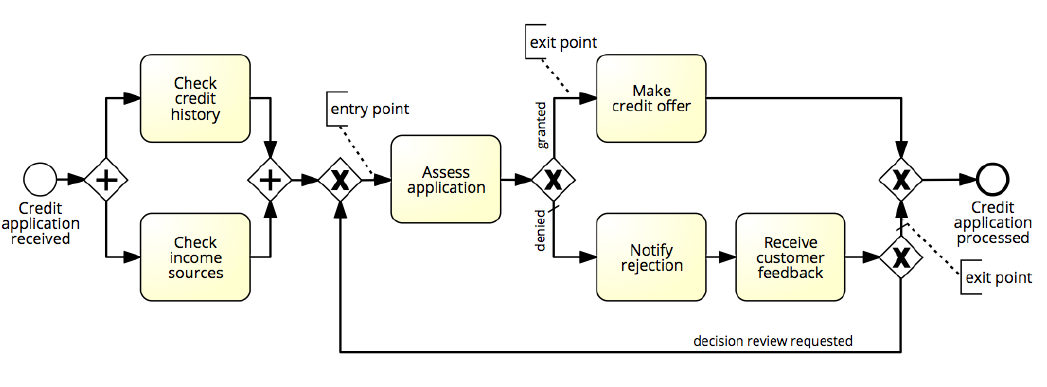
\includegraphics[width=0.75\linewidth]{capitolo 10/1.png}
\end{figure}
This involves defining a simulation scenario, which includes several key components:

Processing times of activities can be fixed values or follow a probability distribution. The choice of distribution depends on the nature of the activity. For example, a fixed value can be used for tasks with little variation in processing time, such as those performed by software applications. A normal distribution is suitable for simple and repetitive activities with minimal human judgment, like checking the completeness of an application. An exponential distribution is appropriate for complex activities involving analysis or decisions, such as assessing an application.
\begin{figure}[h!]
    \centering
    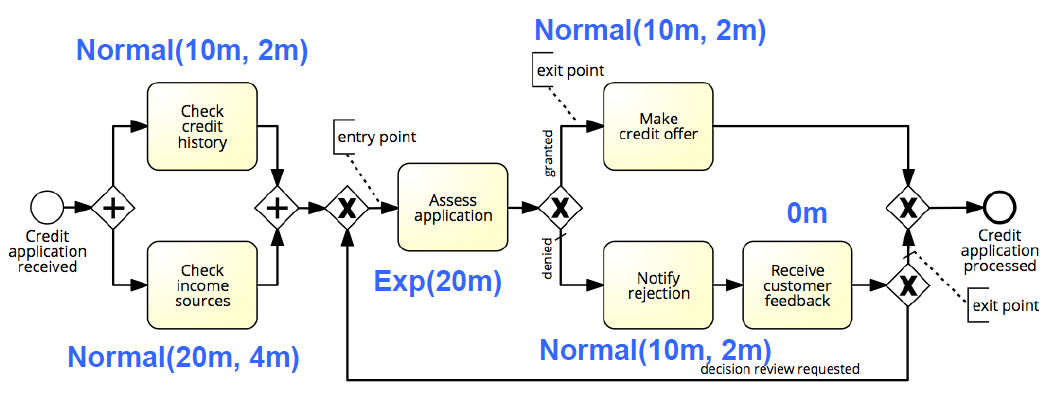
\includegraphics[width=0.75\linewidth]{capitolo 10/2.png}
\end{figure}
\begin{figure}[h!]
    \centering
    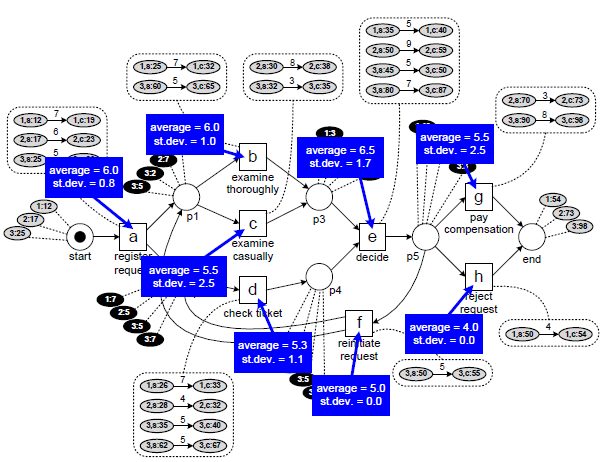
\includegraphics[width=0.75\linewidth]{capitolo 10/3.png}
\end{figure}

Branching probabilities are obtained by replaying the event-log traces onto the model. If the traces are not replayable, it may be necessary to create alignments.
\begin{figure}[h!]
    \centering
    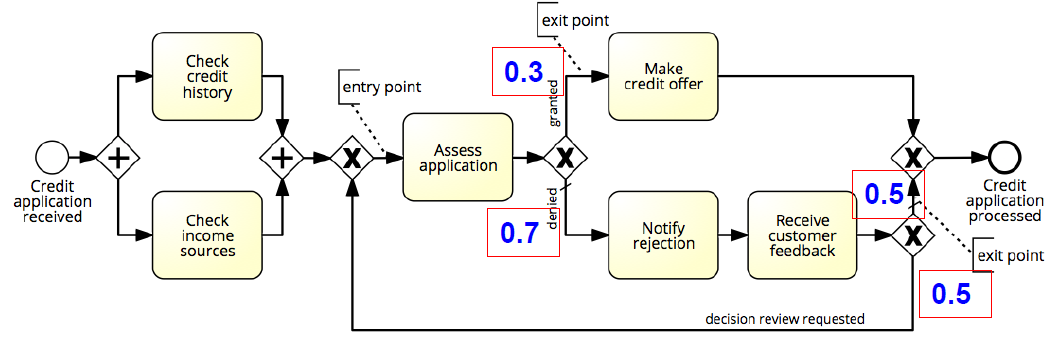
\includegraphics[width=0.75\linewidth]{capitolo 10/4.png}
\end{figure}
The arrival rate of process instances typically follows an exponential distribution with a given mean inter-arrival time. The arrival calendar, such as Monday to Friday from 9 am to 5 pm, or 24/7, should also be defined.

Resource pools should be defined with their name, size, cost per time unit, and availability (working calendar). In some tools, it is possible to define cost and calendar per resource rather than for the entire resource pool. A resource pool is a set of resources or roles that can perform a given activity. These pools can be constructed from event logs using algorithms to discover roles.
\begin{figure}[h!]
    \centering
    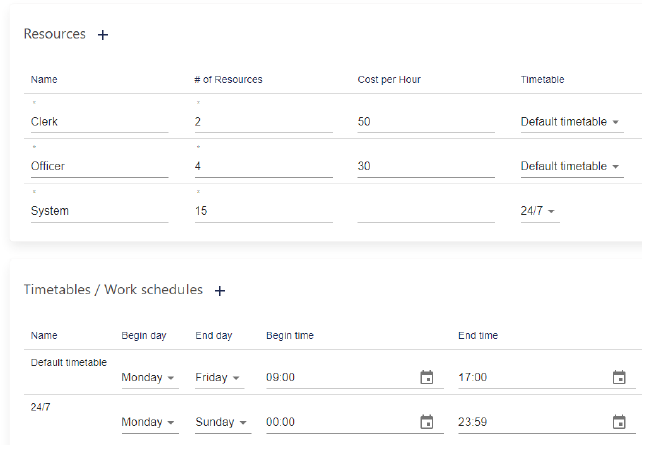
\includegraphics[width=0.75\linewidth]{capitolo 10/5.png}
\end{figure}
\begin{figure}[h!]
    \centering
    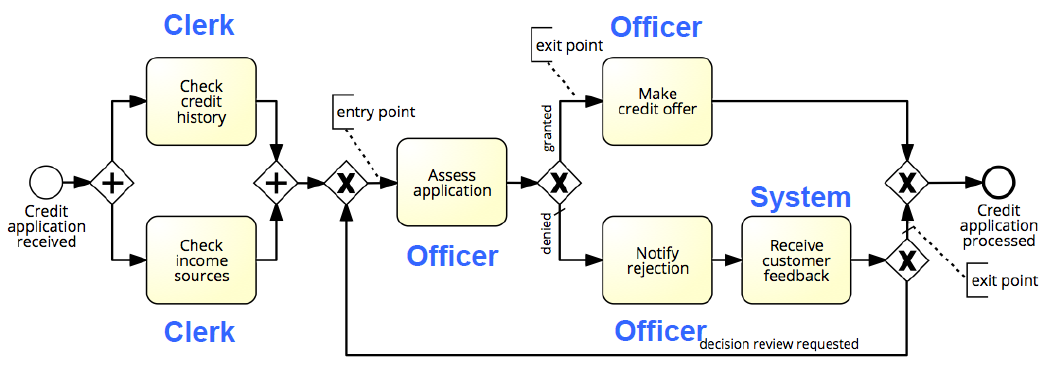
\includegraphics[width=0.75\linewidth]{capitolo 10/6.png}
\end{figure}

\subsection{Run the Simulation and Analyze Outputs}

After defining the simulation scenario, the next step is to run the simulation and analyze the outputs. This involves gathering performance data such as cost, time, and resource usage, and then calculating statistics from the collected data. It is important to analyze the simulation outputs carefully, as they provide insights into the behavior of the process under different scenarios.
\begin{figure}[h!]
    \centering
    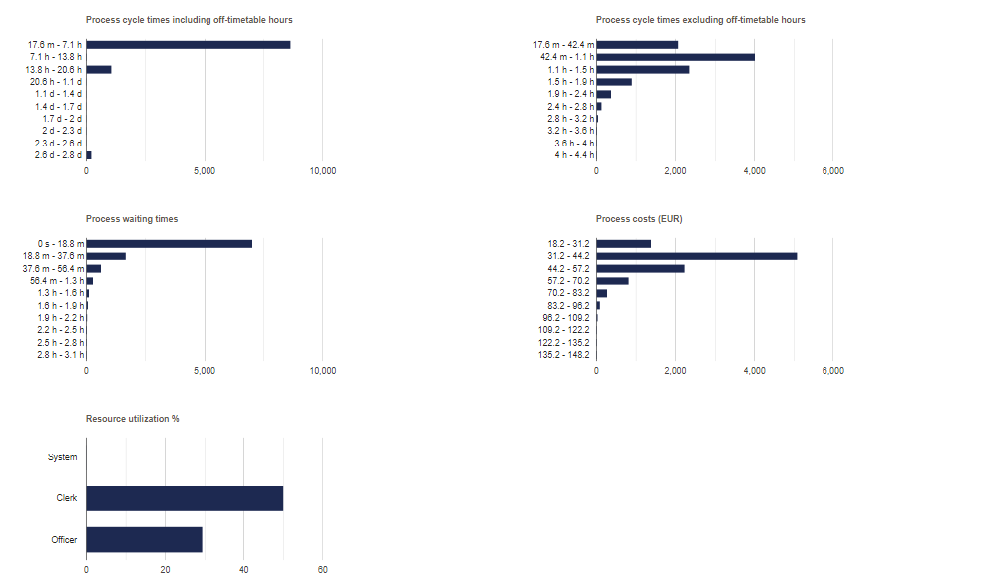
\includegraphics[width=1\linewidth]{capitolo 10/7.png}
\end{figure}

\begin{figure}[h!]
    \centering
    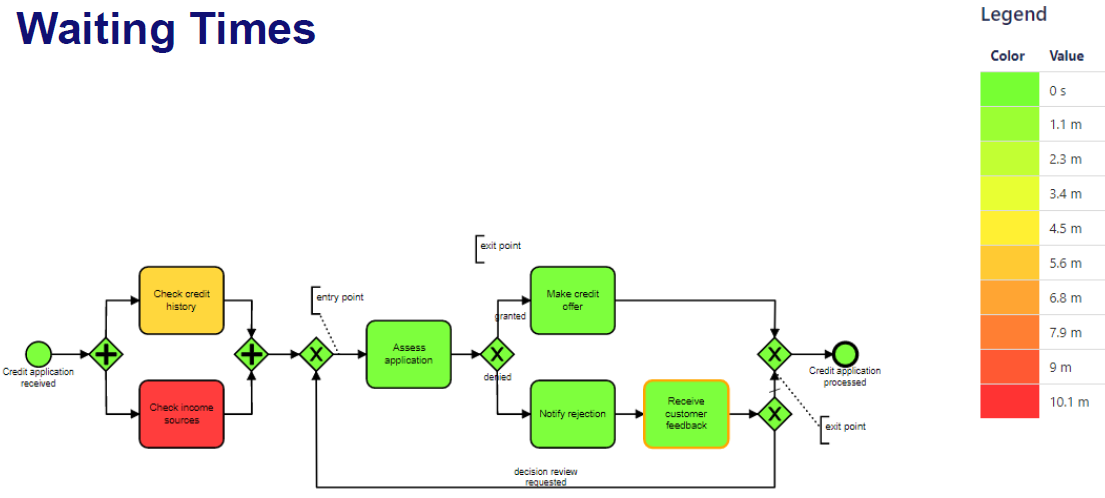
\includegraphics[width=0.75\linewidth]{capitolo 10/8.png}
\end{figure}

\newpage
\subsection{Repeat for Alternative Scenarios}

What-if analysis is a data-intensive simulation that involves inspecting the behavior of a complex system, such as a business process, under given hypotheses called scenarios. The goal is to measure how changes in a set of independent simulation variables impact dependent variables. Formulating a scenario enables building a hypothetical world that analysts can inspect and navigate for improvement.

\section{Pitfalls of Simulation}

While simulation is a powerful tool, it is not without its pitfalls. Stochasticity, data quality, and simplifying assumptions can all affect the reliability of simulation results.

\subsection{Stochasticity}

A single run does not provide information about the reliability of results. Therefore, multiple runs are necessary. If the runs are assumed to be mutually independent, one can calculate a confidence interval. For example, the cycle time is with 95\% confidence within the interval of [5,6] days. It is important to estimate the reliability of the estimates. The size of the confidence interval depends on the confidence level, the length, and the number of simulation runs.

\subsection{Warm-up and Cool-down Periods}

At the beginning of simulations, resources are 100\% free and queues at activities are empty, making the waiting and cycle times of the first traces not trustworthy. Therefore, simulation statistics should not be collected for the first X\% of the traces. Similarly, towards the end of simulations, when every trace of simulation is started, the activity queues become emptier and emptier, making the waiting and cycle times of the last traces not trustworthy. Therefore, simulation statistics should not be collected for the last Y\% of the traces.
\begin{figure}[h!]
    \centering
    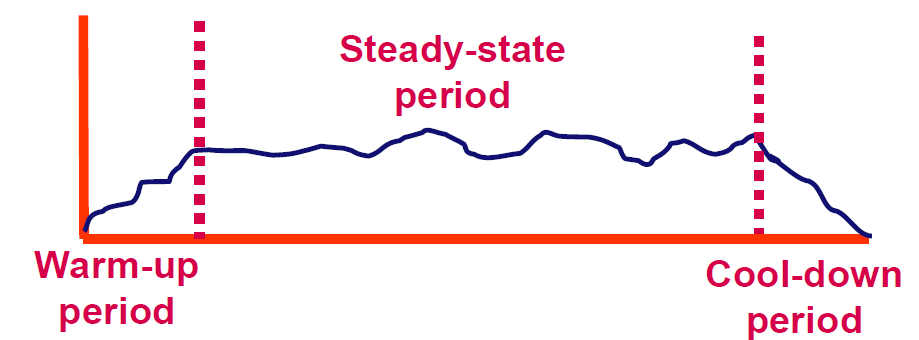
\includegraphics[width=0.75\linewidth]{capitolo 10/9.png}
\end{figure}
\subsection{Data Quality and Simplifying Assumptions}

Simulation results are only as trustworthy as the input data. Therefore, it is important to rely as little as possible on guesstimates and use actual observations where possible. Derive simulation scenario parameters from actual observations, such as applying process mining, and use statistical tools to check the fit of probability distributions. Simulate the as-is scenario and cross-check results against actual observations.

The closed-world assumption is typically used, limiting the input data to every aspect considered. In business process simulation, this means every event is stored in the system. However, some activities and happenings outside the system may not be stored, such as private phone calls, coffee breaks, or colleagues asking questions. To address this, model some invisible waiting-time activities and set their duration according to the waiting times.


    


\end{document}